%%%% Шаблон ВКР <<SPbPU-student-thesis-template>>  %%%%
%%
%%   Создан на основе глубокой переработки шаблона российских кандидатских и докторских диссертаций [1]. 
%%   
%%   Полный список различий может быть получен командами git.
%%   Лист авторов-составителей расположен в README.md файле.
%%   Подробные инструкции по использованию в [1,2].
%%   
%%   Рекомендуем установить TeX Live + TeXstudio
%%   <<Стандартная>> компиляция 2-3 РАЗА с помощью pdflatex + biber (для библиографии)     
%%  
%%%% Student thesis template <<SPbPU-student-thesis-template>> %%%%
%%
%%   Created on the basis of deepl modifification of the Russian candidate and doctorate thesis template [1]. 
%%   
%%   Full list of differences can be achieved by git commands.
%%   List of template authors can be seen in the README.md file.
%%   Detailed instructions of usage, see, please in [1,2].
%%     
%%   [1] github.com/AndreyAkinshin/Russian-Phd-LaTeX-Dissertation-Template 
%%   [2] Author_guide_SPBPU-student-thesis-template.pdf
%%   
%%   It is recommended to install TeX Live + TeXstudio   
%%   Default compilation 2-3 TIMES with pdflatex + biber (for the bibliography)
%%  
\input{template_settings/ch_preamble} % лучше не редактировать / please, keep unmodified

\setcounter{docType}{1} % лучше не редактировать / please, keep unmodified

%%%% Настройки автора / Author settings
%% 
%%%% Настройки автора 
%% 
%% 	 Пожалуйста, ознакомьтесь с функционалом шаблона из [1,2], а также с пакетами, подключенными в ch_preamble.
%% 
%%   Новым командам лучше присваивать уникальные имена.
%% 
%%%% Author settings
%% 
%%   Please, see all possible packages using the search in files of ch_preamble. 
%%   
%%   Please, for user-defined commands write only unique command titles.
%%
\usepackage{listings}

%%%% Подключение библиографии / Upload bibliography
%% 
%% 
\addbibresource{my_folder/my_biblio.bib} % 



%%%% Полезные настройки / Usefull settings
%% 
%% Раскомментируйте, чтобы
%%
%% pdf при открытии выравнивался по окну
%% pdf fit screen window
\hypersetup{
pdfstartview={FitBH}
}
%% перенумеровать все строки pdf
%% enumerate all lines in pdf 
%\usepackage{lineno}
%\linenumbers
%%
%% установить дату после названия ВКР - расскоментируйте код в title.tex
%% set data after the thesis title - uncomment code in title.tex
\let\ordinal\relax %avoid extra warning
\usepackage{datetime}



%% In case of deleting the following info, please, delete the examples in the chapter body.

%% В случае комментирования (удаления) следующего кода могут появиться ошибки при компиляции примеров, т.е. необходимо будет удалить и примеры в теле главы.

\newcommand{\overbar}[1]{\mkern 1.5mu\overline{\mkern-1.5mu#1\mkern-1.5mu}\mkern 1.5mu}

%http://tex.stackexchange.com/questions/16645/blackboard-italic-font
% for itallic sign of context K to be a parametr
\DeclareMathAlphabet{\mathbbmsl}{U}{bbm}{m}{sl}
\newcommand{\cont}[1][K]{\ensuremath{\mathbbmsl{#1}}}

%%ARROWS

%mu = math unit = 1em
%\mkern-18mu
%"minus quad"

%https://tex.stackexchange.com/a/389805/44348
\newcommand{\fcaarrow}[1]{%
	{}^{\scriptscriptstyle\bm{#1}}
}
%%%%%%%%%%%%%%%%%%%%%%% ARROWS from Formal Concept Analysis
% small and bold \uparrow
\newcommand{\uA}{\fcaarrow{{\uparrow\mkern-12mu}}}
% small and bold \downarrow
\newcommand{\dA}{\fcaarrow{\downarrow\mkern-2mu}}
% small and bold \uparrow+\downarrow
\newcommand{\ud}{\fcaarrow{\uparrow\mkern-12mu}\fcaarrow{\downarrow\mkern-2mu}}
% small and bold \downarrow+\uparrow
\newcommand{\du}{\fcaarrow{\downarrow\mkern-2mu}\fcaarrow{\uparrow\mkern-12mu}}


%http://tex.stackexchange.com/questions/74125/how-do-i-put-text-over-symbols
\newcommand\eqdef{\mathrel{\overset{\makebox[0pt]{\mbox{\normalfont\tiny def}}}{=}}} %\sffamily



%%% Правила задания нового окружения

\theoremstyle{myplain} % первая команда для ввода доказательств
\newtheorem{m-new-env-first}{Название\_окружения}[chapter] 
% вместо m-new-env-first необходимо подставить название нового окружения;
% вместо Название\_окружения необходимо подставить название окружения, выводящееся в pdf;
% последний параметр обеспечивает нумерацию в пределах главы не меняется


\theoremstyle{mydefinition} % первая команда для ввода окружений, не связанных с доказательствами
\newtheorem{m-new-env-second}{Название\_окружения}[chapter] 
% вместо m-new-env-second необходимо подставить название нового окружения;
% вместо Название\_окружения необходимо подставить название окружения, выводящееся в pdf;
% последний параметр обеспечивает нумерацию в пределах главы не меняется % добавляем свои команды / update your commands

\begin{document} % начало документа


%%% Внесите свои данные - Input your data
%%
%%
\newcommand{\Author}{А.Д.\,Кухто} % И.О. Фамилия автора 
\newcommand{\AuthorFull}{Кухто Андрей Денисович} % Фамилия Имя Отчество автора
\newcommand{\AuthorFullDat}{Кухто Андрею Денисовичу} % Фамилия Имя Отчество автора в дательном падеже (Кому? Студенту...)
\newcommand{\AuthorFullVin}{Кухто Андрея Денисовича} % в винительном падеже (Кого? что?  Програмиста ...)
\newcommand{\AuthorPhone}{+7-9XX-XXX-XX-XX} % номер телефорна автора для оперативной связи  
\newcommand{\Supervisor}{В.А.\,Пархоменко} % И. О. Фамилия научного руководителя
\newcommand{\SupervisorFull}{Пархоменко Владимир Андреевич} % Фамилия Имя Отчество научного руководителя
\newcommand{\SupervisorVin}{И.О.\,Фамилию} % И. О. Фамилия научного руководителя  в винительном падеже (Кого? что? Руководителя ...)
\newcommand{\SupervisorJob}{ст. преподователь ВШ ПИ} %
%\newcommand{\SupervisorJobVin}{должность} % в винительном падеже (Кого? что?  Програмиста ...)
%\newcommand{\SupervisorDegree}{к. т. н.} %
\newcommand{\SupervisorTitle}{звание} % 
%%
%%
%Руководитель, утверждающий задание
\newcommand{\Head}{А.В.\,Щукин} % И. О. Фамилия руководителя подразделения (руководителя ОП)
\newcommand{\HeadDegree}{Руководитель ОП}% Только должность:   
%Руководитель %ОП 
%Заведующий % кафедрой
%Директор % Высшей школы
%Зам. директора
\newcommand{\HeadDep}{} % заменить на краткую аббревиатуру подразделения или оставить пустым, если утверждает руководитель ОП

%%% Руководитель, принимающий заявление
\newcommand{\HeadAp}{И.О.\,Фамилия} % И. О. Фамилия руководителя подразделения (руководителя ОП)
\newcommand{\HeadApDegree}{Должность руководителя}% Только должность:   
%Руководитель ОП 
%Заведующий кафедрой
%Директор Высшей школы
\newcommand{\HeadApDep}{O} % заменить на краткую аббревиатуру подразделения или оставить пустым, если утверждает руководитель ОП
%%% Консультант по нормоконтролю
\newcommand{\ConsultantNorm}{В.А.\,Пархоменко} % И. О. Фамилия консультанта по нормоконтролю. ТОЛЬКО из числа ППС!
\newcommand{\ConsultantNormDegree}{ст. преподователь ВШ ПИ} %   
%%% Первый консультант
\newcommand{\ConsultantExtraFull}{Пархоменко Владимир Андреевич} % Фамилия Имя Отчетство дополнительного консультанта 
\newcommand{\ConsultantExtra}{В.А.\,Пархоменко} % И. О. Фамилия дополнительного консультанта 
\newcommand{\ConsultantExtraDegree}{ст. преподователь ВШ ПИ} % 
\newcommand{\ConsultantExtraVin}{И.О.\,Фамилию} % И. О. Фамилия дополнительного консультанта в винительном падеже (Кого? что? Руководителя ...)
\newcommand{\ConsultantExtraDegreeVin}{должность, степень} %  в винительном падеже (Кого? что? Руководителя ...)
%%% Второй консультант
\newcommand{\ConsultantExtraTwoFull}{Фамилия Имя Отчетство} % Фамилия Имя Отчетство дополнительного консультанта 
\newcommand{\ConsultantExtraTwo}{И.О.\,Фамилия} % И. О. Фамилия дополнительного консультанта 
\newcommand{\ConsultantExtraTwoDegree}{должность, степень} % 
\newcommand{\ConsultantExtraTwoVin}{И.О.\,Фамилию} % И. О. Фамилия дополнительного консультанта в винительном падеже (Кого? что? Руководителя ...)
\newcommand{\ConsultantExtraTwoDegreeVin}{должность, степень} %  в винительном падеже (Кого? что? Руководителя ...)
\newcommand{\Reviewer}{И.О.\,Фамилия} % И. О. Фамилия резензента. Обязателен только для магистров.
\newcommand{\ReviewerDegree}{должность, степень} % 
%%
%%
\renewcommand{\thesisTitle}{Разработка плагина Jenkins для визуализации статистики работы сборок Jenkins}
\newcommand{\thesisDegree}{работа бакалавра}% дипломный проект, дипломная работа, магистерская диссертация %c 2020
\newcommand{\thesisTitleEn}{Title of the thesis} %2020
\newcommand{\thesisDeadline}{09.01.2024}
\newcommand{\thesisStartDate}{02.10.2023}
\newcommand{\thesisYear}{2023}
%%
%%
\newcommand{\group}{з5130903/90301} % заменить вместо N номер группы
\newcommand{\thesisSpecialtyCode}{09.03.03}% код направления подготовки
\newcommand{\thesisSpecialtyTitle}{Прикладная информатика} % наименование направления/специальности
\newcommand{\thesisOPPostfix}{03} % последние цифры кода образовательной программы (после <<_>>)
\newcommand{\thesisOPTitle}{Интеллектуальные инфокоммуникационные технологии}% наименование образовательной программы
%%
%%
\newcommand{\institute}{
Институт компьютерных наук и кибербезопасности
%Институт компьютерных наук и~технологий
%Гуманитарный институт
%Инженерно-строительный институт
%Институт биомедицинских систем и технологий
%Институт металлургии, машиностроения и транспорта
%Институт передовых производственных технологий
%Институт прикладной математики и механики
%Институт физики, нанотехнологий и телекоммуникаций
%Институт физической культуры, спорта и туризма
%Институт энергетики и транспортных систем
%Институт промышленного менеджмента, экономики и торговли
}%
%%
%%




%%% Задание ключевых слов и аннотации
%%
%%
%% Ключевых слов от 3 до 5 слов или словосочетаний в именительном падеже именительном падеже множественного числа (или в единственном числе, если нет другой формы) по правилам русского языка!!!
%%
%%
\newcommand{\keywordsRu}{Визуализация, статистика, Jenkins, плагин, сборка, метрики сборки} % ВВЕДИТЕ ключевые слова по-русски
%%
%%
\newcommand{\keywordsEn}{Visualization, statistics, Jenkins, plugin, build, build metrics} % ВВЕДИТЕ ключевые слова по-английски
%%
%%
%% Реферат ОТ 1000 ДО 1500 знаков на русский или английский текст
%%
%Реферат должен содержать:
%- предмет, тему, цель ВКР;
%- метод или методологию проведения ВКР:
%- результаты ВКР:
%- область применения результатов ВКР;
%- выводы.

\newcommand{\abstractRu}{Целью работы является разработка плагина Jenkins для визуализации статистики работы сборок в инструментах совместного использования. Объект исследования — инструменты для сборки приложений. Предмет исследования — визуализация статистики работы сборок. Основными методами проведения работы являются методы сравнительного анализа аналогичных решений и методы объектно-ориентированного программирования. В результате работы разработан прототип плагина для визуализации статистики работы сборок Jenkins. Для визуализации и обработки метрик сборок применялись статистические показатели, разные типы диаграмм, а также анализ данных для прогнозирования значения метрик. Проведена апробация и тестирование разработки на реальном проекте с открытым исходным кодом в системе Jenkins. Область применения разработанного плагина - промышленная разработка программных продуктов, которые собираются и тестируются с использованием CI инструмента Jenkins.
} % ВВЕДИТЕ текст аннотации по-русски
%%
%%
\newcommand{\abstractEn}{The purpose of the work is to develop a Jenkins plugin for visualizing build statistics in sharing tools. The object of study is tools for building applications. The subject of the study is visualization of assembly operation statistics. The main methods of carrying out the work are methods of comparative analysis of similar solutions and methods of object-oriented programming. As a result of the work, a prototype plugin was developed for visualizing statistics on the operation of Jenkins builds. To visualize and process assembly metrics, statistical measures, different types of charts, and data analysis were used to predict the value of metrics. Approbation and testing of the development was carried out on a real open source project in the Jenkins system. The scope of application of the developed plugin is industrial development of software products that are assembled and tested using the Jenkins CI tool.} % ВВЕДИТЕ текст аннотации по-английски


%%% РАЗДЕЛ ДЛЯ ОФОРМЛЕНИЯ ПРАКТИКИ
%Место прохождения практики
\newcommand{\PracticeType}{Отчет о прохождении % 
	%стационарной производственной (технологической (проектно-технологической)) %
	преддипломной % тип и вид ЗАМЕНИТЬ
	практики}

\newcommand{\Workplace}{СПбПУ, ИКНК, ВШПИ г. Санкт-Петербург, ул. Обручевых, д. 1, лит. В} % TODO Rename this variable

% Даты начала/окончания
\newcommand{\PracticeStartDate}{%
19.12.2023%
%	22.06.2020
}%
\newcommand{\PracticeEndDate}{%
	09.01.2024%
%	18.07.2020%
}%
%%

\newcommand{\School}{
	Название высшей школы
%	Высшая школа интеллектуальных систем и~суперкомпьютерных~технологий 
}
\newcommand{\practiceTitle}{Разработка плагина Jenkins для визуализации статистики работы сборок Jenkins}


%% ВНИМАНИЕ! Необходимо либо заменить текст аннотации (ключевых слов) на русском и английском, либо удалить там весь текст, иначе в свойства pdf-отчета по практике пойдет шаблонный текст.

%%% Не меняем дальнейшую часть - Do not modify the rest part
%%
%%
%%
%%
\ifnumequal{\value{docType}}{1}{% Если ВКР, то...
	\newcommand{\DocType}{Выпускная квалификационная работа}
	\newcommand{\pdfDocType}{\DocType~(\thesisDegree)} %задаём метаданные pdf файла
	\newcommand{\pdfTitle}{\thesisTitle}
}{% Иначе 
	\newcommand{\DocType}{\PracticeType}
	\newcommand{\pdfDocType}{\DocType} %задаём метаданные pdf файла
	\newcommand{\pdfTitle}{\practiceTitle}
}%
\newcommand{\HeadTitle}{\HeadDegree~\HeadDep}
\newcommand{\HeadApTitle}{\HeadApDegree~\HeadApDep}
\newcommand{\thesisOPCode}{\thesisSpecialtyCode\_\thesisOPPostfix}% код образовательной программы
\newcommand{\thesisSpecialtyCodeAndTitle}{\thesisSpecialtyCode~\thesisSpecialtyTitle}% Код и наименование направления/специальности
\newcommand{\thesisOPCodeAndTitle}{\thesisOPCode~\thesisOPTitle} % код и наименование образовательной программы
%%
%%
\hypersetup{%часть болка hypesetup в style
		pdftitle={\pdfTitle},    % Заголовок pdf-файла
		pdfauthor={\AuthorFull},    % Автор
		pdfsubject={\pdfDocType. Шифр и наименование направления подготовки: \thesisSpecialtyCodeAndTitle. \abstractRu},      % Тема
		pdfcreator={LaTeX, SPbPU-student-thesis-template},     % Приложение-создатель
%		pdfproducer={},  % Производитель, Производитель PDF % будет выставлена автоматически
		pdfkeywords={\keywordsRu}
}
%%
%%
%% вспомогательные команды
\newcommand{\firef}[1]{рис.\ref{#1}} %figure reference
\newcommand{\taref}[1]{табл.\ref{#1}}	%table reference
%%
%%
%% Архивный вариант задания ключевых слов, аннотации и благодарностей 
% Too hard to export data from the environment to pdf-info
% https://tex.stackexchange.com/questions/184503/collecting-contents-of-environment-and-store-them-for-later-retrieval
%заменить NewEnviron на newenvironment для распознавания команды в TexStudio
%\NewEnviron{keywordsRu}{\noindent\MakeUppercase{\BODY}}
%\NewEnviron{keywordsEn}{\noindent\MakeUppercase{\BODY}}
%\newenvironment{abstractRu}{}{}
%\newenvironment{abstractEn}{}{}
%\newenvironment{acknowledgementsRu}{\par{\normalfont \acknowledgements.}}{}
%\newenvironment{acknowledgementsEn}{\par{\normalfont \acknowledgementsENG.}}{}


%%% Переопределение именований %%% Не меняем - Do not modify
%\newcommand{\Ministry}{Минобрнауки России} 
\newcommand{\Ministry}{Министерство науки и высшего образования Российской~Федерации} %с 2020
\newcommand{\SPbPU}{Санкт-Петербургский политехнический университет Петра~Великого}
\newcommand{\SPbPUOfficialPrefix}{Федеральное государственное автономное образовательное учреждение высшего образования}
\newcommand{\SPbPUOfficialShort}{ФГАОУ~ВО~<<СПбПУ>>}
%% Пробел между И. О. не допускается.
\renewcommand{\alsoname}{см. также}
\renewcommand{\seename}{см.}
\renewcommand{\headtoname}{вх.}
\renewcommand{\ccname}{исх.}
\renewcommand{\enclname}{вкл.}
\renewcommand{\pagename}{Pages}
\renewcommand{\partname}{Часть}
\renewcommand{\abstractname}{\textbf{Аннотация}}
\newcommand{\abstractnameENG}{\textbf{Annotation}}
\newcommand{\keywords}{\textbf{Ключевые слова}}
\newcommand{\keywordsENG}{\textbf{Keywords}}
\newcommand{\acknowledgements}{\textbf{Благодарности}}
\newcommand{\acknowledgementsENG}{\textbf{Acknowledgements}}
\renewcommand{\contentsname}{Content} % 
%\renewcommand{\contentsname}{Содержание} % (ГОСТ Р 7.0.11-2011, 4)
%\renewcommand{\contentsname}{Оглавление} % (ГОСТ Р 7.0.11-2011, 4)
\renewcommand{\figurename}{Рис.} % Стиль СПбПУ
%\renewcommand{\figurename}{Рисунок} % (ГОСТ Р 7.0.11-2011, 5.3.9)
\renewcommand{\tablename}{Таблица} % (ГОСТ Р 7.0.11-2011, 5.3.10)
%\renewcommand{\indexname}{Предметный указатель}
\renewcommand{\listfigurename}{Список рисунков}
\renewcommand{\listtablename}{Список таблиц}
\renewcommand{\refname}{\fullbibtitle}
\renewcommand{\bibname}{\fullbibtitle}

\newcommand{\chapterEnTitle}{Сhapter title} % <- input the English title here (only once!) 
\newcommand{\chapterRuTitle}{Название главы}          % <- введите 
\newcommand{\sectionEnTitle}{Section title} %<- input subparagraph title in english
\newcommand{\sectionRuTitle}{Название подраздела} % <- введите название подраздела по-русски
\newcommand{\subsectionEnTitle}{Subsection title} % - input subsection title in english
\newcommand{\subsectionRuTitle}{Название параграфа} % <- введите название параграфа по-русски
\newcommand{\subsubsectionEnTitle}{Subsubsection title} % <- input subparagraph title in english
\newcommand{\subsubsectionRuTitle}{Название подпараграфа} % <- введите название подпараграфа по-русски % Заполнить сведения, 
										 % в т.ч. ключевые слова и аннотацию.

%%% Титульник ВКР / Thesis title 
%%
%% добавить лист в pdf-навигацию 
%% add to pdf navigation menu
%%
\pdfbookmark[-1]{\pdfTitle}{tit}
%%
\thispagestyle{empty}%
\makeatletter
\newgeometry{top=2cm,bottom=2cm,left=3cm,right=1cm,headsep=0cm,footskip=0cm}
\savegeometry{NoFoot}%
\makeatother


%%% Распечатать версию документа / Print document version
%%
\begin{flushright}
%	\vspace{0pt plus0.1fill}
	\boxed{\small
		\begin{tabular}{r} 
			\textbf{Пример ВКР <<SPbPU-student-thesis-template>>.} %\\ % перенос на новую строку
			\textbf{Версия от \today % \; время:  \currenttime. % время версии
			}
		\end{tabular}
	} %end boxed
%	\vspace*{-5pt} % раскомментировать, если не хватает места
	\vspace{0pt plus0.1fill} % раскоментировать, если хватает места
\end{flushright}

{\centering%
	\Ministry\\
	\SPbPU\\
	{%\bfseries %2020 - указание на изменения, которые могут быть введены в 2020 году
		\institute}
\par}%


\vspace{0pt plus1fill} %число перед fill = кратность относительно некоторого расстояния fill, кусками которого заполнены пустые места


\noindent
\begin{minipage}{\linewidth}
	\vspace{\mfloatsep} % интервал 
	\begin{tabularx}{\linewidth}{Xl}
	&Работа допущена к защите     \\
	&\HeadTitle     \\			
	&\underline{\hspace*{0.1\textheight}} \Head     \\
	&<<\underline{\hspace*{0.05\textheight}}>> \underline{\hspace*{0.1\textheight}} \thesisYear~г.  \\ 
	\end{tabularx}
	\vspace{\mfloatsep} % интервал 	
\end{minipage}


\vspace{0pt plus2fill} %


{\centering%
	
	\MakeUppercase{\bfseries{}\DocType} \\ 
	\MakeUppercase{\thesisDegree}%


%\intervalS% %ОБЯЗАТЕЛЬНО ДОБАВИТЬ ОТСТУП, ЕСЛИ ХВАТАЕТ МЕСТА
{\centering%
	\MakeUppercase{\bfseries{\thesisTitle}}}%

}\par%

%\intervalS% %ОБЯЗАТЕЛЬНО ДОБАВИТЬ ОТСТУП, ЕСЛИ ХВАТАЕТ МЕСТА
%по специальности % для специалистов
\noindent	по направлению подготовки \thesisSpecialtyCodeAndTitle{}\\% для бакалавров и магистров 
%\noindent Направленность  % для специалистов
\noindent	Направленность (профиль)	\thesisOPCodeAndTitle % для бакалавров и магистров
% Лучше по~профилю, но что делать, так составили Положение
\par%





\vspace{4mm plus2fill}%

\noindent
\begin{tabularx}{\linewidth}{lXl}
	Выполнил              &	   &             \\
	студент гр.~\group     &    & \Author     \\[\mfloatsep]

	Руководитель 		  &    &             \\
	\SupervisorJob,		  &    &             \\
	\SupervisorTitle 	  &    & \Supervisor \\[\mfloatsep]
	
	Консультант  &    &  \\   	
	по нормоконтролю 		 	  &    & \ConsultantNorm  % обязателен
\end{tabularx} %


%
\vspace{0pt plus4fill}% 


\begin{center}%
Санкт-Петербург\\
\thesisYear
\end{center}%
\restoregeometry
\newpage					 % Титульный лист
										 % Убираем footnotes, консультанта, если нет

%%%% Начало оформления заголовка - оставить без изменений !!! %%%%
\input{my_folder/task_settings}	% настройки - начало 
	
				{%\normalfont %2020
						\MakeUppercase{\SPbPU}}\\
				\institute

\par}\intervalS% завершает input

				\noindent
				\begin{minipage}{\linewidth}
				\vspace{\mfloatsep} % интервал 	
				\begin{tabularx}{\linewidth}{Xl}
					&УТВЕРЖДАЮ      \\
					&\HeadTitle     \\			
					&\underline{\hspace*{0.1\textheight}} \Head     \\
					&<<\underline{\hspace*{0.05\textheight}}>> \underline{\hspace*{0.1\textheight}}  \\  
				\end{tabularx}
				\vspace{\mfloatsep} % интервал 	
				\end{minipage}

\intervalS{\centering\bfseries%

				ЗАДАНИЕ\\
				на выполнение %с 2020 года 
				%по выполнению % до 2020 года
				выпускной квалификационной работы


\intervalS\normalfont%

				студенту \uline{\AuthorFullDat{} гр.~\group}


\par}\intervalS%
%%%%
%%%% Конец оформления заголовка  %%%%
 	
	
	
\begin{enumerate}[1.]
	\item Тема работы: {\expandafter \ulined \thesisTitle.}
	%\item Тема работы (на английском языке): \uline{\thesisTitleEn.} % вероятно после 2021 года
	\item Срок сдачи студентом законченной работы: \uline{\thesisDeadline.} 
	\item Исходные данные по работе: \uline{документация по Jenkins \cite{jenkins}, Java \cite{java}, TeamCity \cite{tc}.}%
	\printbibliographyTask % печать списка источников % КОММЕНТИРУЕМ ЕСЛИ НЕ ИСПОЛЬЗУЕТСЯ
	% В СЛУЧАЕ, ЕСЛИ НЕ ИСПОЛЬЗУЕТСЯ МОЖНО ТАКЖЕ ЗАЙТИ В setup.tex и закомментировать \vspace{-0.28\curtextsize}
	\item Содержание работы (перечень подлежащих разработке вопросов):
	\begin{enumerate}[label=\theenumi\arabic*.]
		\item Обзор инструментов сборок для совместной работы.
		\item Исследование плагинов визуализации статистики работы сборок Jenkins.
		\item Разработка плагина визуализации статистики работы сборок для системы Jenkins.
		\item Тестирование и апробация плагина в системе Jenkins. 
	\end{enumerate}
	\item Перечень графического материала (с указанием обязательных чертежей): 
	\begin{enumerate}[label=\theenumi\arabic*.]
		\item Use-case, Class и IDEF0 диаграммы.
		\item Архитектура разработанного плагина.
	\end{enumerate}	
		\item Консультанты по работе:
		\begin{enumerate}[label=\theenumi\arabic*.] 
		%\item  \uline{\emakefirstuc{\ConsultantExtraDegree}, \ConsultantExtra.} % закомментировать при необходимости, идёт первый по порядку.
		\item \uline{\emakefirstuc{\ConsultantNormDegree}, \ConsultantNorm{} (нормоконтроль).} %	Обязателен для всех студентов
	\end{enumerate}
		\item Дата выдачи задания: \uline{\thesisStartDate.}
\end{enumerate}

\intervalS%можно удалить пробел

Руководитель ВКР \uline{\hspace*{0.1\textheight} \Supervisor}


%\intervalS%можно удалить пробел

%Консультант\footnote{В случае, если есть консультант, отличный от консультанта по нормоконтролю.}  \uline{\hspace*{0.1\textheight}\ConsultantExtra}


\intervalS%можно удалить пробел

%Консультант по нормоконтролю \uline{\hspace*{0.1\textheight} \ConsultantNorm}%ПОКА НЕ ТРЕБУЕТСЯ, Т.К. ОН У ВСЕХ ПО УМОЛЧАНИЮ

Задание принял к исполнению \uline{\thesisStartDate}

\intervalS%можно удалить пробел

Студент \uline{\hspace*{0.1\textheight}  \Author}



\input{my_folder/task_settings_restore}	% настройки - конец					 % Задание 
										 % Для сдачи в высшую школу компилируем двухсторонний My_task.tex 
										 % После подписания задания изменение его содержания и оформления запрещено

%% Не менять - Do not modify
%%\input{my_folder/summary_settings} 
\chapter*[Count-me]{Реферат} % * - не нумеруем
\thispagestyle{empty}% удаляем параметры страницы
%\setcounter{sumPageFirst}{\value{page}}
%sumPageFirst \arabic{sumPageFirst}
%
%
%% Возможность проверить другие значения счетчиков - debugging
%\ref*{TotPages}~с.,
%\formbytotal{mytotalfigures}{рисун}{ок}{ка}{ков},
%\formbytotal{mytotaltables}{таблиц}{у}{ы}{},
%There are \TotalValue{mytotalfigures} figures in this document
%There are \TotalValue{mytotalfiguresInApp} figuresINAPP in this document
%There are \TotalValue{mytotaltables} tables in this document
%There are \TotalValue{mytotaltablesInApp} figuresINAPP in this document
%There are \TotalValue{myappendices} appendix chapters in this document
%\total{citenum}~библ. наименований.



%% Для того, чтобы значения счетчиков корректно отобразились, необходимо скомпилировать файл 2-3 раза
На \total{mypages}~c.,  
\formbytotal{myfigures}{рисун}{ок}{ка}{ков},
\formbytotal{mytables}{таблиц}{у}{ы}{},
\formbytotal{myappendices}{приложен}{ие}{ия}{ий}%.  

%\noindent
{\MakeUppercase{Ключевые слова: \keywordsRu}.}% Ключевые слова из renames.tex

Тема выпускной квалификационной работы: <<\thesisTitle>>.


\abstractRu % Аннотация из renames.tex

 % УДАЛИТЬ. Повтор иллюстрации переноса текста на вторую страницу



\printTheAbstract % не удалять


\total{mypages}~pages, 
\total{myfigures}~figures, 
\total{mytables}~tables,
\total{myappendices}~appendices%.

%\noindent
{\MakeUppercase{Keywords: \keywordsEn}.} % Ключевые слова из renames.tex 
	
The subject of the graduate qualification work is <<\thesisTitleEn>>.
	
	
\abstractEn % Аннотация из renames.tex

	


%% Не менять - Do not modify
\thispagestyle{empty}
%\setcounter{sumPageLast}{\value{page}} %сохранили номер последней страницы Задания
%\setcounter{sumPages}{\value{sumPageLast}-\value{sumPageFirst}}
%sumPageLast \arabic{sumPageLast}
%
%sumPages \arabic{sumPages}
%\restoregeometry % восстанавливаем настройки страницы
%\input{my_folder/summary_settings_restore}	% настройки - конец			 	 % Реферат 
										 % Убираем footnotes, дубли команд \abstractEn и \abstractRu 
										

\input{my_folder/contents}  	         % Оглавление


\chapter*{Введение} % * не проставляет номер
\addcontentsline{toc}{chapter}{Введение} % вносим в содержание

Сегодня разработка информационных систем достаточно сложный процесс, который состоит, как правило, из следующих основных этапов: анализ требований заказчика, проектирование системы, разработка, тестирование и доставка приложения потенциальному заказчику. 

Для упрощения процесса разработки программного обеспечения в настоящий момент широко применяются практики DevOps, одной из которых является Continuous Integration, Continuous Delivery -- CI/CD - непрерывная интеграция, сборка и доставка ССЫЛКА???. Существует множество средств CI, которые применяются в промышленной разработке: TeamCity, Jenkins, Gitlab CI и другие.

Под \textit{сборкой программного продукта} будем подразумевать процесс объединения отдельных файлов и компонентов программы в единый исполняемый файл или пакет, который включает в себя компиляцию, связывание модулей, оптимизацию и другие операции, необходимые для создания готового к выполнению приложения \cite{build}.

Будем различать понятие сборки программного продукта и \textit{сборки} в инструментах CI/CD, таких как Jenkins, которые обычно используются \textit{командой для совместной работы над одним проектом}. \textit{Сборка Jenkins} — это набор задач, которые выполняются последовательно, как определено пользователем \cite{jenkinsjob}.

Одним из лучших средств CI, в котором доступно много функций ''из коробки'' является TeamCity компании Jetbrains. TeamCity - мощный и сложный инструмент, который использовался крупными ИТ компаниями в промышленной разработке до 2022 года. Одним из главных недостатков TeamCity является то, что это платное решение, лицензия обходится ИТ компания достаточно дорого, также недостатком является то, что компания Jetbrains покинула ИТ сектор РФ. Для того, чтобы преодолеть данные проблемы ИТ компании РФ начали поиск бесплатных средств с открытым исходным кодом. Одним из таких средств является Jenkins - средство CI, которое всегда пользовалось популярностью у разработчиков при локальной разработке решений с открытым исходным кодом. 

Jenkins обладает меньшим функционалом по сравнению с TeamCity, но имеет много подключаемых плагинов, которые могут помочь заменить или даже улучшить те функции, которые требуется разработчикам в процессе тестирования, сборки и доставки приложений.

\textbf{Актуальность исследования.} На данный момент в Jenkins нет плагина, который полностью заменяет модуль визуализации статистики (Build Configuration Statistics) из TeamCity???. Этот плагин/модуль требуется для того чтобы отслеживать состояние отдельных конфигураций сборки с течением времени, плагин собирает статистические данные по всей истории сборки и отображает их в виде наглядных диаграмм.

\textbf{Степень разработанности проблемы.} Среди имеющихся плагинов Jenkins есть те, которые реализует частичный функционал модуля из TeamCity, например, отображение графика продолжительности сборок за период. Подробнее о недостатках таких средств будет описано в сравнительном анализе и обзоре аналогов. 

%В данной работе будет разработан плагин, который обеспечит визуализацию статистики работы сборок.

\textbf{Объект исследования} — инструменты для сборки приложений в инструментах совместного использования.

\textbf{Предмет исследования} — визуализация статистики работы сборок.

\textbf{Цель} - разработать плагин Jenkins для визуализации статистики работы сборок в инструментах совместного использования.

Задачи:
 
\begin{enumerate}
	\item Изучить инструменты сборки приложений.
	
	\item Изучить особенности CI/CD, Jenkins, работу и характеристики сборок Jenkins.
	
	\item Описать метрики и статистики, которые могут собираться по результатам работы сборок Jenkins.
	
	\item Изучить методы разработки плагинов Jenkins.
	
	\item Провести проектирование плагина и описать архитектуру.
	
	\item Реализовать плагин.
	
	\item Провести тестирование и апробацию плагина. 
	
\end{enumerate}

Основными \textbf{методами} проведения работы являются методы сравнительного анализа аналогичных решений и методы объектно-ориентированного программирования.




%% Вспомогательные команды - Additional commands
%\newpage % принудительное начало с новой страницы, использовать только в конце раздела
%\clearpage % осуществляется пакетом <<placeins>> в пределах секций
%\newpage\leavevmode\thispagestyle{empty}\newpage % 100 % начало новой строки	    	 % Введение

%% Начало основной части
\chapter{Анализ средств сборки и визуализации программного обеспечения} \label{ch1}

% не рекомендуется использовать отдельную section <<введение>> после лета 2020 года
%\section{Введение. Сложносоставное название первого параграфа первой главы для~демонстрации переноса слов в содержании} \label{ch1:intro}

В первой главе рассмотрим:

\begin{enumerate}
	\item Процесс и инструменты сборки приложения.
	
	\item Обзор и сравнительный анализ средств CI/CD в контексте сборок приложения.
	
	\item Понятие статистик и визуализации сборок в контексте инструментов CI/CD.
	
	\item Обзор и сравнительный анализ плагинов Jenkins по визуализации статистики работы сборок.
	
	\item Требования к разработке.
	
	
\end{enumerate}

\section{Обзор и сравнительный анализ средств сборки программного обеспечения} \label{ch1:sec1}

Для осуществления сборки программного продукта существует множество инструментов, какое средство использовать определяют не только из преимуществ и недостатков этих средств, но и исходя из того, какой используется язык программирования, фреймворк и окружение.
На данный момент существует большое количество инструментов сборки приложения. 

Maven — инструмент для автоматизации сборки проектов, который используется с Java приложениями. Maven решает несколько проблем \cite{maven}:

\begin{itemize}
	\item  упрощение процесса сборки;
	\item обеспечение единой системы сборки;
	\item предоставление информации о проекте;
	\item упрощение работы с зависимостями, включая их автоматическое обновление.
\end{itemize}

Gradle — система автоматизации сборки, которая также часто используется для Java разработки. Gradle включает в себя следующие возможности \cite{gradle}:

\begin{itemize}
	\item декларативное описание сборки;
	\item управление зависимостями;
	\item создание многомодульных проектов;
	\item плагины.
\end{itemize}

Для проектов на JavaScript для управления зависимостями и сборками может использоваться npm в связке с Webpack. Webpack это инструмент для сборки и оптимизации приложений Node.js. Преимущества инструмента  \cite{webpack}:

\begin{itemize}
	\item разбивки пакетов на мелкие фрагменты;
	\item поддержка плагинов;
	\item большое сообщество.
\end{itemize}

Также данный сборщик обладает такими недостатками, как высокий порог вхождения и низкая скорость сборки.

Также необходимо отметить, что в отличии от компилируемых языков, таких как Java, приложения на интерпретируемом языке Python могут запускаться без сборки прямо из командной строки, а для управления зависимостями в Python используется инструмент pip.

Существуют также и другие инструменты сборки для приложений написанных на разных языках программирования. Все их удобно использовать при локальной разработке над небольшими проектами, но когда рассматривается вопрос о разработке большого продукта, в работе над которым задействуется целая команда разработчиков и тестировщиков, для уменьшения затрат на разработку, в первую очередь временных, следует внедрять DevOps практики и CI/CD подходы.

Инструменты CI/CD позволят взаимодействовать с репозиторием гита, проводить сборку продукта автоматически по заданному времени или по наличию новых коммитов, прогонять тесты после каждого изменения разработчика, производить установку на различные стенды, а также выполнять сборку различных компонентов системы одновременно и доставлять продукт заказчику. Перейдем к рассмотрению особенностей CI/CD инструментов, а затем рассмотрим сравнение их между собой.


\section{Особенности и сравнительный анализ CI/CD систем} \label{ch1:sec2}

CI/CD — это технология автоматизации тестирования и доставки/развертывания готового приложения заказчику  \cite{cicd}. Данная технология стала неотъемлемой составляющей DevOps методологии и помогает сократить временные  ресурсные затраты в процессе современного жизненного цикла приложения, когда до заказчика изначально доходит минимально жизнеспособный продукт (MVP), а затем дорабатывается с учетом новых требований заказчика, т.е. идет непрерывная разработка новых версий продукта.

Преимущества CI/CD подхода \cite{plusci}:

\begin{itemize}
	\item упрощение разработки - позволяет разработчикам распределять приоритеты и сконцентрироваться на самых важных аспектах;
	\item улучшение качества кода -  качество кода проверяется до того, как он достигнет среды тестирования, проблемы в коде могут быть выявлены на ранних стадиях;
	\item более короткие циклы тестирования - меньший объем кода для проверки, становиться проще определить проблемы в процессе развертывания;
	\item более простой мониторинг изменений - меньший объем кода для проверки;
	\item более легкий откат - меньшие усилия для отката приложения к предыдущей версии при возникновении проблем в новой версии.
\end{itemize}

Этапы разработки и принцип CI/CD подхода можно отразить с помощью рисунка 1.

\begin{figure}[ht!] 
	\center
	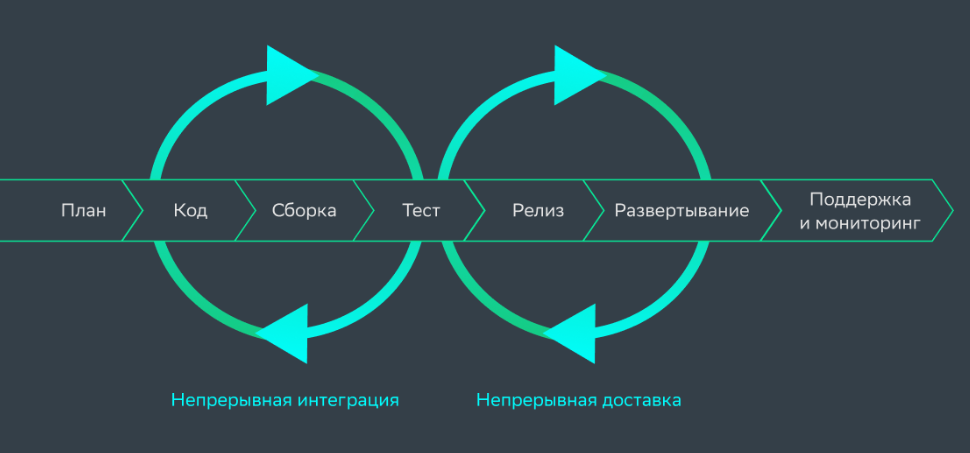
\includegraphics [scale=0.67] {my_folder/images//cicdalter}
	\caption{Цикл CI/CD \cite{cycleci}} 
	\label{fig:ci-cd}  
\end{figure}

\section{Обзор и сравнительный анализ средств CI/CD} \label{ch1:sec3}



На данный момент существует множеств инструментов CI/CD, которые обладают своими преимуществами и недостатками, были выделены самые распространенные системы:

\begin{itemize}
	\item TeamCity;
	\item Jenkins;
	\item GitLab CI;
	\item CircleCI;
	\item Bamboo.
\end{itemize}




Jenkins — это автономный сервер автоматизации с открытым исходным кодом, который можно использовать для автоматизации всех видов задач, связанных со сборкой, тестированием, доставкой или развертыванием программного обеспечения \cite{jenkins}.

TeamCity - это сервер CI от компании Jetbrains  \cite{tc}, который позволяет запускать параллельные сборки одновременно на разных платформах и средах, а также настраивать статистику по продолжительности сборки, уровню успешности, качеству кода и пользовательским метрикам.

GitLab CI - сервер CI от компании GitLab \cite{gitlab}, которая также предоставляет одноименный репозиторий Git. GitLab CI/CD может обнаруживать ошибки на ранних этапах цикла разработки и гарантировать, что весь код, развернутый в рабочей среде, соответствует установленным стандартам кода.

CircleCI - сервер CI \cite{circle}, который позволяет настроить для эффективной работы очень сложных конвейеров кэширование, кэширование уровня Docker и классы ресурсов для работы на более быстрых машинах.

Bamboo — это инструмент непрерывной интеграции и доставки  \cite{bamboo}, который связывает автоматизированные сборки, тесты и выпуски в единый рабочий процесс.

В таблице 1.1 указан, краткий сравнительный анализ плагинов. Стоит сразу отметить, что \textit{сравнение платных и бесплатных решений не корректно}, поскольку организации, которые выпускают коммерческие продукты обладают куда большими возможностями в сравнении с компаниями, которые не берут плату за использование своего продукта. Что наглядно видно из сравнительного анализа Jenkins с остальными средствами CI.

Особое внимание следует уделить критерию OpenSource, этот критерий является достаточно важным с учетом, того, что многие компании после 2022 года ушли из РФ, тем самым стали либо недоступны, либо прекратили лицензировании и стали менее безопасными, т.к. новые версии продуктов больше недоступны и проблемы с безопасностью и другими дефектами не будут исправлены/доступны на территории РФ. Также критерий важен тем, что даже при наличии действия продуктов компаний, они обходилось крупным ИТ-компаниям достаточно дорого.

\begin{table}
    \centering
    \caption{Сравнительный анализ инструментов CI/CD}
    \begin{tabular}{|p{3cm}|p{2cm}|p{2cm}|p{2cm}|p{2cm}|p{2cm}|}
    \hline
        Критерий & Jenkins & TeamCity & GitLab CI & CircleCI & Bamboo \\ \hline
        Открытый исходный код & + & - & + & - & - \\ \hline
        Цена & Бесплатно & от 45\$ в месяц \cite{cianalyze} & от 21\$ в месяц \cite{gitlabprice} & от 15\$ в месяц \cite{cianalyze} & от 1200\$ в год \cite{cianalyze} \\ \hline
        Поддержка вендора & - & + & + &+ & + \\ \hline
        Поддержка репозиториев Git & Любой репозиторий & GitHub, GitLab, Bitbucket & GitHub, GitLab, Bitbucket  & GitHub, GitLab, Bitbucket & Любой репозиторий  \\ \hline

    \end{tabular}
\end{table}	

Также необходимо отметить еще 2 критерия для более объективной оценки: интеграции - количество интеграций инструмента со сторонними средствами и встроенная функциональность - количество встроенных функций.
Критерий интеграция показывает сколько можно подключить к системе плагинов и интеграций со сторонними сервисами, а встроенный функционал сколько функций из коробки поддерживает, то или иное средство, наличие инструментов, которые позволят облегчить работу.

Если сравнивать описанные выше средства, то TeamCity обладает самой мощной встроенной функциональностью, а также достаточно большим количеством интеграций и плагинов \cite{cianalyze}, в сравнении со всеми остальными инструментами, за исключением Jenkins.

Jenkins в отличие от перечисленных коммерческих средств обладает самой низкой встроенной функциональностью, также отсутствует возможность построения конвейеров, но при этом все эти недостатки закрываются большим количеством плагинов, которые постоянно пишутся разработчиками, среди плагинов имеется и pipeline, который и нужен для построения конвейеров, количество плагинов около 2 тысяч, что в несколько раз больше, чем у TeamCity, в котором около 500 плагинов и интеграций.

Среди всех средств особо ярко выделяется Jenkins, поскольку он является бесплатным и с открытым исходным кодом, а также обладает большим количество интеграций и плагинов, которые постоянно пишутся, что позволяет устранить основной его недостаток по наличию встроенных функций. После 2022 года в РФ это стал самый востребованный инструмент для настройки CI конвейеров, и обосновывает важность разработки плагина для устранения недостатков функциональности, которые есть в других средствах.
 
 
 \section{Статистика и визуализация работы сборок в контексте CI/CD} \label{ch1:sec4}
 
Поскольку для работы со сборками приложений был выбран Jenkins, то разработка плагина будет производиться в этой системе. В любой системе с большим количеством приложений, сборок и тестов будет удобно производить мониторинг и визуализацию информации по статистике работы сборок во времени. Под статистикой работы сборок, подразумеваются следующие показатели относительно собираемых метрик (продолжительность исполнения сборки, время проведенное в очереди сборкой, размеры полученных по итогам сборки артефактов):
 
\begin{itemize}
	\item среднее арифметическое;
	\item мода;
	\item медиана;
	\item размах;
	\item среднеквадратическое отклонение;
	\item среднеквадратическое отклонение несмещенное;
	\item дисперсия.
\end{itemize}
 
	
\section{Обзор и сравнительный анализ плагинов Jenkins по визуализации статистики сборок} \label{ch1:sec5}

В данной работе производится разработка плагина для визуализации метрик сборки Jenkins, основанием для разработки является отсутствие плагина, который полностью визуализирует метрики сборок в Jenkins, аналогично встроенному модулю в TeamCity. Многие российские ИТ-компании использовали TeamCity, этот модуль позволял отслеживать состояние отдельных конфигураций сборки с течением времени,собирать статистические данные по всей истории сборки и отображать их в виде наглядных диаграмм. В данной работе будет разработан плагин для воссоздания этого модуля в Jenkins, с дополнительным функционалом, которого не хватало в TeamCity.

Для оценки плагинов, необходимо понять какие метрики требуется для сбора статистики работы сборок. Требуется реализовать следующие метрики:

\begin{itemize}
	\item визуализация метрики success rate (SR) - процент успешности сборок, который будет показывать сколько сборок завершилось успешно;
	\item визуализация метрики Build Duration (BD) - время выполнения сборок, в том числе должен быть доступен фильтр на добавления в график упавших сборок, а также возможность вычислять не только суммарно время сборок, а также среднее время всех сборок за определенный интервал времени;
	\item визуализация метрики Time Spent in queue (TQ) - время проведенное в очереди сборок, в том числе среднее время, вычисляемое аналогично Build Duration;
	\item  визуализация метрики Test Count (TC) - количество выполненных тестов в сборке, в том числе количество выполненных тестов в упавших сборках, если таковые успели выполниться;
	\item визуализация метрики Artifacts Size (AS) - размер созданных во время сборок артефактов, в том числе средний размер за определенный интервал времени, а также учет артефактов, которые успели создаться в сборках до падения.
\end{itemize}

Сначала рассмотрим уже разработанные плагины визуализации и их недостатки и преимущества в сравнении с разрабатываемым решением. Результаты сравнения приведены в таблице 1.2.

\begin{table}
    \centering
    \caption{Сравнительный анализ плагинов Jenkins}
    \begin{tabular}{|p{5cm}|p{2cm}|p{3cm}|p{3cm}|p{2cm}|}
    \hline
        Критерий & Build Monitor Plugin & Global Build Stats Plugin  & Build Time Blame & Плагин разрабатываемый  \\ \hline
        Наличие отслеживания аномальных результатов метрик  & - & - & - & +  \\ \hline
        Открытый исходный код  & + &+ & + & +  \\ \hline
        Визуализация времени выполнения и статуса последней сборки & + &+ & - (только время) &+  \\ \hline
        Визуализация SR истории сборок & - & +/- (в TeamCity гистограммы, которые показывают процентное соотношение нагляднее) & - & +  \\ \hline
       Визуализация BD истории сборок (в числе average) & - & + & +  & +  \\ \hline
       Визуализация TQ & - & - & -  &+  \\ \hline
      Визуализация TC & - & - & +  & +  \\ \hline
      Визуализация AS & - &- &-  & +  \\ \hline
       Отображение всех графиков на одной странице по одному диапазону времени для наглядного отображения всех метрик в один момент и во времени & - & + & -  & +  \\ \hline


    \end{tabular}
\end{table}	

 Build Monitor Plugin - плагин, который обеспечивает наглядное представление статуса выбранных заданий Jenkins. Отображает состояние и ход выполнения выбранных заданий \cite{buildmonitor}.
 
 Global Build Stats Plugin - плагин, который позволит собирать и отображать глобальную статистику результатов сборки, а также позволяющий отображать глобальную тенденцию сборки Jenkins/Hudson с течением времени  \cite{gstats}.
 
  Build Time Blame - плагин, который сканирует вывод консоли на наличие успешных сборок и генерирует отчет, показывающий, как эти шаги повлияли на общее время сборки. Это предназначено для того, чтобы помочь проанализировать, какие этапы процесса сборки являются подходящими кандидатами на оптимизацию  \cite{buildblame}.
  
  После проведения сравнения аналогичных решений, были выявлены преимущества разрабатываемого плагина, которые обосновывают его разработку, это отсутствие у данных плагинов функционала по визуализации Artifacts Size, Time Spent in queue, Success Rate истории сборок, а также наличие отслеживания аномальных результатов метрик, которое позволит определить проблемные сборки, у которых возникают временные проблемы с процессом CI/CD. Также данные плагины не предлагают динамическое изменение графиков по мере изменения временного интервала или установления фильтров.



\section{Требования к разработке} \label{ch1:sec6}

Поскольку разрабатываемый плагин является аналогом модуля статистики сборок в TeamCity (поскольку TeamCity является лучшим из коммерческих инструментов и имеет удобный модуль визуализации статистики), то функционал должен как минимум реализовывать функции модуля Statistics в TeamCity. В первую очередь должна производиться визуализация метрик сборок с помощью графиков и диаграмм.

На всех графиках и диаграммах должна быть возможность выбора значения из выпадающего списка интервала времени, за который будет производиться сбор статистики за день, месяц, квартал, неделю, год и за весь промежуток времени.

\textit{Например}, был выбран промежуток времени месяц, то должен выполняться следующий набор действий:

\begin{enumerate}
	\item Должна собираться информация о требуемой метрики у всех сборок.
	
	\item Производиться фильтрация сборок т.е. должны отбираться только сборки за последний месяц (в том числе упавшие, если был выбран данный чекбокс).
	
	\item Полученные сборки должны группироваться по дням т.е. на итоговом графике должно быть 30/31 точка или столбца.
	
	\item Если необходимо производиться вычисление статистической обработки среди всех сгруппированных за день метрик сборок.
	
	\item Отображение всей информации о метриках сборки на одном графике или диаграмме.
	
	
\end{enumerate}

Также все графики должны располагаться друг под другом на одной странице, что может наглядно показать (если на каждом графике был выбран один период), все вычисленные метрики за один период, например при выборе месяца все перечисленные метрики будут отображены на странице и можно будет увидеть, что происходило, например вчера по результатам запуска всех сборок.

На метрикам BD, AS, TQ должна быть возможность выбрать статистический показатель, в соответствии с которым должна производить обработка итоговых значений. Возможные показатели перечислены в разделе 1.4.

Помимо прочего требуется, чтобы при визуализации можно было выбрать различные типы диаграмм: столбчатые, линейные тренды, круговые.

Помимо реализации перечисленных функция, которые полностью аналогичны функциям TeamCity, плагин будет вычислять аномальные значения за определенный период т.е. можно будет наглядно увидеть, например, в какие дни произошли сбои в работе сборок, а также это может быть, например, слишком большой размер артефактов у одной сборки за какой-то промежуток времени.

Также было принято решения добавить анализ данных, чтобы делать предположение, о том какими метриками будет обладать следующая запущенная сборка, при вычислении данного значения должно быть рассчитаны веса каждой сборки/сборок по графику за определенный период, и если сборка была собрана, например, месяц назад - она должна иметь меньший вес, чем сборка, собранная вчера.

Также к разработке будет предъявлено требование об удобстве интерфейса: все графики должны быть удобными, не перегруженными информацией, а также интерфейс должен быть интуитивно понятно, чтобы данный плагин не усложнял восприятие собранной статистики сборок и не вызывал желание воспользоваться другим плагином или разработать другой более удобной, или отказаться от идеи смотреть статистику по сборкам.

\section{Выводы} \label{ch1:sec7}

По всем описанным выше разделам можно прийти к выводу, что данный плагин актуален для ИТ-компаний, которые ранее отдавали предпочтению многофункциональному инструменту TeamCity, в котором уже были все необходимые для работы функции, особенно это актуально для компаний в РФ, но также может понадобиться и другим компания, которые приняли решение отказаться от TeamCity в пользу Jenkins из-за больших денежных затрат на лицензию. Также будет реализованы дополнительный функционал по сравнению с модулем TeamCity, что даст преимущества не только в цене. После проведенного обзора аналогичных решений становится понятно, что сейчас в Jenkins нет полнофункциональной замены модуля статистики TeamCity, также необходимо учесть и визуальную составляющую, чтобы при установке данного плагина разработчики выбирали его не только из-за отсутствия другого решения.













%
%

%
%
%\begin{table} [htbp]% Пример оформления таблицы
%	\centering\small
%	\caption{Представление данных для сквозного примера по ВКР \cite{Peskov2004}}%
%	\label{tab:ToyCompare}		
%		\begin{tabular}{|l|l|l|l|l|l|}
%			\hline
%			$G$&$m_1$&$m_2$&$m_3$&$m_4$&$K$\\
%			\hline
%			$g_1$&0&1&1&0&1\\ \hline
%			$g_2$&1&2&0&1&1\\ \hline
%			$g_3$&0&1&0&1&1\\ \hline
%			$g_4$&1&2&1&0&2\\ \hline
%			$g_5$&1&1&0&1&2\\ \hline
%			$g_6$&1&1&1&2&2\\ \hline		
%		\end{tabular}	
%	\normalsize% возвращаем шрифт к нормальному
%\end{table}


% \firef{} от figure reference
% \taref{} от table reference
% \eqref{} от equation reference




	         	 % Глава 1
\ContinueChapterBegin % размещать главы <<подряд>> 
\chapter{Проектирование архитектуры плагина} \label{ch2}
	
% не рекомендуется использовать отдельную section <<введение>> после лета 2020 года
%\section{Введение} \label{ch2:intro}
В данной главе будет проведено проектирование разрабатываемого плагина: будет описана архитектура построения плагинов в Jenkins, а также архитектура разработки, будут выбраны инструменты разработки, а также рассмотрена функциональная модель системы. Поскольку плагин разрабатывается для системы Jenkins, то отладку и тестирование будем проводить в этой системе.

\section{Модель системы} \label{ch1:sec1}

Диаграмма вариантов использования, показывающая функционал плагина отображена на рис.2.1. На данной диаграмме основное внимание также уделяется процессу визуализации статистики метрик сборок. Основное действующее лицо одно - это пользователь системы, который запускает сборки и работает в CI системе, это может быть любой участник команды, который задействован в разработке, тестировании, доставке и внедрению приложения. В данном случае все эти роли представлены на диаграмме как разработчик.

\begin{figure}[ht!] 
	\center
	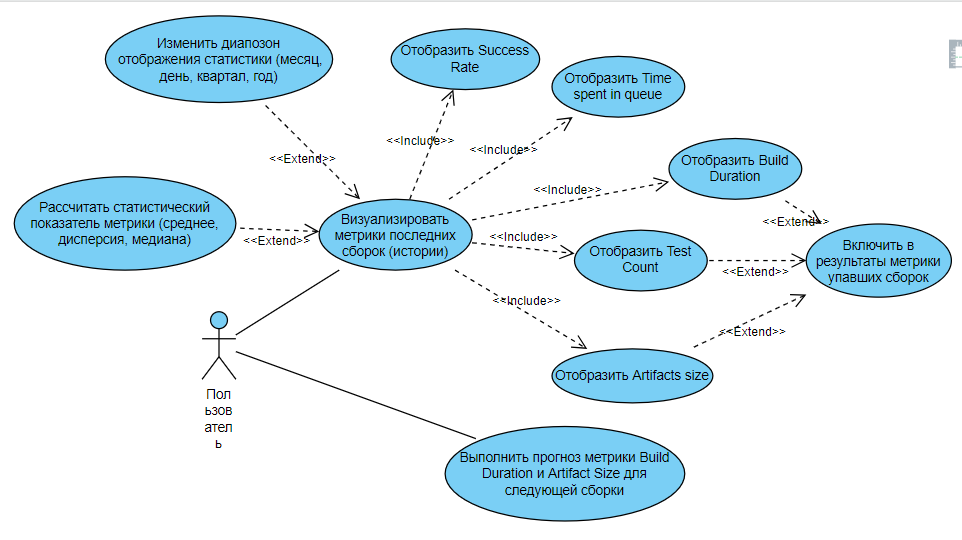
\includegraphics [scale=0.7] {my_folder/images//usecase3}
	\caption{Use case } 
	\label{fig:usecase3}  
\end{figure}

Функциональная модель в нотации IDEF0 отображена на рис.2.2. Декомпозиция процесса отображена в приложении П5.1-2 Основное внимание на диаграмме уделяется визуализации статистики сборок, поскольку это изначально является целью разработки. Также там будут отражены дополнительные функции такие как фильтрация, и высчитывание статистик метрик.

\begin{figure}[ht!] 
	\center
	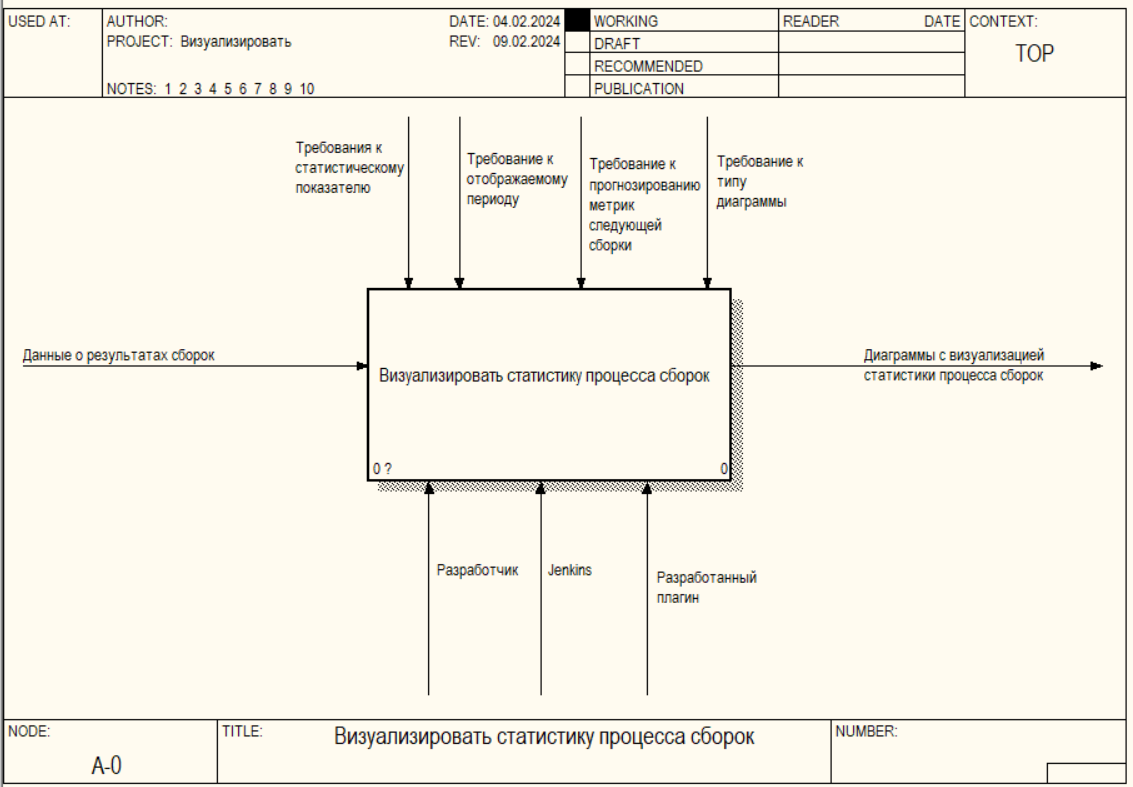
\includegraphics [scale=0.7] {my_folder/images//ide1_2}
	\caption{Процесс визуализации сборок} 
	\label{fig:er1}  
\end{figure}

\section{Архитектура Jenkins} \label{ch1:sec2}

Перед объяснением построения архитектуры плагинов Jenkins, необходимо привести схему архитектуры Jenkins, где будет отображено место разрабатываемых плагинов в CI системе. Архитектура Jenkins представлена на рис.2.3. Установленные плагины Jenkins-CI, а также локальные сценарии и приложения выполняются на сервере Jenkins-CI и предоставляют расширяемый набор функций управления и обработки данных \cite{article}.

\begin{figure}[ht!] 
	\center
	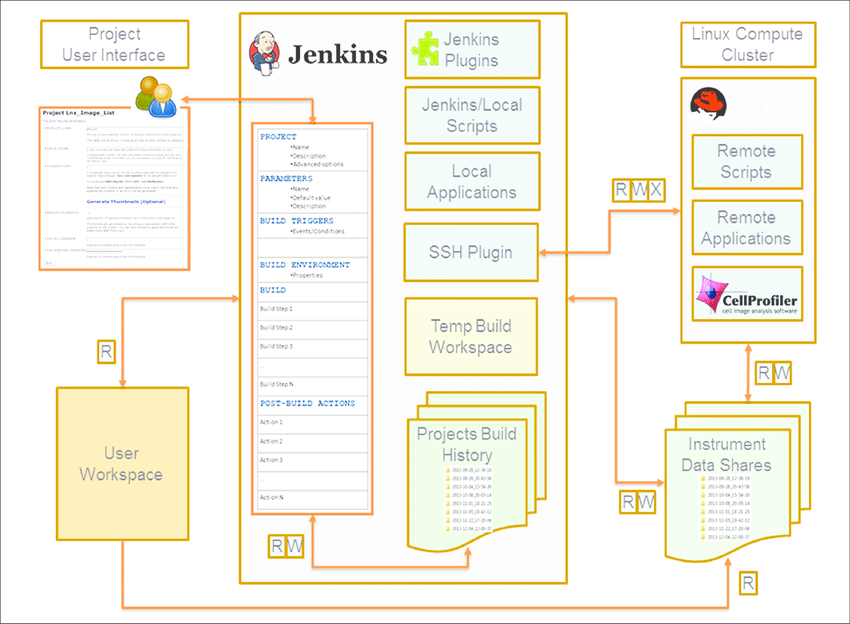
\includegraphics [scale=0.47] {my_folder/images//ArchitectureJenkins}
	\caption{Архитектура Jenkins \cite{article}} 
	\label{fig:ArchitectureJenkins}  
\end{figure}


Архитектура плагинов использует точки расширения, которые, предоставляют разработчикам плагинов возможности реализации для расширения функциональности системы Jenkins \cite{atchplugin}. Точки расширения автоматически обнаруживаются Jenkins во время загрузки системы.

В разрабатываемом плагине реализация будет происходить через класс Action. Actions являются основным строительным блоком расширяемости в Jenkins: их можно прикреплять ко многим объектам модели, хранить вместе с ними и при необходимости добавлять в их пользовательский интерфейс.

Помимо класса Action для того чтобы создать временные действия, которые будут прикреплены к заданию Jenkins будет использован класс TransientActionFactory, который позволяет создавать действия, которые будут отображаться на страницах Jenkins только при наличии соответствующего объекта - задания.

Разработка будет выполняться в объектно-ориентированной парадигме, т.е. приложение будет разбито на классы, будет применяться наследование, полиморфизм и инкапсуляция. Все классы, которые будут разработаны для плагина отображены на рис.2.4. 

\begin{figure}[ht!] 
	\center
	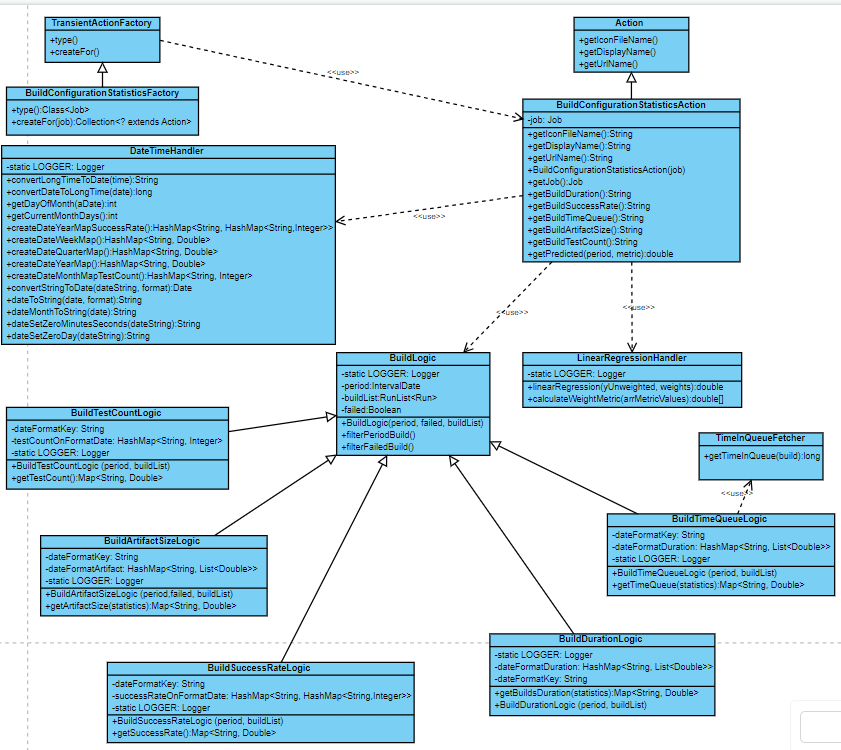
\includegraphics [scale=1] {my_folder/images//class3}
	\caption{Диаграмма классов плагина} 
	\label{fig:class3}  
\end{figure}

При рассмотрении диаграммы необходимо отметить, что два класса являются встроенными в Jenkins, это TransientActionFactory, который позволяет добавлять действия к любому типу объекта, а также интерфейс Action - добавленный к объекту модели, создает дополнительное подпространство URL-адресов под родительским объектом модели, через которое он может взаимодействовать с пользователями. Actions также способны открывать доступ к левому меню в интерфейсы Jenkins, по которому обычно производится навигация при конфигурировании сборки.

Для удобства использования плагина, предполагается добавить дополнительную ссылку в меню слева, для перехода на страницу визуализации метрик, а также динамически обновлять страницу при изменении параметров и фильтров, что и обосновывает использование данных встроенных классов.

Основная часть остальных классов требуется для работы с определенной метрикой статистики выполнения сборок Jenkins, что следует из их названия. Также будет разработан дополнительный класс DateTimeHandler, который позволит создать методы для удобной работы с датой и временем, что необходимо поскольку будет производиться преобразования одних типов дат к другим, сравнение дат между собой, а также получение определенных частей дат.

\section{Архитектура плагина} \label{ch1:sec3}

Для того чтобы визуализировать и обработать данные о сборках, необходимо получить эти данные. Для этого необходимо использовать различные методы и классы Jenkins, такие как Job - для работы с проектом (статическая сущность), а также Run для работы со сборкой (конкретные запуски Job, со временем выполнения и результатом). Внутри методов этих сущностей при их вызове будет отправляться API запрос на сервер Jenkins, который будет возвращать данные из хранилища xml файлов для каждой конкретной сборки.

После получения данных в плагине, идет их обработка и подготовка структур данных для визуализации. Вызов методов обработки данных о сборках будут происходить из Jelly файлов, в которых с помощью специальных тегов будет производиться связывание между объектами бизнес-логики Java и JS файлами, где будут создаваться графики визуализации.

Jelly для получения данных из Java использует AJAX запросы, а затем полученные данные сохраняет в DOM структуре страницы плагина. Затем с помощью JS происходит получение данных о сборках из DOM структуры и отправка в методы построения графиков.

Все взаимодействие между Java, Jelly и JS происходит с помощью JSON структур, такое решение было принято ввиду удобства работы со структурой с помощью этих инструментов. На рис.2.5 представлено изображение архитектуры плагина.

\begin{figure}[ht!] 
	\center
	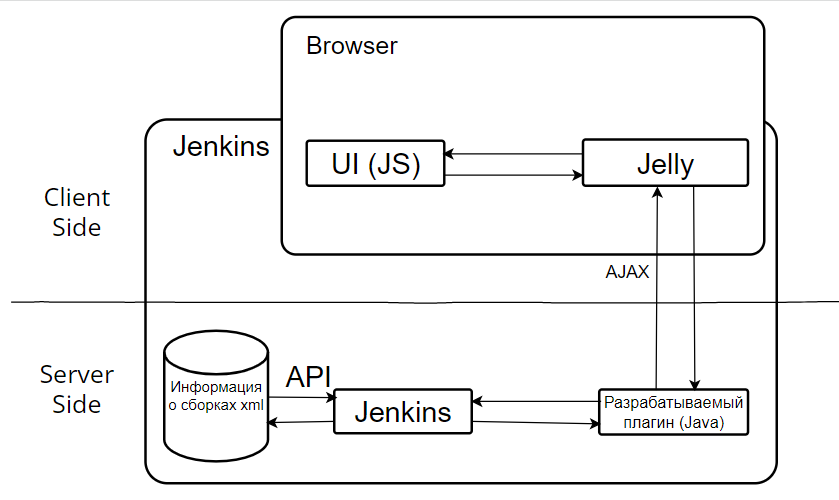
\includegraphics [scale=0.67] {my_folder/images//archpl3}
	\caption{Архитектура плагина} 
	\label{fig:ArchitecturePlugin}  
\end{figure}


\section{Языки программирования} \label{ch1:sec4}

Для программирования плагина будет использоваться язык Java. Поскольку Jenkins написан на Java, то все плагины необходимо писать на том же языке. Это является главным минусом, а возможно и сложностью при разработке плагинов на Jenkins, поскольку ограничивает свободу разработчика.

Есть возможность разработки плагина с использованием языка программирования Groovy. Groovy это динамический язык с возможностями статической типизации и статической компиляции для платформы Java \cite{groovy}, нацеленный на повышение производительности разработчиков, который плавно интегрируется с любой программой Java.

Недостатком такого выбора является то, что абсолютное большинство плагинов написано на чисто Java, а значит сообщества и поддержка при разработке на Java будет значительно большей. Также в сравнении с Groovy, Java обладает большей производительностью \cite{groovyvsjava}, статической типизацией и подходит для разработки приложений в парадигме ООП.

Java — это язык высокого уровня, который можно охарактеризовать следующими словами: объектно-ориентированный, многопоточный, динамический, высокопроизводительный и безопасный \cite{java}. Java используется для разработки высоконагруженных информационных систем, мобильных приложений, плагинов, десктопного ПО и др. К преимуществам Java также можно отнести компилируемость, что обеспечивает высокое быстродействие.

Java будет использоваться для программирования ядра плагина и бизнес-логики. Также для программирования графических компонентов, графиков и диаграмм будет использоваться язык программирования JavaScript. JS - это легковесный, интерпретируемый или JIT-компилируемый, объектно-ориентированный язык \cite{js}, основное предназначение которого выполнять сценарии на веб-страницах, что необходимо при разработке плагина, результаты которого отображаются на веб-страницах.

Помимо прочего, для стилизации компонентов веб-интерфейса будет использоваться язык каскадных таблиц стилей CSS \cite{css}, который позволит настроить удобное отображение и позиционирование элементов на странице плагина Jenkins. 

Верстка страниц будет осуществляться с помощью инструмента Jelly - все разрабатываемые плагины используют данный инструмент в Jenkins, поскольку с ним можно легко интегрировать Java, XML и JS. Jelly — это средство для преобразования XML в исполняемый код, это механизм сценариев и обработки на основе Java и XML \cite{jelly}. В Jelly можно вызывать функции Java, использовать такие синтаксические конструкции, как циклы, условия и переменные, также он позволяет легко обратиться к объектам в Java.

\section{Инструменты сборки} \label{ch1:sec5}

В качестве инструмента сборки проекта был выбран Maven, который можно использовать для создания и управления любым проектом на основе Java. Преимущества Maven были описаны в первой главе при рассмотрении инструментов сборок приложения.

Абсолютное большинство разработанных плагинов для Jenkins использует Maven, поскольку Maven предоставляет удобные архетипы для начала разработки плагинов, что делает использование того же Gradle не рациональным.


\section{Библиотеки} \label{ch1:sec6}

\subsection{Chart.js}

Поскольку проект предполагает использование графиков и диаграмм, то необходимо было выбрать инструмент для работы с графиками в Jenkins и Java, который позволит отображать графики прямо на странице задания Jenkins. В качестве этого инструмента была выбрана библиотека Chart.js, которая на данный момент является самой популярной JavaScript библиотекой по оценкам GitHub и загрузок npm \cite{chartjs}. К преимуществам данной библиотеки можно отнести: 
\begin{itemize}
	\item у Chart.js очень подробная документация;
	\item отрисовка canvas делает Chart.js очень производительным, особенно для больших наборов данных и сложных визуализаций;
	\item строит отзывчивый интерфейс - перерисовывает диаграммы при изменении размера окна для идеальной детализации масштаба.
\end{itemize}

\subsection{Gson}

Для удобства разработки и взаимодействия клиентской части с серверной необходимо, чтобы обработанные данные из Jenkins в браузер передавались в формате JSON. Для обеспечения преобразования объектов и структур Java в JSON была использована библиотека Gson от компании google. К важным особенностям и преимуществам данной библиотеки можно отнести:

\begin{itemize}
	\item легкость в использовании;
	\item отсутствие требования размещения аннотаций Java в пользовательских классах \cite{gson};
	\item поддержка Java Generics.
\end{itemize}

\subsection{Apache Commons Math}

Поскольку одним из требований к плагину является работа с математической статистикой для обработки метрик сборок, а также прогнозирование значений метрик, то необходима библиотека, которая реализует данный функционал. В качестве такой библиотеки была выбрана Apache Commons Math. Commons Math это библиотека легких, автономных математических и статистических компонентов, решающая наиболее распространенные проблемы \cite{commath}, связанные со статистикой. Преимущества использования библиотеки:

\begin{itemize}
	\item скорость математических вычислений выше, чем у стандартных средств Java;
	\item открытый исходный код;
	\item функции для статистической обработки и анализа данных (линейная регрессия).
\end{itemize}

\subsection{Junit}

Для того чтобы, протестировать разработанный плагин, будут написаны unit тесты. Поскольку разработка плагина будет вестись на языке Java, то для написания тестов будет использована Java инструмент. В качестве такого инструмента был выбран Junit, который состоит из следующих компонентов:  JUnit Platform, JUnit Jupiter, JUnit Vintage \cite{junit}. Основными преимуществами инструмента являются:

\begin{itemize}
	\item популярность и большое сообщество;
	\item использование для написания тестов Java (без дополнительных фреймворков и языков);
	\item совместимость с Java инструментами (Maven, Gradle).
\end{itemize}

\subsection{Mockito}

Поскольку функционал плагина использует обращение к структурам Jenkins (Job, Run), для тестирования необходимо использовать заглушки этих структур. Для работы с заглушками была выбрана библиотека mockito, которая была выбрана из-за следующих особенностей, причин и преимуществ:

\begin{itemize}
	\item сообщество StackOverflow назвало Mockito лучшим фреймворком для заглушек на Java \cite{mockito};
	\item входит в число 10 лучших библиотек Java среди всех библиотек;
	\item позволяет писать читабельные тесты, использовать BDD подход.
\end{itemize}

\section{Выводы} \label{ch1:sec7}

В данной главе было проведено проектирование плагина, составлена use-case диаграмма и диаграмма классов, построена функциональная модель системы, описана архитектура Jenkins, а также описана архитектура, разрабатываемого плагина. Затем были выбраны инструменты разработки плагина.


%% Вспомогательные команды - Additional commands
%
%\newpage % принудительное начало с новой страницы, использовать только в конце раздела
%\clearpage % осуществляется пакетом <<placeins>> в пределах секций
%\newpage\leavevmode\thispagestyle{empty}\newpage % 100 % начало новой страницы	         	 % Глава 2
\chapter{Реализация прототипа плагина} \label{ch3}

% не рекомендуется использовать отдельную section <<введение>> после лета 2020 года
%\section{Введение. Сложносоставное название первого параграфа первой главы для~демонстрации переноса слов в содержании} \label{ch1:intro}
В 3 главе будут рассмотрены и описаны основные классы, которые были разработаны в соответствии с диаграммой классов из приложения 1, а также полученные результаты.

\section{Описание разработанных классов} \label{ch3:sec1}

В процессе написания кода плагины были запрограммированы классы в соответствии с диаграммой классов из приложения 1.

\subsection{BuildConfigurationStatisticsAction}

Основной класс приложения, который реализует интерфейс действия, через этот класс происходит взаимодействие с Jelly, а также вызов всех остальных методов бизнес-логики плагина, и определены поля для работы со сборками, все методы для получения информации о конкретной метрике сборки помечены аннотацией @JavaScript для того, чтобы можно было их вызывать через JS в Jelly, также во всех этих методах тип возвращаемого объекта приведен к JSON, который и передается в DOM страницы плагина при взаимодействии с элементами пользовательского интерфейса.

В классе реализованы только одно закрытое поле job, с помощью которого происходит взаимодействие со сборкой в проекте, а также обработка выполненных запусков. А также следующие методы:

\begin{itemize}
	\item BuildConfigurationStatisticsAction(Job job) - конструктор класса;
	\item String getIconFileName() - метод, определяющий иконку приложения в боковом меню;
	\item String getDisplayName() - метод, определяющий отображаемое имя плагина в боковом меню и других частях страницы;
	\item String getUrlName() - метод, определяющий url, по которому доступна страница плагина;
	\item Job getJob() - метод-геттер для получения текущей сборки;
	\item String getBuildDuration(String period, String fail, String average) - метод для получения информации о времени продолжительности запусков сборки, за определенный период, с заданными настройками;
	\item String getBuildSuccessRate(String period) - метод для получения информации о проценте успешности выполнения запусков сборки, за определенный период;
	\item String getBuildArtifactSize(String period, String fail, String average) - метод для получения информации о созданных артефактов запусков сборки, за определенный период, с заданными настройками;
	\item String getBuildTestCount(String period, String fail) - метод для получения информации о количестве выполненных тестов при запуске сборки, за определенный период, с заданными настройками;
	\item String getBuildTimeQueue(String period, String average) - метод для получения информации о времени нахождения в очереди запусков сборки, за определенный период, с заданными настройками.
\end{itemize}

\subsection{DateTimeHandler}

Статический класс, созданный для взаимодействия с датами и их обработки при создании структур данных, которые также создаются в рамках этого класса, формирования структуры данных зависит от метрики и от периода за который нужно получить информацию.

В классе определено поле Logger LOGGER, с помощью которого записываются логи плагина. Также в классе определены методы:

\begin{itemize}
	\item Date convertLongTimeToDate(long time) - метод, преобразующей время в миллисекундах, прошедших с 1970 года, в дату типа Date;
	\item long convertDateToLongTime(Date date) - метод, преобразующей дату в миллисекунды, прошедшие с 1970 года;
	\item int getDayOfMonth(Date aDate) - метод, получающий номер дня из даты в месяце;
	\item int getLastMonthDays() - метод для получения дней в прошлом месяце;
	\item String dateToString(Date date, String format) - метод для преобразования типа Date, в строку в соответствии с заданным форматом даты;
	\item String dateMonthToString(Date date) - метод для преобразования типа Date, в строку в соответствии с форматом "yyyy-MM";
	\item String dateSetZeroMinutesSeconds(String dateString) - метод для обнуления минут и секунд в строке с датой;
	\item HashMap<String, Double> createDateMonthMap() - метод, создающий начальную структуру данных за прошедший месяц по дням, где в качестве значений словаря используются нули;
	\item HashMap<String, Double> createDateAllMap(RunList<Run> runs) - метод для создания начальной структуры данных, за весь прошедший период, который вычисляет на какие равные интервалы следует разбить общий промежуток времени, от создания первой сборки, до создания последней сборки;
	\item HashMap<String, Double> createDateDayMap() - метод, создающий начальную структуру данных за прошедший день по часам, где в качестве значений словаря используются нули;
	\item HashMap<String, HashMap<String,Integer>> createDateDayMapSuccess() - метод, создающий начальную структуру данных за прошедший день по часам, для вычисления процента успешности выполнения сборок, где в качестве значений словаря используется словарь, в котором записано сколько запусков сборки выполнено успешно, а сколько с ошибками;
	\item HashMap<String, HashMap<String,Integer>> createDateWeekMapSuccessRate() - метод, создающий начальную структуру данных за прошедшую неделю по дням, для вычисления процента успешности выполнения сборок, где в качестве значений словаря используется словарь, в котором записано сколько запусков сборки выполнено успешно, а сколько с ошибками;
	\item HashMap<String, HashMap<String,Integer>> createDateMonthMapSuccessRate() - метод, создающий начальную структуру данных за прошедший месяц по дням, для вычисления процента успешности выполнения сборок, где в качестве значений словаря используется словарь, в котором записано сколько запусков сборки выполнено успешно, а сколько с ошибками;
	\item HashMap<String, HashMap<String,Integer>> createDateQuarterMapSuccessRate() - метод, создающий начальную структуру данных за прошедший квартал по месяцам, для вычисления процента успешности выполнения сборок, где в качестве значений словаря используется словарь, в котором записано сколько запусков сборки выполнено успешно, а сколько с ошибками;
	\item HashMap<String, Integer> createDateMonthMapTestCount() - метод, создающий начальную структуру данных за прошедший месяц по дням, для вычисления количества выполненных тестов во время запуска сборки, где в качестве значений словаря используется целочисленные нули;
	\item HashMap<String, Integer> createDateDayMapTestCount() - метод, создающий начальную структуру данных за прошедший день по часам, для вычисления количества выполненных тестов во время запуска сборки, где в качестве значений словаря используется целочисленные нули;
	\item HashMap<String, Integer> createDateYearMapTestCount() - метод, создающий начальную структуру данных за прошедший год по месяцам, для вычисления количества выполненных тестов во время запуска сборки, где в качестве значений словаря используется целочисленные нули;
	\item HashMap<String, Integer> createDateQuarterMapTestCount() - метод, создающий начальную структуру данных за прошедший квартал по месяцам, для вычисления количества выполненных тестов во время запуска сборки, где в качестве значений словаря используется целочисленные нули;
	\item HashMap<String, Integer> createDateWeekMapTestCount() - метод, создающий начальную структуру данных за прошедшую неделю по дням, для вычисления количества выполненных тестов во время запуска сборки, где в качестве значений словаря используется целочисленные нули;
	\item HashMap<String, Double> createDateYearMap() - метод, создающий начальную структуру данных за прошедший год по месяцам, где в качестве значений словаря используются дробные нули;
	\item HashMap<String, Double> createDateQuarterMap() - метод, создающий начальную структуру данных за прошедший квартал по месяцам, где в качестве значений словаря используются дробные нули;
	\item HashMap<String, Double> createDateWeekMap() - метод, создающий начальную структуру данных за прошедшую неделю по дням, где в качестве значений словаря используются дробные нули;
	\item HashMap<String, HashMap<String,Integer>> createDateYearMapSuccessRate() - метод, создающий начальную структуру данных за прошедший год по месяцам, для вычисления процента успешности выполнения сборок, где в качестве значений словаря используется словарь, в котором записано сколько запусков сборки выполнено успешно, а сколько с ошибками.
\end{itemize}
	
	\subsection{IntervalDate}
	
	Перечисляемый тип для удобства работы с датами-периодами. Содержит следующие предопределенные константы:
	
	\begin{itemize}
	\item DAY - день;
	\item WEEK - неделя;
	\item MONTH - месяц;
	\item YEAR - год;
	\item QUARTER - квартал;
	\item ALL - константа для определения, того что будут вычисляться равные периоды для данных за все время, от начального запуска сборки до конечного.
\end{itemize}

\subsection{TimeInQueueFetcher}

Класс отвечающий за расчет времени, которая сборка провела в очереди перед тем как отправилась на выполнение. В классе определен один метод long getTimeInQueue(Run build) с помощью которого вычисляется нахождение времени в очереди в миллисекундах для конкретного запуска сборки.

\subsection{BuildLogic}
	
Базовый класс бизнес-логики, от которого наследуются все остальные более специфичные классы по каждой метрике, в классе определяются методы фильтрации по периоду и наличию упавших сборок в итоговых результатах. В классе определены следующие поля:

\begin{itemize}
	\item IntervalDate period - период за который производится отбор запусков сборок для дальнейшей обработки и визуализации;
	\item RunList<Run> buildList - список запусков у конкретной сборки;
	\item Boolean failed - поле, которое определяет нужно ли учитывать при обработке и визуализации упавшие сборки (true - надо учитывать);
	\item Logger LOGGER - поле, с помощью которого записываются логи плагина при выполнении методов класса.
\end{itemize}

Также в классе определены методы, которые наследуются всеми остальными классами бизнес-логики, которые отвечают за работу с определенной метрикой:

\begin{itemize}
	\item BuildLogic(IntervalDate period, Boolean failed, RunList<Run> buildList) - конструктор класса;
	\item void filterPeriodBuild() - метод, который производит отборок только тех запусков, которые удовлетворяют заданному периоду;
	\item void filterFailedBuild() - метод, который производит отборок только тех запусков, которые удовлетворяют полю failed, т.е. в зависимости от значения флага, либо включает в выборку упавшие сборки, либо нет.
\end{itemize}

\subsection{BuildArtifactSizeLogic}

Класс для работы с метрикой AS, в нем происходит пересчет параметров в зависимости от периода и настроек подданных на вход, а также высчитывается размер артифакта в Кб. В классе определены следующие поля:

\begin{itemize}
	\item HashMap<String, Double> dateFormatArtifact - структура данных для работы с запусками сборки относительно метрики AS, ключи даты за выбранный период, значения размер артефактов, созданных во время запуска за выбранный период;
	\item String dateFormatKey - поле, которое определяет формат даты за выбранный период, по которому будет происходить обработка и визуализация;
	\item Logger LOGGER - поле, с помощью которого записываются логи плагина при выполнении методов класса.
\end{itemize}

Также в классе определены методы:

\begin{itemize}
	\item BuildArtifactSizeLogic(IntervalDate period, Boolean failed, RunList<Run> buildList) - конструктор класса;
	\item Map<String, Double> getArtifactSize(Boolean average) - метод, в котором происходит фильтрация данных запусков сборок по периоду и флагу failed, определение формата дат и вычисление размера артефактов в Кб, а также расчет по статистической величине (например, среднее арифметическое), в зависимости от заданных настроек.
\end{itemize}

\subsection{BuildDurationLogic}

Класс для работы с метрикой BD, в нем происходит пересчет параметров в зависимости от периода и настроек подданных на вход, а также высчитывается продолжительность сборки в секундах. В классе определены следующие поля:

\begin{itemize}
	\item HashMap<String, Double> dateFormatDuration - структура данных для работы с запусками сборки относительно метрики BD, ключи даты за выбранный период, значения время выполнения запусков сборки за выбранный период;
	\item String dateFormatKey - поле, которое определяет формат даты за выбранный период, по которому будет происходить обработка и визуализация;
	\item Logger LOGGER - поле, с помощью которого записываются логи плагина при выполнении методов класса.
\end{itemize}

Также в классе определены методы:

\begin{itemize}
	\item BuildDurationLogic(IntervalDate period, Boolean failed, RunList<Run> buildList) - конструктор класса;
	\item Map<String, Double> getBuildsDuration(Boolean average) - метод, в котором происходит фильтрация данных запусков сборок по периоду и флагу failed, определение формата дат и вычисление времени выполнения запусков сборок, а также расчет по статистической величине (например, среднее арифметическое), в зависимости от заданных настроек.
\end{itemize}

\subsection{BuildSuccessRateLogic}

Класс для работы с метрикой SR, в нем происходит пересчет параметров в зависимости от периода, а также высчитывается процент успешности выполненных сборок за заданный промежуток времени. В классе определены следующие поля:

\begin{itemize}
	\item HashMap<String, HashMap<String,Integer>> successRateOnFormatDate - структура данных для работы с запусками сборки относительно метрики SR, ключи даты за выбранный период, значения процент успешности выполнения запусков сборки за выбранный период;
	\item String dateFormatKey - поле, которое определяет формат даты за выбранный период, по которому будет происходить обработка и визуализация;
	\item Logger LOGGER - поле, с помощью которого записываются логи плагина при выполнении методов класса.
\end{itemize}

Также в классе определены методы:

\begin{itemize}
	\item BuildSuccessRateLogic(IntervalDate period, RunList<Run> buildList) - конструктор класса;
	\item Map<String, Double> getSuccessRate() - метод, в котором происходит фильтрация данных запусков сборок по периоду, определение формата дат и вычисление процента успешности выполнения запусков сборок.
\end{itemize}

\subsection{BuildTestCountLogic}

Класс для работы с метрикой TS, в нем происходит пересчет параметров в зависимости от периода и настроек подданных на вход, а также высчитывается количество выполненных тестов во время работы сборок за определенный период. В классе определены следующие поля:

\begin{itemize}
	\item HashMap<String, Integer> testCountOnFormatDate - структура данных для работы с запусками сборки относительно метрики TS, ключи даты за выбранный период, значения количество выполненных тестов запусков сборки за выбранный период;
	\item String dateFormatKey - поле, которое определяет формат даты за выбранный период, по которому будет происходить обработка и визуализация;
	\item Logger LOGGER - поле, с помощью которого записываются логи плагина при выполнении методов класса.
\end{itemize}

Также в классе определены методы:

\begin{itemize}
	\item BuildTestCountLogic(IntervalDate period, RunList<Run> buildList) - конструктор класса;
	\item Map<String, Integer> getTestCount() - метод, в котором происходит фильтрация данных запусков сборок по периоду и флагу failed, определение формата дат и вычисление количества выполненных тестов в процессе исполнения запусков сборки.
\end{itemize}

\subsection{BuildTimeQueueLogic}

Класс для работы с метрикой TQ, в нем происходит пересчет параметров в зависимости от периода и настроек подданных на вход, а также высчитывается время ожидание сборки в очереди в миллисекундах. В классе определены следующие поля:

\begin{itemize}
	\item HashMap<String, Double> dateFormatDuration - структура данных для работы с запусками сборки относительно метрики TQ, ключи даты за выбранный период, значения время нахождения в очереди запусков сборки за выбранный период;
	\item String dateFormatKey - поле, которое определяет формат даты за выбранный период, по которому будет происходить обработка и визуализация;
	\item Logger LOGGER - поле, с помощью которого записываются логи плагина при выполнении методов класса.
\end{itemize}

Также в классе определены методы:

\begin{itemize}
	\item BuildTimeQueueLogic(IntervalDate period, RunList<Run> buildList) - конструктор класса;
	\item Map<String, Double> getTimeQueue(Boolean average) - метод, в котором происходит фильтрация данных запусков сборок по периоду и флагу failed, определение формата дат и вычисление времени нахождения в очереди запусков сборок, а также расчет по статистической величине (например, среднее арифметическое), в зависимости от заданных настроек.
\end{itemize}

\subsection{Файлы JS и Jelly}

В JS определяются функции событий для выбора элемента из выпадающего списка и взаимодействия с флажками. Для каждой метрики используется своя функции, внутри определяются настройки данных и отображения для визуализации отдельной метрики в виде определенного графика/диаграммы, вызывается метод для сортировки агрегированных по датам значений метрик в структуре JSON, а также формируются метки-подписи для каждого типа периода.

Также в JS определены следующие функции:

\begin{itemize}
	\item formatLabelsDate(arrLabels, dateFormat, period) - функция, в которой происходит формирование меток-подписей к графикам в зависимости от формата дат и выбранного периода;
	\item sortOnKeys(dict, period) - функция в которой происходит сортировка значений словаря с данными о запусках сборок по ключам-датам;
	\item createSuccessRateChart(period) - функция в которой происходит подготовка данных, формирование настроек и создание графика по метрике SR;
	\item createTestCountChart(period) - функция в которой происходит подготовка данных, формирование настроек и создание графика по метрике TC;
	\item createBuildDurationChart(period) - функция в которой происходит подготовка данных, формирование настроек и создание графика по метрике BD;
	\item createArtifactSizeChart(period) - функция в которой происходит подготовка данных, формирование настроек и создание графика по метрике AS;
	\item createTimeQueueChart(period) - функция в которой происходит подготовка данных, формирование настроек и создание графика по метрике TQ.
\end{itemize}

В jelly файле с помощью html формируется структура документа, а также выполняется привязка Java объектов к объектам JS. Определяются обработчики событий, который при взаимодействии с пользователем вызывают определенный запрос-метод AJAX.

\section{Результаты разработки плагина} \label{ch3:sec2}

При разработке плагина надо было учитывать, что требуется отображать все графики на одной странице задания друг под другом, поскольку при выборе одно периода, например, месяца, будет получена сводная информация по каждой сборке или нескольких сборок запущенных в один день. Графики отображаются посредством переходна на соответствующую ссылку, оставляя при этом пользователя в том же задании (странице с результатами последних сборок).

В интерфейсе у каждого графика были реализованы те дополнительные функции отображения, которые могут быть применены к визуализируемой метрике: отобразить статистику по упавшим сборкам/тестам, усреднить метрику.

Интерфейс страницы плагина с графиками в системе Jenkins на странице задания показан на рисунке 3.1.


\begin{figure}[ht!] 
	\center
	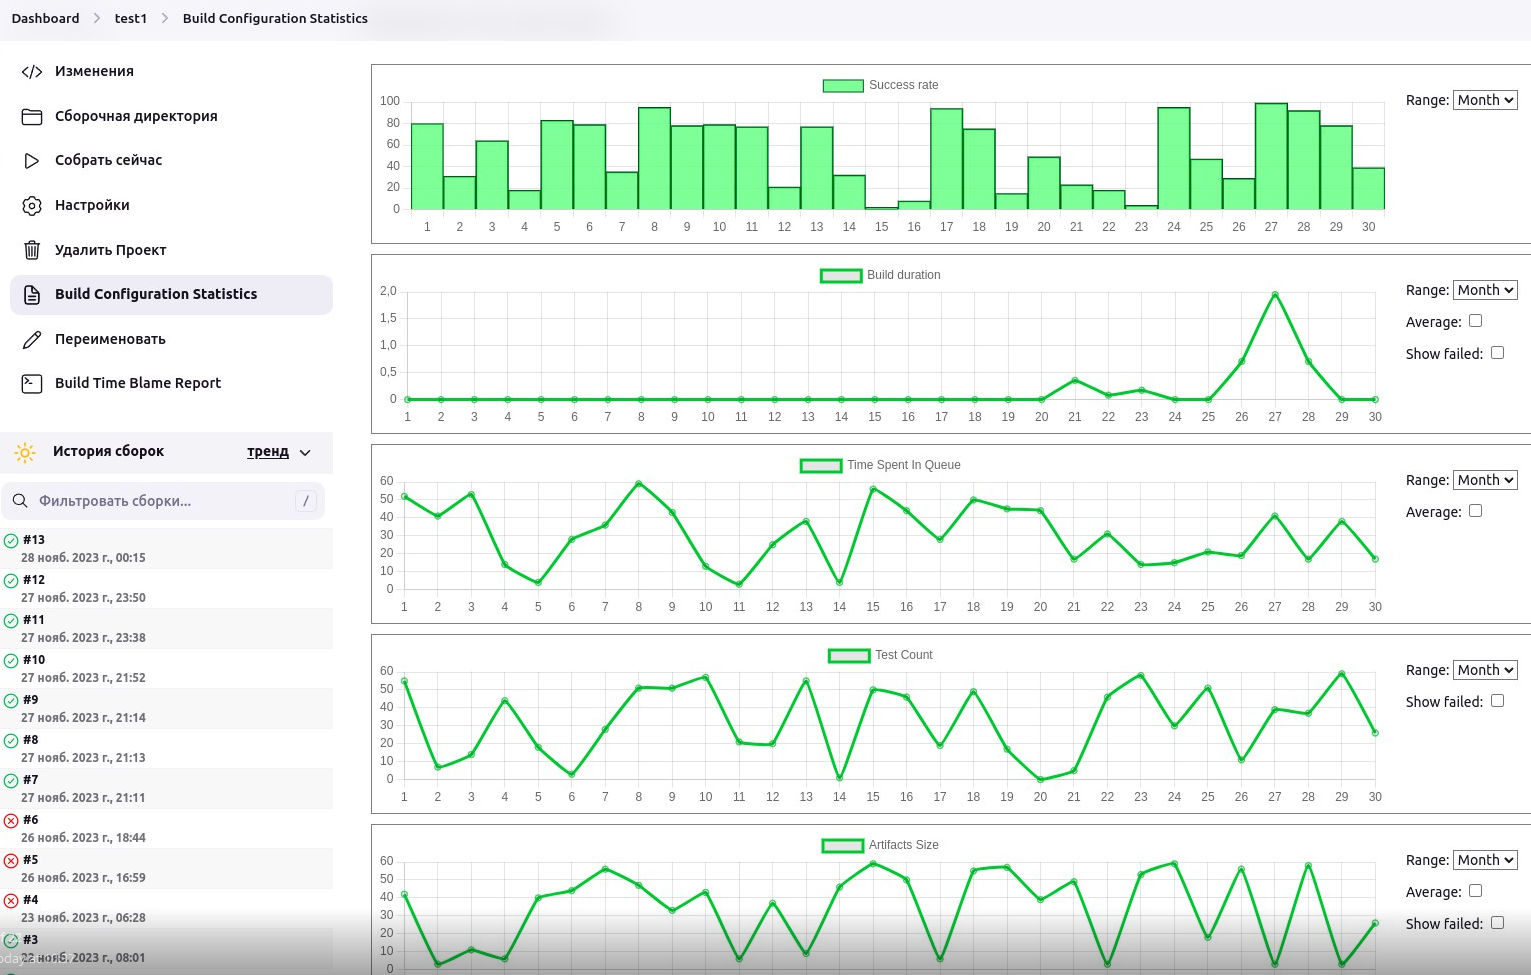
\includegraphics [scale=0.47] {my_folder/images//ui}
	\caption{Интерфейс плагина Jenkins} 
	\label{fig:ArchitectureJenkins}  
\end{figure}

Интерфейс страницы плагина с графиками в системе Jenkins на странице задания при выборе всех включенных настроек, а также с выбранным периодом неделя показан на рисунке 3.2.

\begin{figure}[ht!] 
	\center
	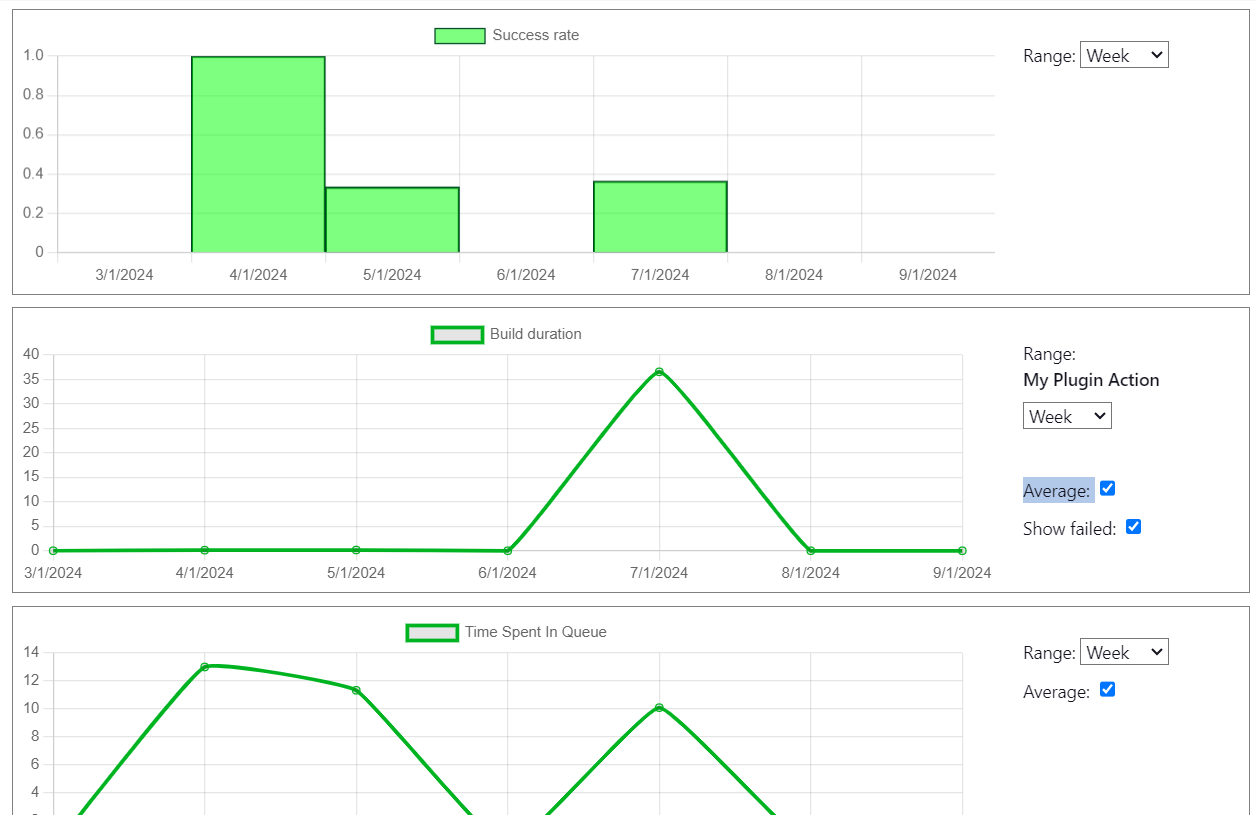
\includegraphics [scale=0.47] {my_folder/images//ui4}
	\caption{Интерфейс графиков с включенным настройками и периодом неделей} 
	\label{fig:ArchitectureJenkins}  
\end{figure}

Основное взаимодействие с графиками будет производить через меню, которое есть напротив каждого графика со своими параметрами, отображенном на рисунке 3.3:

\begin{figure}[ht!] 
	\center
	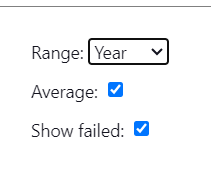
\includegraphics [scale=0.47] {my_folder/images//ui2}
	\caption{Интерфейс элементов управления} 
	\label{fig:ArchitectureJenkins}  
\end{figure}

При взаимодействии с раскрывающимся списком должен вызываться Java метод, который пересчитает и отфильтрует необходимые сборки Jenkins и динамически отобразит результаты по выбранными периоду, также динамически должна производить обработка метрик сборок, при выборе основной метрики ни как суммы всех значений, а как среднего, а также включение в графики данных об упавших сборках, при выборе соответствующих чекбоксов.

Интерфейс изменения навигационной панели отображен на рисунке 3.4. В данном случае видно что изменения видны при открытии конфигурации конкретной сборки, т.е. не надо будет переключаться между окном плагина и сборкой для визуализации метрик, при открытии данного пункта меню, также происходит изменения URL, с которым в дальнейшем и происходит взаимодействие.

\begin{figure}[ht!] 
	\center
	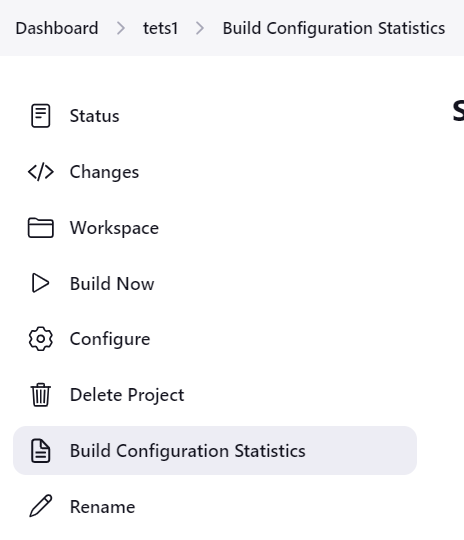
\includegraphics [scale=0.47] {my_folder/images//ui3}
	\caption{Интерфейс элементов управления} 
	\label{fig:ArchitectureJenkins}  
\end{figure}


Код плагина представлен в приложении 4.
 
\section{Выводы} \label{ch3:sec3}

В главе 3 была проведена реализация плагина, а также описаны классы, разработанные при написании плагина и файлы, которые участвуют во взаимодействии с этими классами и отображаемым интерфейсом пользователя. Также были приведены результаты разработки, приведены скриншоты интерфейсов, а также описаны добавленные на страницу Jenkins элементы, после установки плагина.





%
%

%
%
%\begin{table} [htbp]% Пример оформления таблицы
%	\centering\small
%	\caption{Представление данных для сквозного примера по ВКР \cite{Peskov2004}}%
%	\label{tab:ToyCompare}		
%		\begin{tabular}{|l|l|l|l|l|l|}
%			\hline
%			$G$&$m_1$&$m_2$&$m_3$&$m_4$&$K$\\
%			\hline
%			$g_1$&0&1&1&0&1\\ \hline
%			$g_2$&1&2&0&1&1\\ \hline
%			$g_3$&0&1&0&1&1\\ \hline
%			$g_4$&1&2&1&0&2\\ \hline
%			$g_5$&1&1&0&1&2\\ \hline
%			$g_6$&1&1&1&2&2\\ \hline		
%		\end{tabular}	
%	\normalsize% возвращаем шрифт к нормальному
%\end{table}


% \firef{} от figure reference
% \taref{} от table reference
% \eqref{} от equation reference




           	 % Глава 3
\chapter{Тестирование и апробация плагина в Jenkins} \label{ch4}

% не рекомендуется использовать отдельную section <<введение>> после лета 2020 года
%\section{Введение. Сложносоставное название первого параграфа первой главы для~демонстрации переноса слов в содержании} \label{ch1:intro}

В главе описано проведенное тестирование и апробация плагина:

\begin{enumerate}
	\item Описаны методы тестирования.
	
	\item Проведена апробация плагина в системе Jenkins.
	
	\item Разработан код тестирования плагина.
	
	
	
\end{enumerate}

\section{Методы тестирования} \label{ch4:sec1}

Тестирование программного обеспечения — обширное понятие, которое включает планирование, проектирование и, собственно, выполнение тестов  \cite{testing}. В процессе CI/CD производится непрерывное тестирование разработанного кода, а также тестирование разработанного приложения. Сам плагин является частью CI/CD процессе, но также требует тестирования корректной работы своей функциональности, тестирование разработанного кода, а также тестирования на соответствие исходным требования, которые были предъявлены к разработке в главе 1.

Существует множество методов тестирования и техник тест дизайна, в процессе анализ функциональных требования были отобраны те, которые наиболее релевантные для разработанного плагина Jenkins.

Будет проведено как ручное, так и автоматизированное тестирование плагина. Ручное тестирование поможет выявить нетипичные тест-кейсы, которые не покрываются автоматизированными тестами.

Ручные тесты будут проведены методом черного ящика. Данный метод это процедура получения и выбора тестовых случаев на основе анализа функциональности и технического задания, без применения знаний о внутреннем устройстве системы \cite{blacktest}.

Были составлены тест-кейсы, которые отражены в таблице 4.1.

\begin{table}
    \centering
    \caption{Составленные тест-кейсы}
    \begin{tabular}{|p{1cm}|p{5cm}|p{9cm}|}
    \hline
        № & Описание & Ожидание  \\ \hline
        1 & Проверка выбранного периода на графике SR (месяц) & Количество  дней соответствует прошлому месяцу, на каждый день отображены корректные значения процента успешности сборок\\ \hline
        2 & Проверка выбранного периода на графике BD (неделя) с учетом выбора настройки среднего значения и  упавших сборок& Количество  дней 7 в соответствии со всеми днями недели, на каждый день отображены корректные значения среднего времени продолжительности сборок, учтены упавшие сборки \\ \hline
        3 & Проверка выбранного периода на графике TQ (квартал) с учетом выбора настройки среднего значения & Количество  кварталов 4 в соответствии с кварталами года, на каждый квартал отображены средние значения проведенного в очереди времени сборок  \\ \hline
        4 & Проверка выбранного периода на графике TC (год) с учетом выбора настройки упавших сборок & Количество  месяцев 12 соответствует прошедшему году, на каждый месяц отображены корректные значения  количества тестов, с учетом тестов выполненных на упавших сборках \\ \hline
        5 & Проверка выбранного периода на графике AS (день) & Количество  часов 24 соответствует всем часам прошедшего дня, на каждый час отображены корректные значения размера итоговых артефактов полученного по результатам задания   \\ \hline
        6 & Проверка корректного отображения при выборе периода ALL & Отображены сборки со всего периода прошедшего, информация поделена на равное части   \\ \hline
        7 & Проверка корректного отображения аномальных значений & Отображены номера сборок, возле каждого графика, у которых аномальное значений метрики соответствующей графику   \\ \hline
        8 & Проверка корректного расчета предугаданной 'следующей' сборки& Метрики предугаданной сборки рассчитываются корректно для каждого графика   \\ \hline

    \end{tabular}
\end{table}

В данном случае тест-кейсы были описаны с помощью техники тест-дизайна Матрица трассировки. Если обратиться к определению, то матрица трассировки — двумерная таблица, содержащая соответствие функциональных требований и подготовленных тестовых сценариев \cite{matrixtest}, а на пересечении столбцов и строк ставится метка, о том, что данное требование покрывается данным тест-кейсом. В случае данной работы из соображений удобства и оптимизации тестовой документации, было принято решение модифицировать матрицу трассировки и совместить с подробным описание в формате чек листа: для оптимизации идет проверка, что каждый тип графика-метрики (Success Rate) корректно себя ведет на определенном периоде (неделя), таким образом не придется проверять, каждый график на каждом периоде при каждой доработке кода продукта.

Данные тест-кейсы оптимизированы, поскольку в соответствии с пирамидой тестирования \cite{TestPyramid} ручные UI кейсы, находятся в самой верхней ее части и не должны занимать достаточно большое место в системе тестирования. С дрогой стороны для улучшения покрытия требования, предъявляемых к продукты должны использоваться гораздо в большем объеме unit-тесты, т.е. тесты в которых самые маленькие компоненты системы - модули (модули, классы, методы), индивидуально проверяются на предмет правильной работы \cite{unittest}.

\subsection{Unit тестирование}

При написание юнит тестов используется метод белого ящика. Данный метод предоставляет тестировщику полное знание тестируемого приложения, включая доступ к исходному коду и проектной документации \cite {whitebox}, т.е. тестирование происходит на основе знания исходного кода, таким образом, юнит тестирование методом белого ящика поможет нам достаточно широко покрыть все модули плагина. Для запуска тестов требуется перейти в корень директории плагина и выполнить команду mvn test.

Код юнит тестов расположен в классе BuildConfigurationStatisticsBuilderTest. В этом классе проводятся проверки, такие как:

\begin{itemize}
	\item проверка корректности системы в целом - testWorkingSystem();
	\item проверка успешного завершения сборки - testSuccessBuildFromCustomBuild();
	\item проверка падения сборки при некорректных входных данных - testFailBuildFromCustomBuild();
	\item проверка формирования структур для начальной инициализации данных - testCreateDateWeekMapSuccessRate(), testCreateDateMonthMap();
	\item проверки корректности написанных методов работы с датой - testDateMonthToString(), testGetLastMonthDays();
	\item проверка работоспособности модулей обработки времени сборок - testGetTimeInQueue().
\end{itemize}

Код юнит тестов приведен в приложении 5.

\subsection{UI тестирование}

Также для автоматизации тестирования UI части плагина, был применен Selenium web driver и язык программирования python. WebDriver управляет браузером, как это делает пользователь, с использованием сервера Selenium \cite{webdriver}. Данные тест-кейсы будут в автоматическом режиме проверять реакцию элементов веб интерфейса на действия пользователя. Для запуска тестов требуется перейти в корень проекта Selenium и запустить команду pytest, при необходимости указать браузер и url, с которыми необходимо запустить UI тесты.

Код UI тестов расположен в отдельном проекте в классе TestCase. В этом классе проводятся проверки, такие как:

\begin{itemize}
	\item проверка корректности открытия и наличия элементов во вкладке на странице плагина - test\_open\_tab(self);
	\item проверка наличия и корректного отображения графика SR - test\_success\_rate\_chart(self);
	\item проверка наличия и корректного отображения графика BD - test\_build\_duration\_chart(self);
	\item проверка наличия и корректного отображения графика TC - test\_test\_count\_chart(self);
	\item проверка наличия и корректного отображения графика BQ - test\_time\_spent\_queue\_chart(self);
	\item проверка наличия и корректного отображения графика AS - test\_artifacts\_size\_chart(self);
	\item проверка корректности реакция элемента выпадающего списка - test\_change\_value\_select\_period(self);
	\item проверка  корректности реакция чекбоксов - test\_change\_value\_checkbox(self).
\end{itemize}

Код UI тестов приведен в приложении 6.



 \section{Апробация плагина} \label{ch4:sec2}
 
 Апробация плагина будет проводится в системе CI Jenkins для которой и был разработан плагин визуализации. Для того чтобы провести апробацию плагина на локальном сервере Jenkins, запущенном на локальном или удаленном ПК, потребуется произвести несколько операций. Для начала, нужно будет клонировать репозиторий с кодом плагина на GitHub, перейти в папку проекта и выполнить \cite{deployplugin} Maven mvn install и скопировать .hpi в папку /plugins/. 
 
 Затем потребуется на запущенном сервере Jenkins перейти в Управление Jenkins  и среди доступных плагинов выбрать Build Configuration Statistics, установить, после чего напротив каждой сборки Jenkins в боком меню, откуда можно запустить и отредактировать сборку, появится пункт меню Build Configuration Statistics, при нажатии на которой должны отобразиться все графики с собранной статистикой по метрикам каждого задания в Jenkins. 
 
 \subsection{Подготовка и генерация набора сборок для апробации}
 
 Для того чтобы графики отображали какие-то данные, необходимо сначала сгенерировать сборки разной длительности, статусов, с разным количеством тестов и размером артефактов.
 
Для генерации запусков сборки, можно задать конфигурацию сборки через меню Configuration, а затем с помощью действия Build Now в меню сборки, запустить сборку на выполнение. Также можно использовать плагин Pipeline, для того чтобы декларативно с помощью groovy скрипта задать конфигурацию сборки с шагами, которые будут выполнять при запуске сборки. 

Пример скрипта для создания для создания сборки, в которой будет выполняться два шага: создание файла и создания артефакта сборки из созданного файла с помощью cmd Windows.

\begin{lstlisting}
pipeline {
    agent any
    stages {
        stage('Create file') {
            steps {
                bat 'echo Hello World > myfile.txt'
            }
        }
        stage('Archive file') {
            steps {
                archiveArtifacts artifacts: 'myfile.txt', onlyIfSuccessful: true
            }
        }
    }
}
\end{lstlisting}

Для того чтобы проверить корректность обработки данных во времени, можно после запуска сборки, отредактировать (в логах выбранного запуска в папке запуска в файле build.xml) xml теги   <timestamp>1684077728000</timestamp> и
  <startTime>1684077728013</startTime> , в которых в формате timestamp задать нужное время в прошлом. Для конвертации даты и времени в timestamp можно использовать веб-ресурс https://www.epochconverter.com/.
  
Например, для даты Sunday, May 14, 2023 3:22:08 PM получаем следующий результат в формате timestamp 1684077728000 в миллисекундах. После редактирования xml файла с информацией о сборке получим необходимое дату  и время в интерфейсе Jenkins. Пример отредактированной сборки с датой в прошлом указан на рисунке 4.1.

 \begin{figure}[ht!] 
	\center
	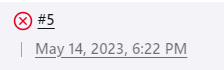
\includegraphics [scale=0.87] {my_folder/images//lastBuild}
	\caption{Сборка с датой в прошлом} 
	\label{fig:lastBuild}  
\end{figure}
 
 В ходе апробации плагина были сгенерированы сборки, которые отображены на рисунке 4.2.
 
 \begin{figure}[ht!] 
	\center
	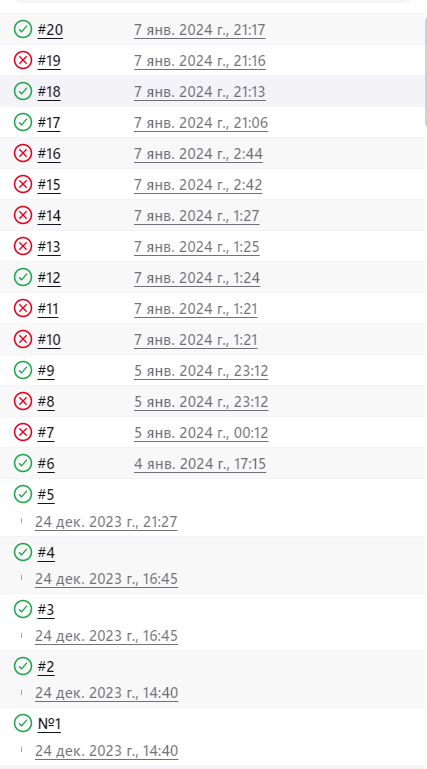
\includegraphics [scale=0.47] {my_folder/images//builds}
	\caption{Сгенерированные сборки} 
	\label{fig:builds}  
\end{figure}

Запуски были сгенерированы с разной датой начала:

\begin{itemize}
	\item 5 успешных запусков с датой 24.12.2023, с разным временем начала с 2 до 9 часов вечера;
	\item 1 успешный запуск 4.01.2024;
	\item 3 запуска 5.01.2024 - 2 из которых закончилось с результатом падение (в 0 часов и 23 часа), а один с положительным результатом в 23 часа;
	\item 11 запусков 7.01.2024 из которых 7 закончилось падением, а 4 с успешным результатом, запуски имеют разное время начала с 1 до 21 часа ;
	\item 2 запуска 11.01.2024 один из которых закончился падением с временем начала 14 часов, а другой с успешным результатом в 14 часов;
	\item 2 успешных запуска 12.01.2024 со временем начала 13 часов и 16 часов.
\end{itemize}


 Среди сборок присутствуют, упавшие сборки со специально завышенным временем выполнения 100 секунд, сборки без завышенного времени выполнялись около 20 секунд. Такая сборка отображена на рисунке 4.3.
 
 \begin{figure}[ht!] 
	\center
	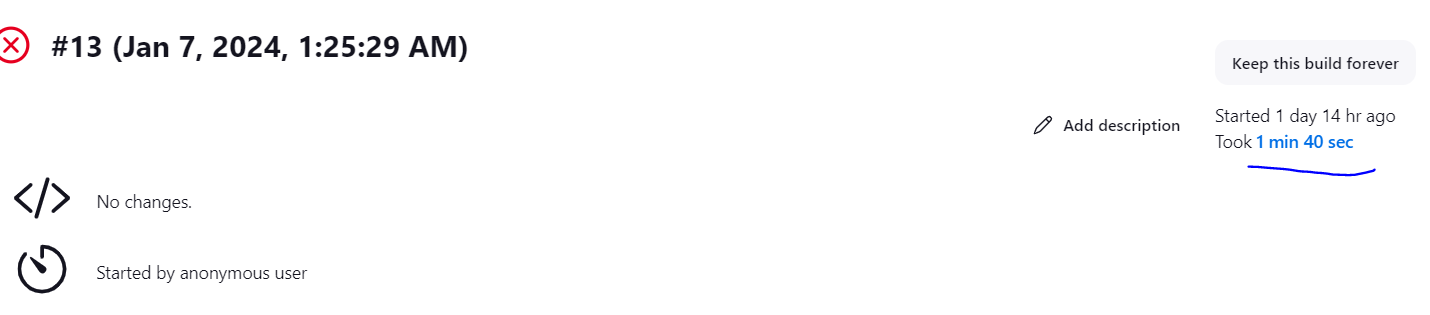
\includegraphics [scale=0.47] {my_folder/images//longBuild}
	\caption{Длинная упавшая сборка} 
	\label{fig:longBuild}  
\end{figure}


А также сборки, с созданными артефактами, часть из которых в статусе успешного выполнения, с короткой продолжительностью, а часть из которых завершены падением с большой продолжительностью выполнения. Были определены разные файлы-артефакты для генерации с размером от 70 байт до 1 Кб. Перенос созданных файлов в артефакты выполнялся с помощью конфигурационного разделы в сборке Post-build Actions, в котором выплавлялась команда Archive the artifacts. Сборка с артефактом отображена на рисунке 4.4.
 
 \begin{figure}[ht!] 
	\center
	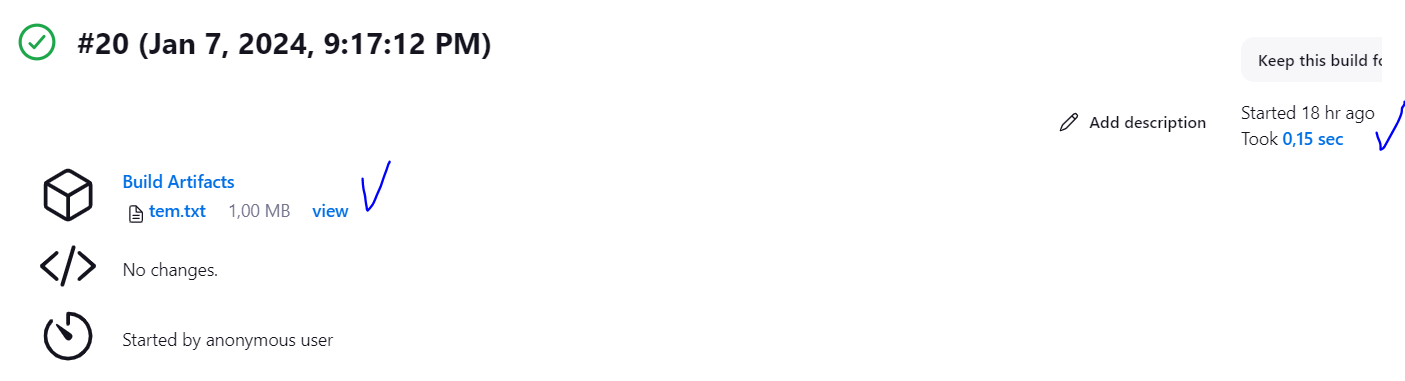
\includegraphics [scale=0.47] {my_folder/images//artifactBuild}
	\caption{Короткая успешная сборка с артефактом} 
	\label{fig:artifactBuild}  
\end{figure}



Часть сборок выполнялось посредством созданного класса в плагине BuildConfigurationStatisticsBuilder, который добавлял еще один вариант запуска шагов сборки Build Steps. Этот класс выполнял вывод информации о текущес запуске в консоль, а также вывод информации с именами всех запусков, уже выполненных в сборке, а также вывод параметра, который задавался при создании шага в конфигурации сборки. Информация из консоли с процессом выполнения шага представлена на рисунке 4.5.

 \begin{figure}[ht!] 
	\center
	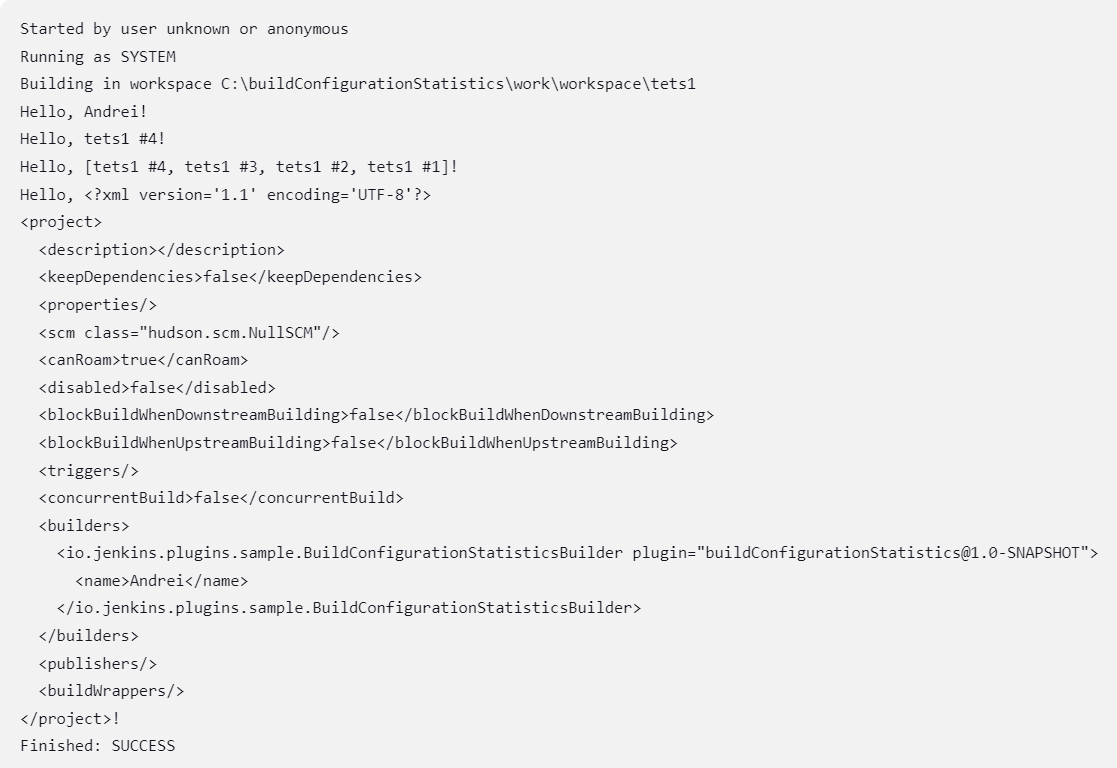
\includegraphics [scale=0.57] {my_folder/images//console1}
	\caption{Консоль шага с разработанным Builder} 
	\label{fig:customBuilder}  
\end{figure}



Для части сборок был добавлен 1 шаг с выполнением cmd команды  \textit{echo 123}, для создания упавших сборок, команды cmd намеренно прописывались с ошибками в синтаксисе, например  \textit{echo1 123}.

Для того чтобы увеличить время выполнения сборок использовалась команда cmd  \textit{waitfor SomethingThatIsNeverHappening /t 100  2>NUL}, которая обеспечивала время выполнения запуска 100 секунд.

Для создания небольших файлов-артефактов использовалась команда cmd \textit{echo "tempbuild1111111111111111111"  1>tembuild.txt}. А для генерация файлов в 1Кб команда \textit{fsutil file createnew tem.txt 1048576}.

\subsection{Апробация на проекте с открытым исходным кодом}

Для того, чтобы убедиться, что плагин работает также на уже существующих проектах, необходимо провести апробацию на стороннем проекте. В качестве такого проекта был выбран frontend-maven-plugin (https://github.com/eirslett/frontend-maven-plugin). 

Это плагин, который загружает/устанавливает Node и NPM локально для вашего проекта, запускает npm install, а затем любую комбинацию Bower , Grunt , Gulp , Jspm , Karma или Webpack и может работать в Windows, OS X и Linux \cite{frontplugin}. У проекта 865 forks на GitHub, а также более 4 тысяч звезд, из чего следует, что его разработка была полезна для ИТ сообщества и активно используется разработчиками.

Следуя, указаниям из документации для сборки проекта необходимо вызвать команду \textit{mvn clean install}. В случае тестирования разработанного плагина  в системе Jenkins, также использовался ключ -l, который сохранит логи сборки проекта в отдельный файл clean. Также в настройках сборки Jenkins было настроено действие после сборки для создания артефакта из полученных логов.

Для моделирования ситуации просмотра статистики по метрикам сборки в условиях разных версий продукта, когда вносятся значительные изменения в код, что влечет за собой увеличния, в возможно и уменьшения (в случаи оптимизации) времени сборки продукта, необходимо откатиться к более ранним коммитам. Поскольку для апробации используется открытый проект, то данные манипуляции с исходным кодом возможно выполнить. Для того чтобы откатиться к предыдущим версиям, были проделаны следующие действия:

\begin{enumerate}
	\item Сделать fork проекта в личный репозиторий.
	
	\item Найти подходящий коммит, в котором были выполнены значительные изменения (более 500 строк измененного кода).
	
	\item Откатиться до найденного коммита.
	
	\item Создание новой ветки на основе коммита, до которого произошел откат.
	
	\item Отправка ветки в личный удаленный репозиторий на GitHub.
	
\end{enumerate}

После того как произведен откат до выбранного коммита, необходимо повторить процедуру начиная с коммита, до которого был произведен откат. Процедура была повторена 12 раз т.е. было сгенерировано 12 версий проекта на 12 месяцев года (для генерации сборок на год).

Для отката к более ранним версия был написан скрипт на языке Python, представленный в приложении П7.

Далее при генерации сборок было произведено по 2 запуска на каждую версию продукта, время в каждой сборке было отредактировано на каждый месяц за прошедший год. Перед выполнением каждого запуска был отредактирован параметр, по которому определяется из какой ветки берется исходный код продукта.

-----

Для проверки подсчета метрики TC, был добавлен второй шаг  \textit{mvn clean test}, который запускает юнит тесты, а также в разделе Post-build Actions добавлено действие Publish JUnit test result report, которое по результатам прогона теста формирует отчет JUnit из xml лога с результатами, созданного после выполнения всех тестов.

------

Сгенерированные на этом проекте сборки отображены на рисунке 4.6.

 \begin{figure}[ht!] 
	\center
	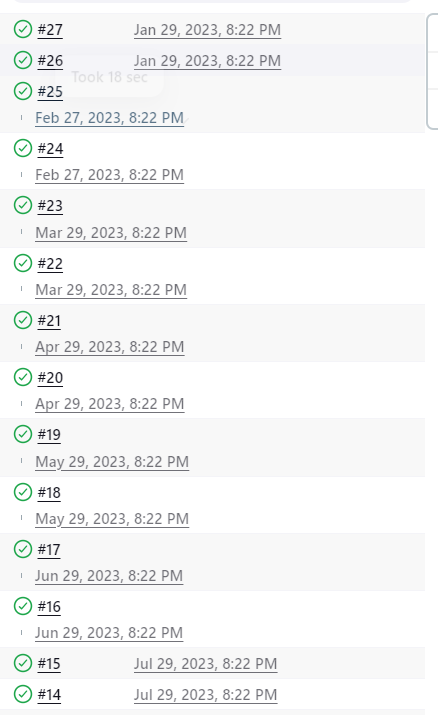
\includegraphics [scale=0.67] {my_folder/images//genetatedBuild}
	\caption{Сгенерированные сборки реального проекта} 
	\label{fig:genetatedBuild}  
\end{figure}

Результаты работы плагина на описанном выше проекте отображены на рисунках 4.7-8. На рисунке 4.7 видно на графике SR, как менялся процент успешности сборок в течении года на столбчатой диаграмме. Также видно на графике BD динамику изменения продолжительности сборок за последний год на линейном графике, в данном случае можно отследить как менялось среднее значение продолжительности. Видно, что время сборки незначительно увеличивалось, т.е. при увеличении кода приложения, в продолжительности сборки также увеличивалось время, за исключением 8 и 11 месяцев. 


 \begin{figure}[ht!] 
	\center
	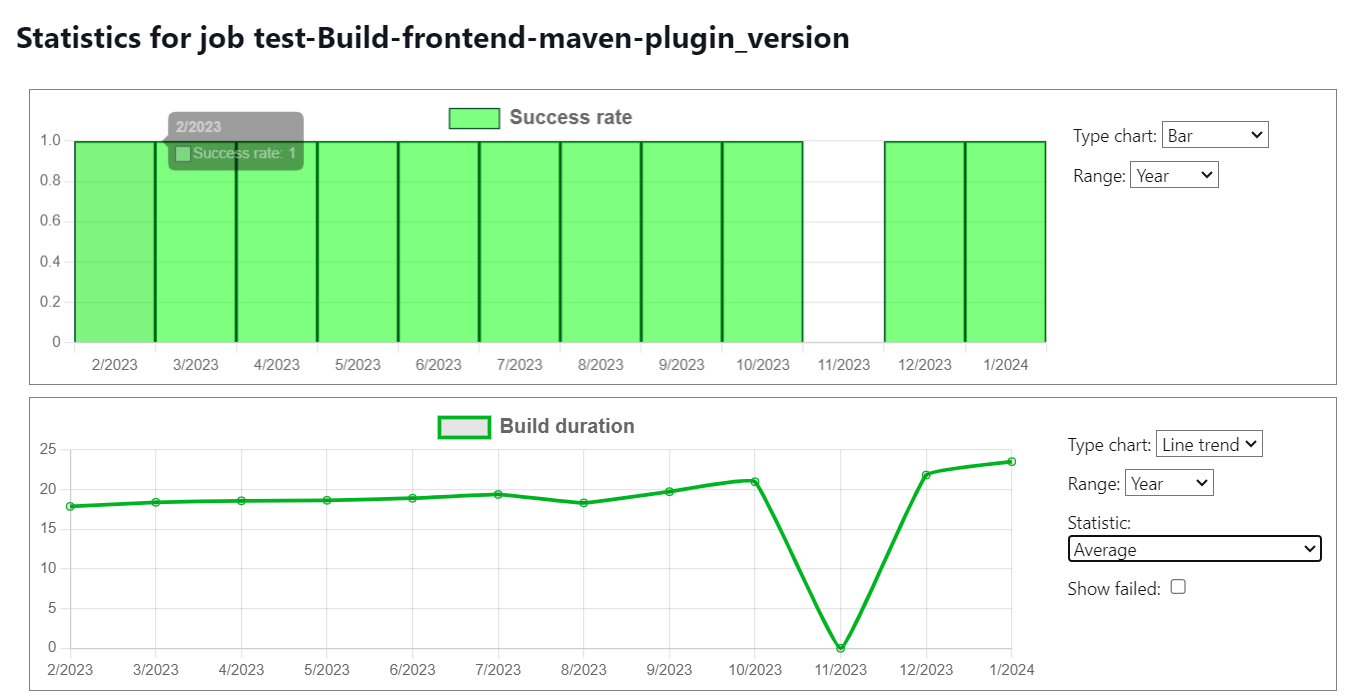
\includegraphics [scale=0.47] {my_folder/images//reares1}
	\caption{Результаты апробации на реальном проекте SR, BD} 
	\label{fig:reares1}  
\end{figure}

В 8 месяце в изменениях кода была повышена версия npm и node, что оптимизировало время выполнения сборки, которое уменьшилось с 19.3 до 18.3 секунд. А версия в 11 месяце, вероятно была не протестировано перед загрузкой в главную ветку, поскольку результат из 3 запусков сборки закончился падением. Что также видно на графике SR, т.е. можно сделать вывод что в коммите был дефект, а не оптимизация, которая ускорила время сборки в несколько раз.

На рисунке 4.8 можно увидеть с помощью радарной диаграммы общий размер, сгенерированных логов-артефактов за последний год. Видно, что с каждым месяцем размер артефактов увеличивался, что также можно объяснить увеличением исходного кода продукта, также наглядна видно разницу между первым и последним месяцем года, а также то что при отображении упавших сборок видно, то что генерировались артефакты, хоть и с небольшим размером.

 \begin{figure}[ht!] 
	\center
	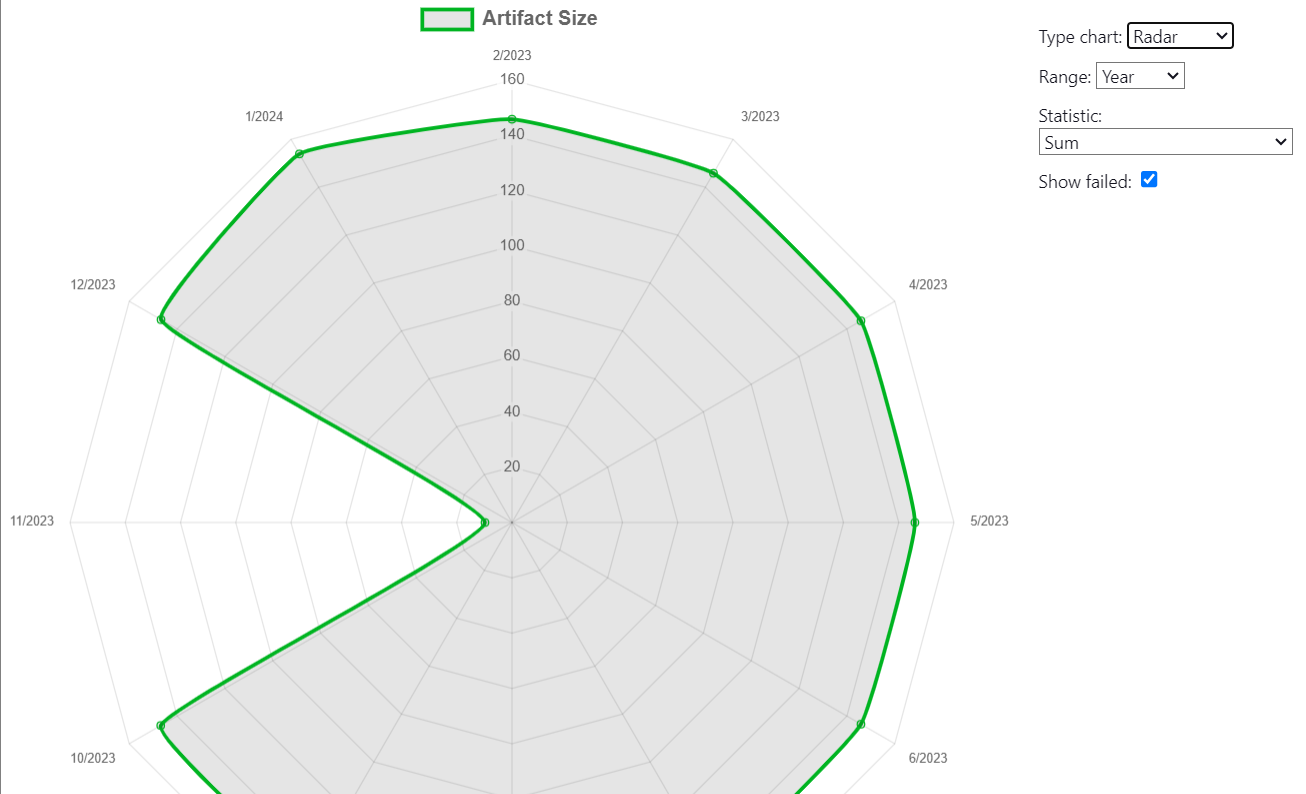
\includegraphics [scale=0.47] {my_folder/images//realres2}
	\caption{Результаты апробации на реальном проекте AS} 
	\label{fig:realres2}  
\end{figure}

По описанным выше результатам визуализации можно прийти к выводу, что плагин полезен тем, что отображает изменение различных метрик запусков сборки с течением времени, т.е. можно увидеть тенденцию изменений в созданных сборках Jenkins в течении цикла разработки за нужный период времени и если метрики в какой момент изменили свои значения, можно определить, что это за момент (или период) и проанализировать как изменения в сборке, тестах или коде могли повлиять на это.

Для удобства пользователей, как видно на рисунках выше, результаты отображаются на разных типах диаграмм, чтобы каждой участник команды мог изучать динамику изменения метрик, так как ему удобно. Также видно, что возле метрик BD, SR, AS можно выбрать статистический показатель, в соответствии с которым будут обработана метрика. Тем самым, можно определить является отклонение случайностью, нестабильностью сборки или это какая-то закономерность.

После анализа разработчики, тестировщики и DevOps-инженеры могут принять решение, насколько критичны данные изменения для процессов CI/CD и если потребуется оптимизировать сборки, тесты или, возможно, какую-то часть кода.

Также по данным диаграммам можно обнаружить и другие проблемы, например, аномалии в процессах сборки или тестирования или окружении, в котором производится сборка или установка компонентов системы.

 \subsection{Оценка результатов работы}
 
 Для того чтобы оценить результаты работы, будет проведено сравнение функционала, который присутствует в аналогичных решениях: плагинах, сравнительный анализ, которых проводился в разделе 1.5 и модуль Statistics, реализованный в средстве CI TeamCity, который и послужил причиной для создания аналогичного модуля в Jenkins.
 
 
 


В разработанном плагине реализовано 7 статистических показателей, которые применяются к метрикам сборок, что является значительным преимуществом в сравнении с аналогичными решениями, поскольку в аналогичных плагинах Jenkins, а также в модуле TeamCity реализован только расчет среднего арифметического значения, и при том не во всех аналогичных плагинах Jenkins.

Также преимуществом разработанного плагина является наличие 3 типов диаграмм для каждой метрики, что больше чем у всех аналогичных решений.

Все результаты сравнения с аналогичными решениями приведены в таблице 4.2.

 \begin{table}
    \centering
    \caption{Количественные результаты работы}
    \begin{tabular}{|p{3cm}|p{3cm}|p{2cm}|p{2cm}|p{2cm}|p{2cm}|}
    \hline
        Критерий & Разработанное решение & TeamCity & Build Monitor Plugin & Global Build Stats Plugin  & Build Time Blame \\ \hline
        Количество визуализируемых метрик & 5 & 5 & 1 & 2 &2 \\ \hline
        Количество статистических показателей & 7 & 1 & 0 & 1 &1\\ \hline
        Количество типов диаграмм & 3 & 2 & 1 & 1 &1\\ \hline


    \end{tabular}
\end{table}

Если сравнивать по количеству визуализируемых метрик, то видно, что все 5 метрик, которые были реализованы в TeamCity, удалось реализовать и в разработанном плагине, аналогичные плагины Jenkins визуализируют определенные из перечисленных в разделе 1.5 метрик, но их количество меньше 5.


 
 
\section{Выводы} \label{ch4:sec3}

После проведения этапа апробации и тестирования плагина визуализации статистики сборок Jenkins можно прийти к выводу, что тестирование проведено в полном объеме и затронуло разные методы, техники тест-дизайна и соответствует методологиям и устоявшимся практикам тестирования программного обеспечения. Апробация протестированного плагина, дала понять, что плагин корректно отрабатывает при разных поданных на вход исходных данных и настройках. Корректно высчитываются и визуализируются статистические показателе обработанных метрик:

\begin{itemize}
	\item среднее арифметическое;
	\item мода;
	\item медиана;
	\item размах;
	\item среднеквадратическое отклонение;
	\item среднеквадратическое отклонение несмещенное;
	\item дисперсия.
\end{itemize}

Визуализация метрик со статистическими показателями была проверена на различных типах диаграмм/графиков:

\begin{itemize}
	\item столбчатая диаграмма;
	\item линейный тренд;
	\item радарная диаграмма.
\end{itemize}

В результате разработки автоматизированных тестов было разработано 22 юнит теста и 8 UI тестов.






%
%

%
%
%\begin{table} [htbp]% Пример оформления таблицы
%	\centering\small
%	\caption{Представление данных для сквозного примера по ВКР \cite{Peskov2004}}%
%	\label{tab:ToyCompare}		
%		\begin{tabular}{|l|l|l|l|l|l|}
%			\hline
%			$G$&$m_1$&$m_2$&$m_3$&$m_4$&$K$\\
%			\hline
%			$g_1$&0&1&1&0&1\\ \hline
%			$g_2$&1&2&0&1&1\\ \hline
%			$g_3$&0&1&0&1&1\\ \hline
%			$g_4$&1&2&1&0&2\\ \hline
%			$g_5$&1&1&0&1&2\\ \hline
%			$g_6$&1&1&1&2&2\\ \hline		
%		\end{tabular}	
%	\normalsize% возвращаем шрифт к нормальному
%\end{table}


% \firef{} от figure reference
% \taref{} от table reference
% \eqref{} от equation reference




           	 % Глава 3
\ContinueChapterEnd % завершить размещение глав <<подряд>>
%% Завершение основной части

\chapter*{Заключение} \label{ch-conclusion}
\addcontentsline{toc}{chapter}{Заключение}	% в оглавление 

В результате проведенной работы был разработан прототип плагина для визуализации статистики сборок Jenkins. Была проанализирована предметная область, проведен сравнительный аналил аналогичных решений.

Были выбраны средства и инструменты разработки, спроектирована архитектура плагина, описаны функциональные возможности, а также разработан программный код и интерфейс плагина.

В процессе проектирования и реализация были выбраны статистические показатели и типы диаграм, по которым должна происходить визуализация метрик сборок Jenkins. Было проведено тестирование плагина различными методами и апроьация на реальном проекте.        	 % Заключение

%% Наличие следующих перечней не исключает расшифровку сокращения и условного обозначения при первом упоминании в тексте!
\input{my_folder/acronyms}		         % Необязательная рубрика! Список сокращений и условных обозначений



    		 % Необязательная рубрика! Словарь терминов
% По порядку после Списка сокращений и условных обозначений, если есть.	


%%% Не мянять - Do not modify
%%
%%


\clearpage                                  % В том числе гарантирует, что список литературы в оглавлении будет с правильным номером страницы
%\hypersetup{ urlcolor=black }               % Ссылки делаем чёрными
%\providecommand*{\BibDash}{}                % В стилях ugost2008 отключаем использование тире как разделителя 
\urlstyle{rm}                               % ссылки URL обычным шрифтом
\ifdefmacro{\microtypesetup}{\microtypesetup{protrusion=false}}{} % не рекомендуется применять пакет микротипографики к автоматически генерируемому списку литературы
%\newcommand{\fullbibtitle}{Список литературы} % (ГОСТ Р 7.0.11-2011, 4)
%\insertbibliofull  
%\noindent
%\begin{group}
\chapter*{Список использованных источников}	
\label{references}
\addcontentsline{toc}{chapter}{Список использованных источников}	% в оглавление 
\printbibliography[env=SSTfirst]                         % Подключаем Bib-базы
%\ifdefmacro{\microtypesetup}{\microtypesetup{protrusion=true}}{}
%\urlstyle{tt}                               % возвращаем установки шрифта ссылок URL
%\hypersetup{ urlcolor={urlcolor} }          % Восстанавливаем цвет ссылок










%\urlstyle{rm}                               % ссылки URL обычным шрифтом
%\ifdefmacro{\microtypesetup}{\microtypesetup{protrusion=false}}{} % не рекомендуется применять пакет микротипографики к автоматически генерируемому списку литературы
%\insertbibliofull                           % Подключаем Bib-базы
%\ifdefmacro{\microtypesetup}{\microtypesetup{protrusion=true}}{}
%\urlstyle{tt}                               % возвращаем установки шрифта ссылок URL
		     % Список литературы

% Здесь можно поместить список иллюстративного материала

\appendix % не редактировать / keep unmodified


%

\chapter{UML диаграмма классов плагина}
\begin{figure}[ht!] 
	\center
	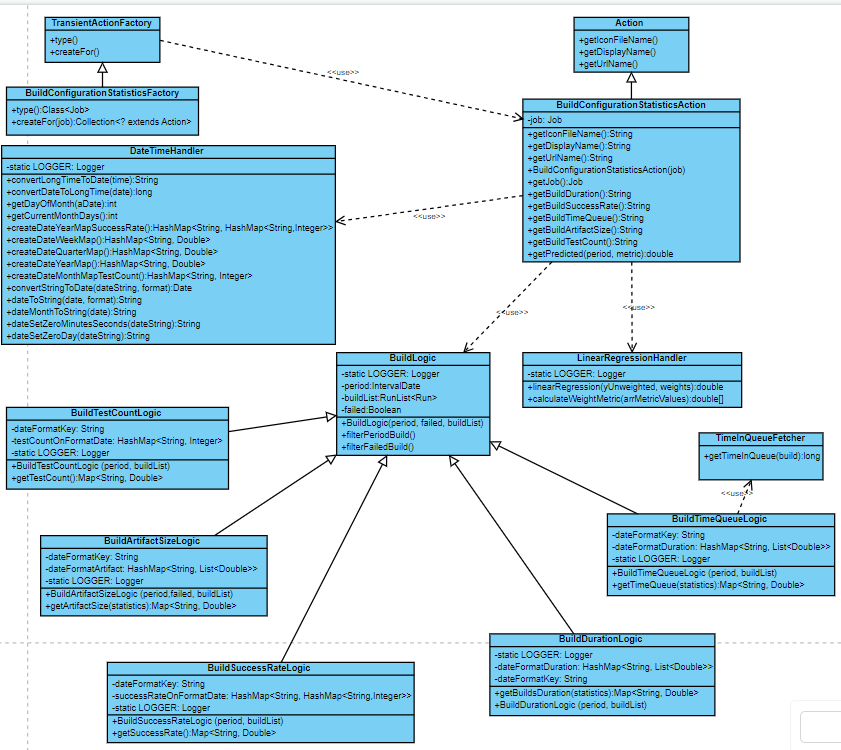
\includegraphics [scale=1] {my_folder/images//class3}
	\caption{Диаграмма классов плагина} 
	\label{fig:class3}  
\end{figure}



			     % Приложение 1

%\chapter{Idef0}\label{appendix-extra-examples}
\begin{figure}[ht!] 
	\center
	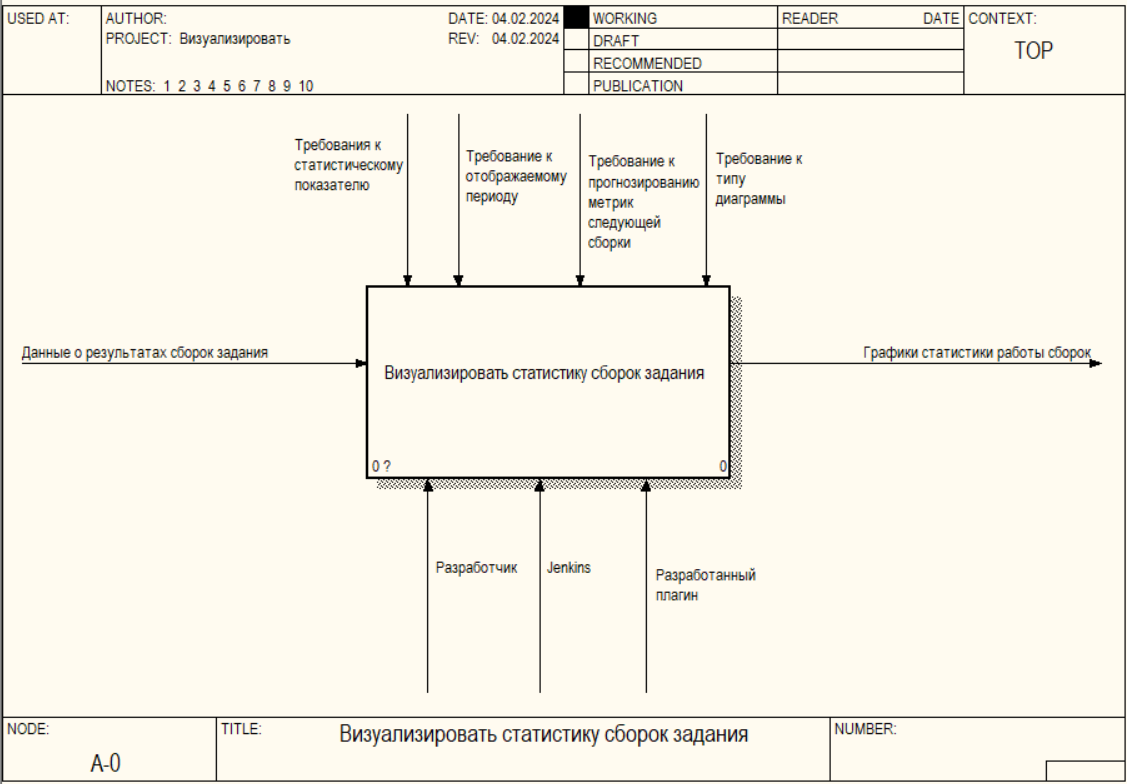
\includegraphics [scale=0.7] {my_folder/images//er1}
	\caption{Процесс визуализации сборок} 
	\label{fig:er1}  
\end{figure}

\begin{figure}[ht!] 
	\center
	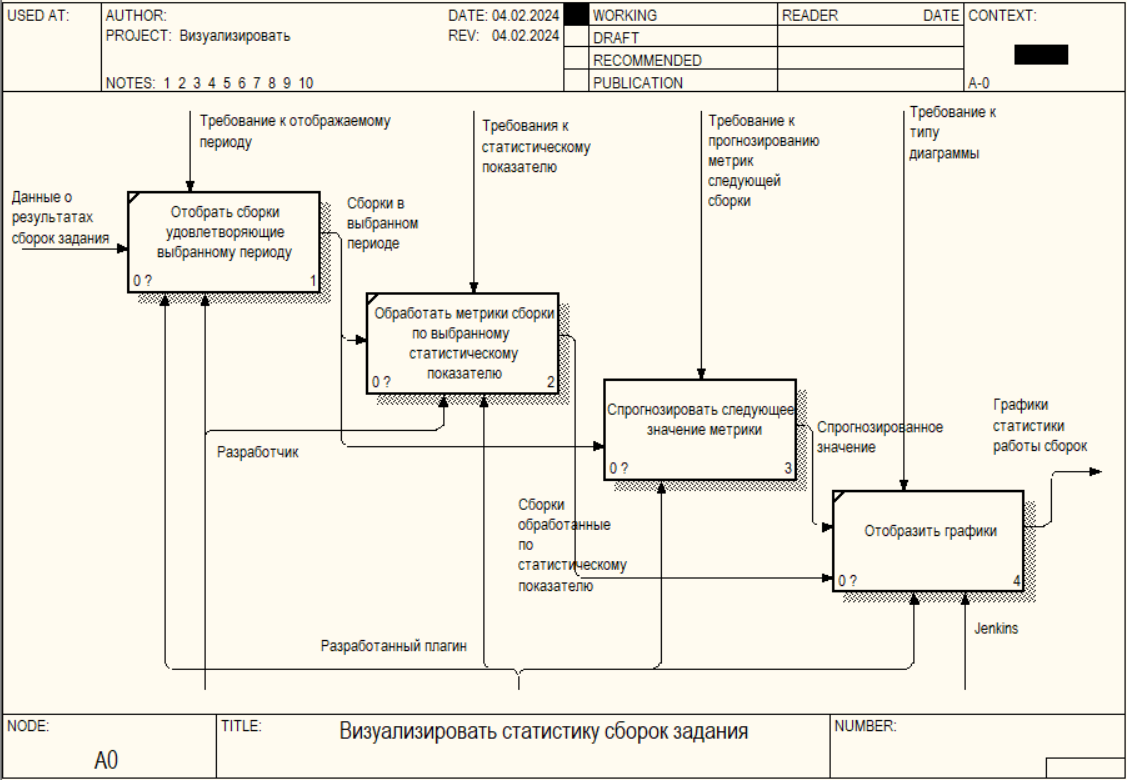
\includegraphics [scale=0.7] {my_folder/images//er2}
	\caption{Детализация процесса визуализации} 
	\label{fig:er2}  
\end{figure}

\begin{figure}[ht!] 
	\center
	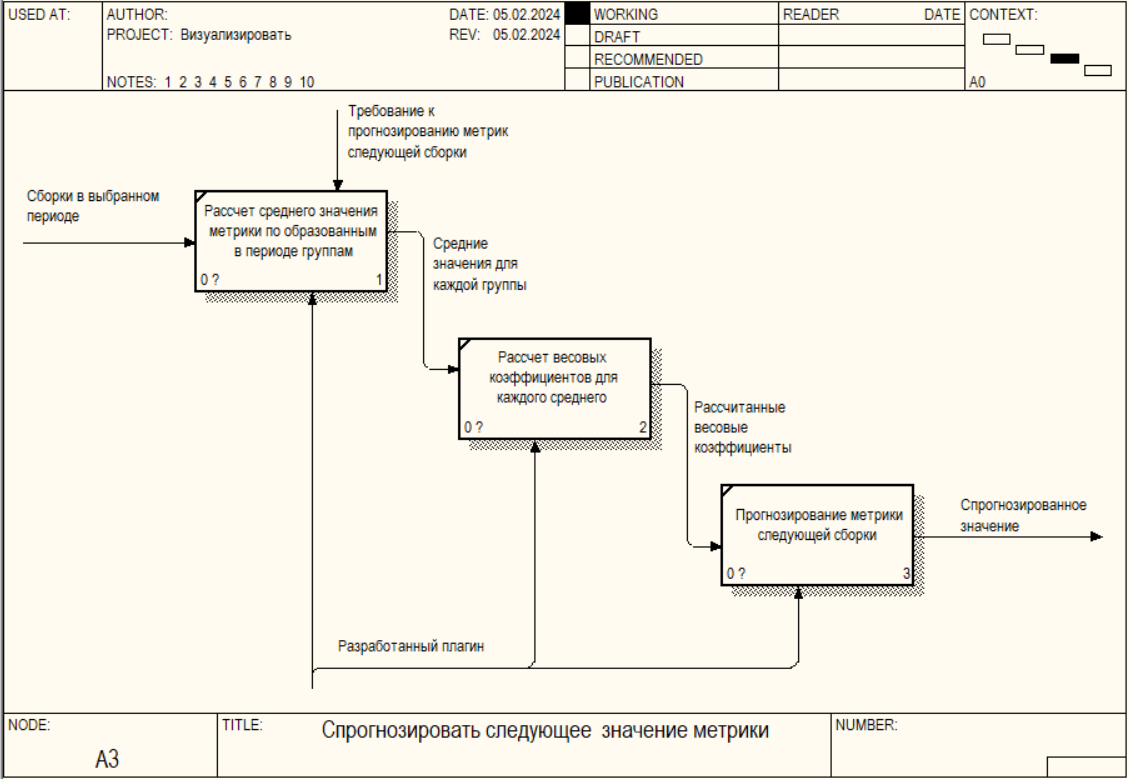
\includegraphics [scale=0.7] {my_folder/images//er3}
	\caption{Процесс прогнозирования метрики} 
	\label{fig:er3}  
\end{figure}

			 	 % Приложение 2

%\chapter{Use-case}\label{appendix-extra-examples}
\begin{figure}[ht!] 
	\center
	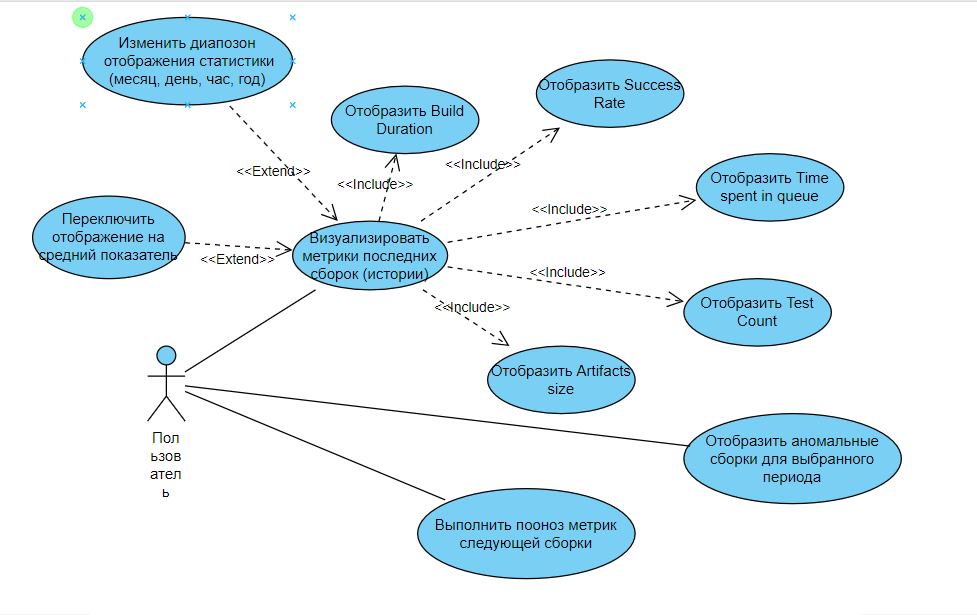
\includegraphics [scale=0.7] {my_folder/images//usecase2}
	\caption{Use case } 
	\label{fig:spbpu_hydrotower-app-}  
\end{figure}
			 	 % Приложение 2

\chapter{Программный код}\label{appendix-extra-examples}

\begin{lstlisting}[language=Java]
package io.jenkins.plugins.sample;

import hudson.model.Action;
import hudson.model.Job;
import jenkins.security.stapler.StaplerDispatchable;
import org.kohsuke.stapler.StaplerRequest;
import org.kohsuke.stapler.StaplerResponse;
import org.kohsuke.stapler.bind.JavaScriptMethod;
import org.kohsuke.stapler.interceptor.RequirePOST;

import javax.servlet.ServletException;
import java.io.IOException;
import java.text.ParseException;
import java.util.Map;
import java.util.logging.Level;
import java.util.logging.Logger;

public class BuildConfigurationStatisticsAction implements Action {



    private Job job;

    public BuildConfigurationStatisticsAction(Job job) {
        this.job = job;
    }

    @Override
    public String getIconFileName() {
        return "document.png";
    }

    @Override
    public String getDisplayName() {
        return "Build Configuration Statistics";
    }

    @Override
    public String getUrlName() {
        return "buildConfigurationStatistics";
    }

    public Job getJob() {
        return job;
    }

    public Map<String, Double> getBuildDuration(String period, String fail, String average) throws ParseException {
        Logger LOGGER = Logger.getLogger("uuu");
        LOGGER.log(Level.INFO, "arg jelly: " + period);
        LOGGER.log(Level.INFO, "failed status: " + fail);
        LOGGER.log(Level.INFO, "avg status: " + average);
        IntervalDate intreval = IntervalDate.valueOf(period);
        Boolean failed = fail.equals("1");
        Boolean averageTime = average.equals("1");
        return new BuildDurationLogic(intreval, failed,job.getBuilds()).getBuildsDuration(averageTime);
    }

    public Map<String, Double> getBuildSuccessRate(String period) throws ParseException {
        Logger LOGGER = Logger.getLogger("uuu1");
        LOGGER.log(Level.INFO, "arg jelly period success: " + period);
        IntervalDate intreval = IntervalDate.valueOf(period);
        return new BuildSuccessRateLogic(intreval, job.getBuilds()).getSuccessRate();
    }

    public Map<String, Double> getBuildArtifactSize(String period, String fail, String average) throws ParseException {
        Logger LOGGER = Logger.getLogger("artifact");
        LOGGER.log(Level.INFO, "arg jelly artifact: " + period);
        LOGGER.log(Level.INFO, "failed artifact: " + fail);
        LOGGER.log(Level.INFO, "avg artifact: " + average);
        IntervalDate intreval = IntervalDate.valueOf(period);
        Boolean failed = fail.equals("1");
        Boolean averageTime = average.equals("1");
        return new BuildArtifactSizeLogic(intreval, failed, job.getBuilds()).getArtifactSize(averageTime);
    }

    public Map<String, Integer> getBuildTestCount(String period, String fail) throws ParseException {
        Logger LOGGER = Logger.getLogger("TestCount");
        LOGGER.log(Level.INFO, "arg jelly TestCount: " + period);
        LOGGER.log(Level.INFO, "failed TestCount: " + fail);
        IntervalDate intreval = IntervalDate.valueOf(period);
        Boolean failed = fail.equals("1");
        return new BuildTestCountLogic(intreval, job.getBuilds()).getTestCount();
    }

    public Map<String, Double> getBuildTimeQueue(String period, String average) throws ParseException {
        Logger LOGGER = Logger.getLogger("queue");
        LOGGER.log(Level.INFO, "arg jelly queue: " + period);
        LOGGER.log(Level.INFO, "avg queue: " + average);
        IntervalDate intreval = IntervalDate.valueOf(period);
        Boolean averageTime = average.equals("1");
        return new BuildTimeQueueLogic(intreval, job.getBuilds()).getTimeQueue(averageTime);
    }
    // methods for js -> jelly -> java communication
    @JavaScriptMethod
    public int add(int x, int y) {
        return x+y;
    }

        @JavaScriptMethod
        public Map<String, Double> buildto(String job1) throws ParseException {
            return new BuildDurationLogic(IntervalDate.YEAR, true, job.getBuilds()).getBuildsDuration(false);
        }
        public void doAction(StaplerRequest request, StaplerResponse response) throws IOException, ServletException,
     ParseException {
            IntervalDate intervalDate = IntervalDate.valueOf(request.getParameter("IntervalDate"));
            BuildConfigurationStatisticsAction myPluginAction = new BuildConfigurationStatisticsAction(job);
            myPluginAction.getBuildDuration("MONTH", "1", "0");
            response.sendRedirect2(request.getContextPath() + "/jenkins");
        }
    @JavaScriptMethod
    @RequirePOST
    public void mark(String job) {
        Logger LOGGER = Logger.getLogger("uuu2");
        LOGGER.log(Level.WARNING, "js test");
    }

    @StaplerDispatchable
    public void doMark(StaplerRequest req, StaplerResponse res) throws IOException {
        Logger LOGGER = Logger.getLogger("uuu3");
        LOGGER.log(Level.WARNING, "js stepler");
    }
}

\end{lstlisting}

\begin{lstlisting}[language=Java]
package io.jenkins.plugins.sample;


import hudson.Extension;
import hudson.model.Action;
import hudson.model.Job;
import jenkins.model.TransientActionFactory;

import javax.annotation.Nonnull;
import java.util.Collection;
import java.util.Collections;

@Extension
public class BuildConfigurationStatisticsFactory extends TransientActionFactory<Job> {
    @Override
    public Class<Job> type() {
        return Job.class;
    }

    @Nonnull
    @Override
    public Collection<? extends Action> createFor(@Nonnull Job job) {
        return Collections.singletonList(new BuildConfigurationStatisticsAction(job));
    }
}
\end{lstlisting}


\begin{lstlisting}[language=Java]
package io.jenkins.plugins.sample;

import hudson.model.AbstractBuild;
import hudson.model.Run;
import hudson.model.Queue;
import hudson.util.RunList;
import jenkins.model.Jenkins;

import java.io.IOException;
import java.text.ParseException;
import java.util.*;
import java.util.logging.Level;
import java.util.logging.Logger;
import java.util.concurrent.TimeUnit;
import hudson.model.AbstractBuild;

public class BuildDurationLogic extends BuildLogic {
    static Logger LOGGER = Logger.getLogger(BuildDurationLogic.class.getName());
    HashMap<String, Double> dateFormatDuration;
    String dateFormatKey;

    public BuildDurationLogic(IntervalDate period, Boolean failed, RunList<Run> buildList) {
        super(period, failed, buildList);
    }

    public Map<String, Double> getBuildsDuration(Boolean average) throws ParseException {
        filterPeriodBuild();
        filterFailedBuild();
        switch (this.period){
            case MONTH:
                dateFormatDuration = DateTimeHandler.createDateMonthMap();
                dateFormatKey = "yyyy-MM-dd";
                break;
            case WEEK:
                dateFormatDuration = DateTimeHandler.createDateWeekMap();
                dateFormatKey = "yyyy-MM-dd";
                break;
            case YEAR:
                dateFormatDuration = DateTimeHandler.createDateYearMap();
                dateFormatKey = "yyyy-MM";
                break;
            case QUARTER:
                dateFormatDuration = DateTimeHandler.createDateQuarterMap();
                dateFormatKey = "yyyy-MM";
                break;
            case DAY:
                dateFormatDuration = DateTimeHandler.createDateDayMap();
                dateFormatKey = "yyyy-MM-dd HH";
                break;
            case ALL:
                dateFormatDuration = DateTimeHandler.createDateYearMap();
                dateFormatKey = "yyyy-MM";
                break;
        }


        HashMap<String, Integer> dayDurationAverage = new HashMap<>();
        for (Run run : this.buildList) {
            String dateFormatKeyAfterCheckPeriod =
                    DateTimeHandler.dateToString(
                            DateTimeHandler.convertLongTimeToDate(
                                    run.getStartTimeInMillis()
                            ), dateFormatKey
                    );
            LOGGER.log(Level.INFO, "dateFormatKeyAfterCheckPeriod: " + dateFormatKeyAfterCheckPeriod);
            if (dateFormatDuration.get(dateFormatKeyAfterCheckPeriod) == 0.0) {
                dateFormatDuration.put(dateFormatKeyAfterCheckPeriod, run.getDuration() / 1000.0);
                LOGGER.log(Level.WARNING, "getDuration: " + run.getDuration());
                dayDurationAverage.put(dateFormatKeyAfterCheckPeriod, 1);
            } else {
                dateFormatDuration.put(dateFormatKeyAfterCheckPeriod, dateFormatDuration.get(dateFormatKeyAfterCheckPeriod) + run.getDuration() / 1000.0);
                dayDurationAverage.put(dateFormatKeyAfterCheckPeriod, dayDurationAverage.get(dateFormatKeyAfterCheckPeriod) + 1);
            }
        }
        if (average) {
            for (Map.Entry<String, Integer> entry : dayDurationAverage.entrySet()) {
                LOGGER.log(Level.INFO, "sum time duration: " + dateFormatDuration.get(entry.getKey()));
                LOGGER.log(Level.INFO, "count runs: " + entry.getValue());
                dateFormatDuration.put(entry.getKey(),
                        dateFormatDuration.get(entry.getKey())/entry.getValue()
                );
            }
        }
        LOGGER.log(Level.INFO, "dateFormatDuration: " + dateFormatDuration);
        LOGGER.log(Level.INFO, "dayDurationAverage: " + dayDurationAverage);
        return dateFormatDuration;
    }
}



\end{lstlisting}

\begin{lstlisting}[language=Java]
package io.jenkins.plugins.sample;

import java.text.DateFormat;
import java.text.ParseException;
import java.text.SimpleDateFormat;
import java.time.ZonedDateTime;
import java.util.Calendar;
import java.util.Date;
import java.util.HashMap;
import java.util.logging.Level;
import java.util.logging.Logger;

public class DateTimeHandler {

    static Logger LOGGER = Logger.getLogger(DateTimeHandler.class.getName());

    public static Date convertLongTimeToDate(long time) {
        Date date = new Date(time);
        return date;
    }
    /*
     * date format = yyyy MM dd HH:mm:ss
     *
     * */
    public static long convertDateToLongTime(Date date) throws ParseException {
        return date.getTime();
    }

    public static int getDayOfMonth(Date aDate) throws ParseException {
        Calendar cal = Calendar.getInstance();
        cal.setTime(aDate);
        return cal.get(Calendar.DAY_OF_MONTH);
    }

    public static int getCurrentMonthDays() {
        Calendar c = Calendar.getInstance();
        return c.getActualMaximum(Calendar.DAY_OF_MONTH);
    }

    public static int getLastMonthDays() {
        Calendar c = Calendar.getInstance();
        c.add(Calendar.MONTH, -1);
        return c.getActualMaximum(Calendar.DAY_OF_MONTH);
    }

//    public static int getLastMonths() {
//        Calendar c = Calendar.getInstance();
//        c.add(Calendar.MONTH, -1);
//        return c.getActualMaximum(Calendar.DAY_OF_MONTH);
//    }

    public static String dateToString(Date date, String format) {
        DateFormat dateFormat = new SimpleDateFormat(format);
        String strDate = dateFormat.format(date);
        return strDate;
    }

    public static String dateMonthToString(Date date) {
        DateFormat dateFormat = new SimpleDateFormat("yyyy-MM");
        String strDate = dateFormat.format(date);
        return strDate;
    }

    /**
     * Create map format {23.12: 0.0, 24.12: 0.0 ...}
     * on 30-31 days
     *
     * **/
    public static HashMap<String, Double> createDateMonthMap() {
        ZonedDateTime dateTime = ZonedDateTime.now().minusMonths(1);
        Logger LOGGER;
        LOGGER = Logger.getLogger(DateTimeHandler.class.getName());
        LOGGER.log(Level.INFO, "dateTime" + dateTime);
        HashMap<String, Double> dayDuration = new HashMap<String, Double>();
        int lenMonth = getLastMonthDays();
        LOGGER.log(Level.INFO, "lenMonth: " + lenMonth);
        for (int i = 1; i <= lenMonth; i++) {

            DateFormat dateFormat = new SimpleDateFormat("yyyy-MM-dd");
            String strDate = dateFormat.format(
                    Date.from(dateTime.plusDays(i).toInstant()).getTime());
            LOGGER.log(Level.INFO, "strdate i: " + i + " - " + strDate);
            dayDuration.put(strDate, 0.0);
        }
        LOGGER.log(Level.INFO, "dayDuration: " + dayDuration.entrySet());
        return dayDuration;
    }

    /**
     * Create map format {1:00:00 0.0, 2:00:00: 0.0 ...}
     * on 24 hours
     *
     * **/
    public static HashMap<String, Double> createDateDayMap() {
        ZonedDateTime dateTime = ZonedDateTime.now().minusHours(24);
        Logger LOGGER;
        LOGGER = Logger.getLogger(DateTimeHandler.class.getName());
        LOGGER.log(Level.INFO, "dateTime days" + dateTime);
        HashMap<String, Double> hourDuration = new HashMap<String, Double>();
        int lenDay = 24;
        LOGGER.log(Level.INFO, "lenDay: " + lenDay);
        for (int i = 1; i <= lenDay; i++) {

            DateFormat dateFormat = new SimpleDateFormat("yyyy-MM-dd HH");
            String strDate = dateFormat.format(
                    Date.from(dateTime.plusHours(i).toInstant()).getTime());
            LOGGER.log(Level.INFO, "strdate i: " + i + " - " + strDate);
            hourDuration.put(strDate, 0.0);
        }
        LOGGER.log(Level.INFO, "hourDuration: " + hourDuration.entrySet());
        return hourDuration;
    }

    public static HashMap<String, HashMap<String,Integer>> createDateWeekMapSuccessRate() {
        ZonedDateTime dateTime = ZonedDateTime.now().minusWeeks(1);
        LOGGER.log(Level.INFO, "dateTime - 1 week" + dateTime);
        HashMap<String, HashMap<String,Integer>> successFailSuccess = new HashMap();
        int lenWeek = 7;
        LOGGER.log(Level.INFO, "lenWeek" + lenWeek);
        for (int i = 1; i <= lenWeek; i++) {

            DateFormat dateFormat = new SimpleDateFormat("yyyy-MM-dd");
            //get dateTime previous week + i = 1...7 day and getTime, after in strDate=2022-03-22
            String strDate = dateFormat.format(
                    Date.from(dateTime.plusDays(i).toInstant()).getTime());
            LOGGER.log(Level.INFO, "strdate i: " + i + " - " + strDate);
            successFailSuccess.put(strDate, new HashMap(){{
                put("fail", 0);
                put("success", 0);
            }});
        }
        LOGGER.log(Level.INFO, "successFailSuccess: " + successFailSuccess.entrySet());
        return successFailSuccess;
    }
    /**
     * Create map format {23.12: {success: 0, fail : 0}, 24.12: {success: 0, fail : 0} ...}
     * on 30-31 days
     *
     * **/

    public static HashMap<String, HashMap<String,Integer>> createDateMonthMapSuccessRate() {
        ZonedDateTime dateTime = ZonedDateTime.now().minusMonths(1);
        LOGGER.log(Level.INFO, "dateTime" + dateTime);
        HashMap<String, HashMap<String,Integer>> successFailSuccess = new HashMap();
        int lenMonth = getLastMonthDays();
        LOGGER.log(Level.INFO, "lenMonth: " + lenMonth);
        for (int i = 1; i <= lenMonth; i++) {

            DateFormat dateFormat = new SimpleDateFormat("yyyy-MM-dd");
            //get dateTime previous month + i = 1...31 day and getTime, after in strDate=2022-03-22
            String strDate = dateFormat.format(
                    Date.from(dateTime.plusDays(i).toInstant()).getTime());
            LOGGER.log(Level.INFO, "strdate i: " + i + " - " + strDate);
            successFailSuccess.put(strDate, new HashMap(){{
                put("fail", 0);
                put("success", 0);
            }});
        }
        LOGGER.log(Level.INFO, "successFailSuccess: " + successFailSuccess.entrySet());
        return successFailSuccess;
    }

    /**
     * Create map format {23.12: 0, 24.12: 0 ...}
     * on 30-31 days
     *
     * **/

    public static HashMap<String, Integer> createDateMonthMapTestCount() {
        ZonedDateTime dateTime = ZonedDateTime.now().minusMonths(1);
        LOGGER.log(Level.INFO, "dateTime test count" + dateTime);
        HashMap<String, Integer> testCount = new HashMap();
        int lenMonth = getLastMonthDays();
        LOGGER.log(Level.INFO, "lenMonth: " + lenMonth);
        for (int i = 1; i <= lenMonth; i++) {

            DateFormat dateFormat = new SimpleDateFormat("yyyy-MM-dd");
            //get dateTime previous month + i = 1...31 day and getTime, after in strDate=2022-03-22
            String strDate = dateFormat.format(
                    Date.from(dateTime.plusDays(i).toInstant()).getTime());
            LOGGER.log(Level.INFO, "strdate i: " + i + " - " + strDate);
            testCount.put(strDate, 0);
        }
        LOGGER.log(Level.INFO, "testCount: " + testCount.entrySet());
        return testCount;
    }

    /**
     * Create map format {2/2022: 0.0, 3/2022: 0.0 ...}
     * on 12 month
     *
     * **/
    public static HashMap<String, Double> createDateYearMap() {
        ZonedDateTime dateTime = ZonedDateTime.now().minusYears(1);
        LOGGER.log(Level.INFO, "last year dateTime" + dateTime);
        HashMap<String, Double> monthDuration = new HashMap<String, Double>();
        int lengthYear = 12; // any year length in month
        LOGGER.log(Level.INFO, "lengthYear: " + lengthYear);
        for (int i = 1; i <= lengthYear; i++) {

            DateFormat dateFormat = new SimpleDateFormat("yyyy-MM");

            //get dateTime previous year + i = 1...12 and getTime, after in strDate=2022-03
            String strDate = dateFormat.format(
                    Date.from(
                            dateTime.plusMonths(i).toInstant()
                    ).getTime()
            );

            LOGGER.log(Level.INFO, "strdate i: " + i + " - " + strDate);
            monthDuration.put(strDate, 0.0);
        }
        LOGGER.log(Level.INFO, "monthDuration: " + monthDuration.entrySet());
        return monthDuration;
    }

    /**
     * Create map format {2/2022: 0.0, 3/2022: 0.0 ...}
     * on 3 month
     *
     * **/
    public static HashMap<String, Double> createDateQuarterMap() {
        ZonedDateTime dateTime = ZonedDateTime.now().minusMonths(3);
        LOGGER.log(Level.INFO, "last quarter dateTime" + dateTime);
        HashMap<String, Double> quarterDuration = new HashMap<String, Double>();
        int lengthQuarter = 4; // any year length in month
        LOGGER.log(Level.INFO, "lengthQuarter: " + lengthQuarter);
        for (int i = 1; i <= lengthQuarter; i++) {

            DateFormat dateFormat = new SimpleDateFormat("yyyy-MM");

            //get dateTime previous year + i = 1...3 and getTime, after in strDate=2022-03
            String strDate = dateFormat.format(
                    Date.from(
                            dateTime.plusMonths(i).toInstant()
                    ).getTime()
            );

            LOGGER.log(Level.INFO, "strdate i: " + i + " - " + strDate);
            quarterDuration.put(strDate, 0.0);
        }
        LOGGER.log(Level.INFO, "quarterDuration: " + quarterDuration.entrySet());
        return quarterDuration;
    }

    /**
     * Create map format {1/2/2022: 0.0, 3/2/2022: 0.0 ...}
     * on 1 week
     *
     * **/
    public static HashMap<String, Double> createDateWeekMap() {
        ZonedDateTime dateTime = ZonedDateTime.now().minusWeeks(1);
        LOGGER.log(Level.INFO, "last week dateTime duration" + dateTime);
        HashMap<String, Double> weekDuration = new HashMap<String, Double>();
        int lengthWeek = 7; // any week length in days
        LOGGER.log(Level.INFO, "lengthWeek: " + lengthWeek);
        for (int i = 1; i <= lengthWeek; i++) {

            DateFormat dateFormat = new SimpleDateFormat("yyyy-MM-dd");

            //get dateTime previous week + i = 1...7 and getTime, after in strDate=2022-03-01
            String strDate = dateFormat.format(
                    Date.from(
                            dateTime.plusDays(i).toInstant()
                    ).getTime()
            );

            LOGGER.log(Level.INFO, "strdate i: " + i + " - " + strDate);
            weekDuration.put(strDate, 0.0);
        }
        LOGGER.log(Level.INFO, "weekDuration: " + weekDuration.entrySet());
        return weekDuration;
    }

    public static HashMap<String, HashMap<String,Integer>> createDateYearMapSuccessRate() {
        ZonedDateTime dateTime = ZonedDateTime.now().minusYears(1);
        LOGGER.log(Level.INFO, "last year dateTime success" + dateTime);
        HashMap<String, HashMap<String,Integer>> successFailSuccess = new HashMap();
        int lenMonth = 12;
        LOGGER.log(Level.INFO, "lenMonth: " + lenMonth);
        for (int i = 1; i <= lenMonth; i++) {

            DateFormat dateFormat = new SimpleDateFormat("yyyy-MM");
            //get dateTime previous year + i = 1...12 and getTime, after in strDate=2022-03
            String strDate = dateFormat.format(
                    Date.from(dateTime.plusMonths(i).toInstant()).getTime());
            LOGGER.log(Level.INFO, "strdate i: " + i + " - " + strDate);
            successFailSuccess.put(strDate, new HashMap(){{
                put("fail", 0);
                put("success", 0);
            }});
        }
        LOGGER.log(Level.INFO, "successFailSuccess: " + successFailSuccess.entrySet());
        return successFailSuccess;
    }
}



\end{lstlisting}

Код BuildLogic.java:

\begin{lstlisting}

package io.jenkins.plugins.sample;

import hudson.model.Result;
import hudson.model.Run;
import hudson.util.RunList;
import java.text.ParseException;
import java.time.ZonedDateTime;
import java.util.Date;

public class BuildLogic {
    IntervalDate period;
    RunList<Run> buildList;

    Boolean failed;

    public BuildLogic(IntervalDate period, Boolean failed, RunList<Run> buildList) {
        this.period = period;
        this.buildList = buildList;
        this.failed = failed;
    }

    public void filterPeriodBuild() {
        switch (period) {
            case MONTH:
                Date dateMonth = Date.from(ZonedDateTime.now().minusMonths(1).toInstant());
                this.buildList = buildList.filter(run -> {
                    try {
                        return run.getStartTimeInMillis() >= DateTimeHandler.convertDateToLongTime(dateMonth);
                    } catch (ParseException e) {
                        throw new RuntimeException(e);
                    }
                });
                break;
            case YEAR:
                Date dateYear = Date.from(ZonedDateTime.now().minusYears(1).toInstant());
                this.buildList = buildList.filter(run -> {
                    try {
                        return run.getStartTimeInMillis() >= DateTimeHandler.convertDateToLongTime(dateYear);
                    } catch (ParseException e) {
                        throw new RuntimeException(e);
                    }
                });
                break;
            case DAY:
                Date dateDay = Date.from(ZonedDateTime.now().minusHours(24).toInstant());
                this.buildList = buildList.filter(run -> {
                    try {
                        return run.getStartTimeInMillis() >= DateTimeHandler.convertDateToLongTime(dateDay);
                    } catch (ParseException e) {
                        throw new RuntimeException(e);
                    }
                });
                break;
            case WEEK:
                Date dateWeek = Date.from(ZonedDateTime.now().minusWeeks(1).toInstant());
                this.buildList = buildList.filter(run -> {
                    try {
                        return run.getStartTimeInMillis() >= DateTimeHandler.convertDateToLongTime(dateWeek);
                    } catch (ParseException e) {
                        throw new RuntimeException(e);
                    }
                });
                break;
            case QUARTER:
                Date dateQuarter = Date.from(ZonedDateTime.now().minusMonths(3).toInstant());
                this.buildList = buildList.filter(run -> {
                    try {
                        return run.getStartTimeInMillis() >= DateTimeHandler.convertDateToLongTime(dateQuarter);
                    } catch (ParseException e) {
                        throw new RuntimeException(e);
                    }
                });
                break;
            case ALL:
                break;
        }
    }

    public void filterFailedBuild() {
        if (!failed) {
            this.buildList = buildList.filter(run -> {
                return run.getResult().isBetterOrEqualTo(Result.SUCCESS);
            });
        }
    }
}


\end{lstlisting}

Код BuildArtifactSizeLogic.java:

\begin{lstlisting}

package io.jenkins.plugins.sample;

import hudson.model.Run;
import hudson.util.RunList;
import java.text.ParseException;
import java.util.HashMap;
import java.util.List;
import java.util.Map;
import java.util.logging.Level;
import java.util.logging.Logger;

public class BuildArtifactSizeLogic extends BuildLogic {

    static Logger LOGGER = Logger.getLogger(BuildDurationLogic.class.getName());
    HashMap<String, Double> dateFormatArtifact;
    String dateFormatKey;
    public BuildArtifactSizeLogic(IntervalDate period, Boolean failed, RunList<Run> buildList) {
        super(period, failed,buildList);
    }

    public Map<String, Double> getArtifactSize(Boolean average) throws ParseException {
        filterPeriodBuild();
        filterFailedBuild();
        switch (this.period){
            case MONTH:
                dateFormatArtifact = DateTimeHandler.createDateMonthMap();
                dateFormatKey = "yyyy-MM-dd";
                break;
            case WEEK:
                dateFormatArtifact = DateTimeHandler.createDateWeekMap();
                dateFormatKey = "yyyy-MM-dd";
                break;
            case YEAR:
                dateFormatArtifact = DateTimeHandler.createDateYearMap();
                dateFormatKey = "yyyy-MM";
                break;
        }


        HashMap<String, Integer> dayArtifactAverage = new HashMap<>();
        for (Run run : this.buildList) {
            String dateFormatKeyAfterCheckPeriod =
                    DateTimeHandler.dateToString(
                            DateTimeHandler.convertLongTimeToDate(
                                    run.getStartTimeInMillis()
                            ), dateFormatKey
                    );
            LOGGER.log(Level.INFO, "dateFormatKeyAfterCheckPeriod artifact: " + dateFormatKeyAfterCheckPeriod);
            LOGGER.log(Level.WARNING, "getArtifacts: " + run.getArtifacts());
            List<Run.Artifact> listArtifacts = run.getArtifacts();
            double artifactsRunSize = 0;

            for (Run.Artifact artifact : listArtifacts) {
                artifactsRunSize += artifact.getFileSize()/1024.0;
                LOGGER.log(Level.WARNING, "artifact.getFileSize(): " +artifact.getFileSize());
            }

            LOGGER.log(Level.WARNING, "artifactsRunSize: " + artifactsRunSize);

            if (dateFormatArtifact.get(dateFormatKeyAfterCheckPeriod) == 0.0) {
                dateFormatArtifact.put(dateFormatKeyAfterCheckPeriod, artifactsRunSize);
                dayArtifactAverage.put(dateFormatKeyAfterCheckPeriod, 1);
            } else {
                dateFormatArtifact.put(dateFormatKeyAfterCheckPeriod, dateFormatArtifact.get(dateFormatKeyAfterCheckPeriod) + artifactsRunSize);
                dayArtifactAverage.put(dateFormatKeyAfterCheckPeriod, dayArtifactAverage.get(dateFormatKeyAfterCheckPeriod) + 1);
            }
        }
        if (average) {
            for (Map.Entry<String, Integer> entry : dayArtifactAverage.entrySet()) {
                LOGGER.log(Level.INFO, "sum time duration: " + dateFormatArtifact.get(entry.getKey()));
                LOGGER.log(Level.INFO, "count runs: " + entry.getValue());
                dateFormatArtifact.put(entry.getKey(),
                        dateFormatArtifact.get(entry.getKey())/entry.getValue()
                );
            }
        }
        LOGGER.log(Level.INFO, "dateFormatArtifact: " + dateFormatArtifact);
        LOGGER.log(Level.INFO, "dayArtifactAverage: " + dayArtifactAverage);
        return dateFormatArtifact;
    }
}


\end{lstlisting}

Код BuildSuccessRateLogic.java:

\begin{lstlisting}
package io.jenkins.plugins.sample;

import hudson.model.Result;
import hudson.model.Run;
import hudson.util.RunList;
import java.text.ParseException;
import java.util.HashMap;
import java.util.Map;
import java.util.logging.Level;
import java.util.logging.Logger;

public class BuildSuccessRateLogic extends BuildLogic {

    static Logger LOGGER = Logger.getLogger(BuildSuccessRateLogic.class.getName());
    HashMap<String, HashMap<String,Integer>> successRateOnFormatDate;
    String dateFormatKey;

    public BuildSuccessRateLogic(IntervalDate period, RunList<Run> buildList) {
        super(period,false, buildList);
    }

//    public Map<String, Double> getSuccessRate() throws ParseException {
//        filterPeriodBuild();
//        Map<String, Double> successRate = new HashMap<String, Double>();
//        for (Run run : this.buildList) {
//            String day ="kjk";
//                    //DateTimeHandler.dateToString(DateTimeHandler.convertLongTimeToDate(run.getStartTimeInMillis()));
//            if (successRate.containsKey(day)) {
//                successRate.put(day, successRate.get(day) + run.getDuration() / 1000.0);
//            } else {
//                successRate.put(day, run.getDuration() / 1000.0);
//            }
//        }
//        return successRate;
//    }

    public Map<String, Double> getSuccessRate() throws ParseException {
        filterPeriodBuild();
        switch (this.period){
            case MONTH:
                successRateOnFormatDate = DateTimeHandler.createDateMonthMapSuccessRate();
                dateFormatKey = "yyyy-MM-dd";
                break;
            case WEEK:
                successRateOnFormatDate = DateTimeHandler.createDateWeekMapSuccessRate();
                dateFormatKey = "yyyy-MM-dd";
                break;
            case YEAR:
                successRateOnFormatDate = DateTimeHandler.createDateYearMapSuccessRate();
                dateFormatKey = "yyyy-MM";
                break;
        }

        for (Run run : this.buildList) {
            String dateFormatKeyAfterCheckPeriod =
                    DateTimeHandler.dateToString(
                            DateTimeHandler.convertLongTimeToDate(
                                    run.getStartTimeInMillis()
                            ), dateFormatKey
                    );
            LOGGER.log(Level.INFO, "dateFormatKeyAfterCheckPeriod: " + dateFormatKeyAfterCheckPeriod);
            if (run.getResult().isBetterOrEqualTo(Result.SUCCESS)){
                successRateOnFormatDate.get(dateFormatKeyAfterCheckPeriod).put("success", (successRateOnFormatDate.get(dateFormatKeyAfterCheckPeriod).get("success")) + 1);
            } else {
                successRateOnFormatDate.get(dateFormatKeyAfterCheckPeriod).put("fail", (successRateOnFormatDate.get(dateFormatKeyAfterCheckPeriod).get("fail")) + 1);
            }
            LOGGER.log(Level.INFO, "successRateOnFormatDate: " + successRateOnFormatDate);

//            if (successRateOnFormatDate.get(dateFormatKeyAfterCheckPeriod).get("fail") == 0.0) {
//                successRateOnFormatDate.put(dateFormatKeyAfterCheckPeriod,
//                        //(run.getResult().isBetterOrEqualTo(Result.SUCCESS)) ? );
//
//            } else {
//                successRateOnFormatDate.put(dateFormatKeyAfterCheckPeriod, successRateOnFormatDate.get(dateFormatKeyAfterCheckPeriod) + run.getDuration() / 1000.0);
//            }
        }
        HashMap<String, Double> successRateMap = new HashMap<String, Double>();
        for (Map.Entry<String, HashMap<String, Integer>> entry : successRateOnFormatDate.entrySet()) {
                LOGGER.log(Level.INFO, "succes value on date: " + entry.getValue());
                LOGGER.log(Level.INFO, "key success rate: " + entry.getKey());
                if ((entry.getValue().get("success")+entry.getValue().get("fail")) == 0) {
                    successRateMap.put(entry.getKey(), 0.0);
                } else {
                    successRateMap.put(entry.getKey(),
                            Double.valueOf(entry.getValue().get("success"))/(entry.getValue().get("success")+entry.getValue().get("fail"))
                    );
                }
        }
        LOGGER.log(Level.INFO, "successRateMap: " + successRateMap);

        return successRateMap;
    }
}

\end{lstlisting}

Код BuildTestCountLogic.java:

\begin{lstlisting}
package io.jenkins.plugins.sample;

import hudson.model.AbstractProject;
import hudson.model.Result;
import hudson.model.Run;
import hudson.util.RunList;
import java.text.ParseException;
import java.util.HashMap;
import java.util.Map;
import java.util.logging.Level;
import java.util.logging.Logger;

public class BuildTestCountLogic extends BuildLogic {

    static Logger LOGGER = Logger.getLogger(BuildTestCountLogic.class.getName());
    HashMap<String, Integer> testCountOnFormatDate;
    String dateFormatKey;

    public BuildTestCountLogic(IntervalDate period, RunList<Run> buildList) {
        super(period, true, buildList);
    }

    public Map<String, Integer> getTestCount() throws ParseException {
        filterPeriodBuild();
        filterPeriodBuild();
        switch (this.period) {
            case MONTH:
                testCountOnFormatDate = DateTimeHandler.createDateMonthMapTestCount();
                dateFormatKey = "yyyy-MM-dd";
                break;
            case WEEK:
                testCountOnFormatDate = DateTimeHandler.createDateMonthMapTestCount();
                dateFormatKey = "yyyy-MM-dd";
                break;
            case YEAR:
                testCountOnFormatDate = DateTimeHandler.createDateMonthMapTestCount();
                dateFormatKey = "yyyy-MM";
                break;
        }

        for (Run run : this.buildList) {
            String dateFormatKeyAfterCheckPeriod =
                    DateTimeHandler.dateToString(
                            DateTimeHandler.convertLongTimeToDate(
                                    run.getStartTimeInMillis()
                            ), dateFormatKey
                    );
            LOGGER.log(Level.INFO, "dateFormatKeyAfterCheckPeriod: " + dateFormatKeyAfterCheckPeriod);
            if (testCountOnFormatDate.get(dateFormatKeyAfterCheckPeriod) == 0) {
                testCountOnFormatDate.put(dateFormatKeyAfterCheckPeriod, getTestCountForRun(run));
            } else {
                testCountOnFormatDate.put(dateFormatKeyAfterCheckPeriod, testCountOnFormatDate.get(dateFormatKeyAfterCheckPeriod) + getTestCountForRun(run));
            }
            LOGGER.log(Level.INFO, "testCountOnFormatDate: " + testCountOnFormatDate);

        }

        LOGGER.log(Level.INFO, "testCountMap: " + testCountOnFormatDate);

        return testCountOnFormatDate;
    }


    public int getTestCountForRun(Run run) {
        int testCount = 0;
//        Jenkins jenkinsInstance = Jenkins.getInstance();
//        if (jenkinsInstance != null) {
//            Job job = (Job) jenkinsInstance.getItem(jobName);
//            if (job != null && job instanceof AbstractProject) {
//                AbstractProject abstractProject = (AbstractProject) job;
//                AbstractTestResultAction abstractTestResultAction = abstractProject.getLastCompletedBuild().getAction(AbstractTestResultAction.class);
//                if (abstractTestResultAction != null) {
//                    return abstractTestResultAction.getTotalCount();
//                }
//            }
//        }
        return testCount;
    }
}


\end{lstlisting}

Код BuildTimeQueueLogic.java:

\begin{lstlisting}

package io.jenkins.plugins.sample;

import hudson.model.Run;
import hudson.util.RunList;
import java.text.ParseException;
import java.util.HashMap;
import java.util.Map;
import java.util.concurrent.TimeUnit;
import java.util.logging.Level;
import java.util.logging.Logger;

public class BuildTimeQueueLogic extends BuildLogic {
    static Logger LOGGER = Logger.getLogger(BuildDurationLogic.class.getName());

    HashMap<String, Double> dateFormatDuration;
    String dateFormatKey;
    public BuildTimeQueueLogic(IntervalDate period, RunList<Run> buildList) {
        super(period, true, buildList);
    }

    public Map<String, Double> getTimeQueue(Boolean average) throws ParseException {
        filterPeriodBuild();

        switch (this.period){
            case MONTH:
                dateFormatDuration = DateTimeHandler.createDateMonthMap();
                dateFormatKey = "yyyy-MM-dd";
                break;
            case WEEK:
                dateFormatDuration = DateTimeHandler.createDateWeekMap();
                dateFormatKey = "yyyy-MM-dd";
                break;
            case YEAR:
                dateFormatDuration = DateTimeHandler.createDateYearMap();
                dateFormatKey = "yyyy-MM";
                break;
        }


        HashMap<String, Integer> dayDurationAverage = new HashMap<>();
        for (Run run : this.buildList) {
            String dateFormatKeyAfterCheckPeriod =
                    DateTimeHandler.dateToString(
                            DateTimeHandler.convertLongTimeToDate(
                                    run.getStartTimeInMillis()
                            ), dateFormatKey
                    );
            LOGGER.log(Level.INFO, "dateFormatKeyAfterCheckPeriod time Queue: " + dateFormatKeyAfterCheckPeriod);
            long runTimeInQueue = new TimeInQueueFetcher().getTimeInQueue(run);
            if (dateFormatDuration.get(dateFormatKeyAfterCheckPeriod) == 0.0) {

                LOGGER.log(Level.WARNING, "getTimeInQueue long: " + runTimeInQueue);
                dateFormatDuration.put(dateFormatKeyAfterCheckPeriod,  (double) runTimeInQueue);
                LOGGER.log(Level.WARNING, "getTimeInQueue double: " + (double) runTimeInQueue);
                dayDurationAverage.put(dateFormatKeyAfterCheckPeriod, 1);
            } else {
                dateFormatDuration.put(dateFormatKeyAfterCheckPeriod, dateFormatDuration.get(dateFormatKeyAfterCheckPeriod) + (double) runTimeInQueue);
                dayDurationAverage.put(dateFormatKeyAfterCheckPeriod, dayDurationAverage.get(dateFormatKeyAfterCheckPeriod) + 1);
            }
        }
        if (average) {
            for (Map.Entry<String, Integer> entry : dayDurationAverage.entrySet()) {
                LOGGER.log(Level.INFO, "sum time queue: " + dateFormatDuration.get(entry.getKey()));
                LOGGER.log(Level.INFO, "count runs time queue: " + entry.getValue());
                dateFormatDuration.put(entry.getKey(),
                        dateFormatDuration.get(entry.getKey())/entry.getValue()
                );
            }
        }
        LOGGER.log(Level.INFO, "dateFormatDuration time queue: " + dateFormatDuration);
        LOGGER.log(Level.INFO, "dayDurationAverage time queue: " + dayDurationAverage);
        return dateFormatDuration;
    }
}




\end{lstlisting}

Код TimeInQueueFetcher.java:

\begin{lstlisting}

package io.jenkins.plugins.sample;

import hudson.model.Run;

import java.util.concurrent.TimeUnit;

public class TimeInQueueFetcher {
    public long getTimeInQueue(Run build) {
        long queuedTime = build.getStartTimeInMillis() - build.getTimeInMillis();
        return TimeUnit.MILLISECONDS.toMillis(queuedTime);
    }
}

\end{lstlisting}

Код dateIntervalEnum.java.java:

\begin{lstlisting}
package io.jenkins.plugins.sample;

enum IntervalDate {
    DAY,
    WEEK,
    MONTH,
    YEAR,
    QUARTER,
    ALL
}


\end{lstlisting}

Код js файла с парсингом данных и визуализацией:

\begin{lstlisting}


function formatLabelsDate(arrLabels, dateFormat, period) {
switch(period) {
    case 'WEEK':
    case 'MONTH':
                 arrLabels.push(
                            dateFormat.getDate()+
                                       "/"+(dateFormat.getMonth()+1)+
                                       "/"+dateFormat.getFullYear()
                       );
    break;

    case 'QUARTER':
    case 'YEAR':
                 arrLabels.push(
(dateFormat.getMonth()+1)+"/"+dateFormat.getFullYear()
                       );
    break;

}
}



function sortOnKeys(dict) {

    var sorted = [];
    for(var key in dict) {
        sorted[sorted.length] = key;
    }
    sorted.sort();

    var dataBuildDurationValues = [];
    var labelsB = [];
    for(var i = 0; i < sorted.length; i++) {
       dataBuildDurationValues.push(dict[sorted[i]]);
       var dateFormat= new Date(parseInt(sorted[i]));
       console.log("dateFormat", dateFormat);
       var period = document.querySelector(".period").textContent;
       formatLabelsDate(labelsB, dateFormat, period);
    }
    return [dataBuildDurationValues, labelsB];
}
// build Duration create chart settings
var buildDuration = document.querySelectorAll(".buildDuration");

var dataBuildDurationValues = [];
var dataBuildDurationDict = {};

for (var i=0; i<buildDuration.length; i++){

    dataBuildDurationDict[Date.parse(buildDuration[i].querySelector('.key').textContent)]
        = parseFloat(buildDuration[i].querySelector('.value').textContent);

}
console.log("dataBuildDurationDict: ", dataBuildDurationDict);

dict = sortOnKeys(dataBuildDurationDict)[0];
labelsB = sortOnKeys(dataBuildDurationDict)[1];
console.log("build duration dict values",dict);

// build Duration create chart settings
var successRate = document.querySelectorAll(".successRate");

var dataSuccessRateValues = [];
var dataSuccessRateDict = {};

for (var i=0; i<successRate.length; i++){

    dataSuccessRateDict[Date.parse(successRate[i].querySelector('.key').textContent)]
        = parseFloat(successRate[i].querySelector('.value').textContent);

}
console.log("dataSuccessRateDict: ", dataSuccessRateDict);

dictSuccess = sortOnKeys(dataSuccessRateDict)[0];
labelsSuccess = sortOnKeys(dataSuccessRateDict)[1];
console.log("success rate dict values",dictSuccess);


// time Queue create chart settings
var timeQueue = document.querySelectorAll(".timeQueue");

var dataTimeQueueValues = [];
var dataTimeQueueDict = {};

for (var i=0; i<timeQueue.length; i++){

    dataTimeQueueDict[Date.parse(timeQueue[i].querySelector('.key').textContent)]
        = parseFloat(timeQueue[i].querySelector('.value').textContent);

}
console.log("dataTimeQueueDict: ", dataTimeQueueDict);

dictTimeQueue = sortOnKeys(dataTimeQueueDict)[0];
labelsTimeQueue = sortOnKeys(dataTimeQueueDict)[1];
console.log("time spent queue dict values",dictTimeQueue);

// artifact create chart settings
var artifactSize = document.querySelectorAll(".artifactSize");

var dataArtifactSizeValues = [];
var dataArtifactSizeDict = {};

for (var i=0; i<artifactSize.length; i++){

    dataArtifactSizeDict[Date.parse(artifactSize[i].querySelector('.key').textContent)]
        = parseFloat(artifactSize[i].querySelector('.value').textContent);

}
console.log("dataArtifactSizeDict: ", dataArtifactSizeDict);

dictArtifactSize = sortOnKeys(dataArtifactSizeDict)[0];
labelsArtifactSize = sortOnKeys(dataArtifactSizeDict)[1];
console.log("artifact size dict values",dictArtifactSize);




const labels = Array.from({length: 30}, (_, i) => i + 1);

const data = {
  labels: labelsSuccess,
  datasets: [{
    label: 'Success rate',
    data: dictSuccess,
    backgroundColor: [
      'rgba(0, 255, 0, 0.5)',
    ],
    borderColor: [
      'rgb(0, 69, 36)',
    ],
    categoryPercentage: 1,
    borderWidth: 1,
    barPercentage: 1,
  }]
};


const dataBuildDuration = {
  labels: labelsB,
  datasets: [{
    label: 'Build duration',
    data: dict,
    borderColor: [
      'rgba(0, 180, 33, 1)',
    ],
    tension: 0.1

  }]
};

const dataTimeSpentQueue = {
  labels: labelsB,
  datasets: [{
    label: 'Time Spent In Queue',
    data: dictTimeQueue,
    borderColor: [
      'rgba(0, 180, 33, 1)',
    ],
    tension: 0.1

  }]
};
const dataTestCount = {
  labels: labels,
  datasets: [{
    label: 'Test Count',
    data: Array.from({length: 30}, () => Math.floor(Math.random() * 60)),
    borderColor: [
      'rgba(0, 180, 33, 1)',
    ],
    tension: 0.1

  }]
};
const dataArtifactsSize = {
  labels: labelsArtifactSize,
  datasets: [{
    label: 'Artifacts Size',
    data: dictArtifactSize,
    borderColor: [
      'rgba(0, 180, 33, 1)',
    ],
    tension: 0.1

  }]
};








var allPerf = {
                        type: 'bar',
                        data: data,
                        options: {
                            scales: {
                                  y: {
                                    beginAtZero: true
                                  }
                                }
                        }
                      };


var settingsBuildDuration = {
                        type: 'line',
                        data: dataBuildDuration,
                      };
var settingsTimeSpentQueue = {
                        type: 'line',
                        data: dataTimeSpentQueue,
                      };
var settingsTestCount = {
                        type: 'line',
                        data: dataTestCount,
                      };
var settingsArtifactsSize = {
                        type: 'line',
                        data: dataArtifactsSize,
                      };
var ctx = document.getElementById("successRateChart").getContext("2d");
var ctxBuild = document.getElementById("buildDurationChart").getContext("2d");
var ctxTimeSpentQueue = document.getElementById("timeSpentQueue").getContext("2d");
var ctxTestCount = document.getElementById("testCount").getContext("2d");
var ctxArtifactsSize = document.getElementById("artifactsSize").getContext("2d");
perfChartJsCharts["successRateChart"] = new Chart(ctx, allPerf);
perfChartJsCharts["buildDurationChart"] = new Chart(ctxBuild, settingsBuildDuration);
perfChartJsCharts["timeSpentQueue"] = new Chart(ctxTimeSpentQueue, settingsTimeSpentQueue);
perfChartJsCharts["testCount"] = new Chart(ctxTestCount, settingsTestCount);
perfChartJsCharts["artifactsSize"] = new Chart(ctxArtifactsSize, settingsArtifactsSize);









\end{lstlisting}

Код jelly файла, со взаимодействием Java, JS и интерфейса

\begin{lstlisting}
<?jelly escape-by-default='true'?>
<j:jelly xmlns:j="jelly:core" xmlns:l="/lib/layout" xmlns:st="jelly:stapler" xmlns:f="/lib/form">
        <head>
                <style>
                        .buildDuration, .period,
                        .successRate, .timeQueue,
                        .artifactSize, .testCount{
                                display:none;
                        }
                        .graph-container {
                        width: 90%;

                        }
                        .graph-block{
                                padding: 5px;
                                border: 1px solid grey;
                                margin: 10px;
                                display: flex;

                        }
                        .canvas-container{
                        width: 80%;

                        }
                        .settings{
                        padding: 5px;

                        margin: 10px;
                        display: flex;
                        flex-direction: column;

                        }
                        form label{
                        margin: 5px;
                        }

                </style>
        </head>


        <l:layout title="Build Configuration Statistics">

                <l:side-panel>
                        <st:include page="sidepanel.jelly" it="${it.job}" optional="true" />
                </l:side-panel>
                <l:main-panel>

                        <h1>Statistics for job ${it.job.name}</h1>
                        <div id="msg" />
<!--                        <script>-->
<!--                                var foo = <st:bind value="${it}"/>-->

<!--                                foo.add(1,5, function(t) {-->
<!--                                document.getElementById('msg').innerHTML = t.responseObject();-->
<!--                                })-->
<!--                        </script>-->

<!--                        <td>-->
<!--                                <f:checkbox name="selected" onclick="myItem.mark('${it.job.fullName}')" />-->
<!--                        </td>-->

                        <p class="period">WEEK</p>
                        <j:forEach var="type" items="${it.getBuildDuration('WEEK', '1','1')}">
                                <p class="buildDuration">
                                        <span class="key">${type.key}</span>
                                        <span class="value">${type.value}</span>
                                </p>
                        </j:forEach>
                        <j:forEach var="successRate" items="${it.getBuildSuccessRate('WEEK')}">
                                <p class="successRate">
                                        <span class="key">${successRate.key}</span>
                                        <span class="value">${successRate.value}</span>
                                </p>
                        </j:forEach>
                        <j:forEach var="timeQueue" items="${it.getBuildTimeQueue('WEEK', '1')}">
                                <p class="timeQueue">
                                        <span class="key">${timeQueue.key}</span>
                                        <span class="value">${timeQueue.value}</span>
                                </p>
                        </j:forEach>
                        <j:forEach var="artifactSize" items="${it.getBuildArtifactSize('WEEK', '1','1')}">
                                <p class="artifactSize">
                                        <span class="key">${artifactSize.key}</span>
                                        <span class="value">${artifactSize.value}</span>
                                </p>
                        </j:forEach>
                        <j:forEach var="testCount" items="${it.getBuildTestCount('WEEK', '1')}">
                                <p class="testCount">
                                        <span class="key">${testCount.key}</span>
                                        <span class="value">${testCount.value}</span>
                                </p>
                        </j:forEach>


                        <div class="graph-container">
                        <div class="graph-block">
                                <div class="canvas-container">
                                <canvas id="successRateChart" width="90" height="25"></canvas>
                                </div>
                                <form class="settings">
                                        <label>
                                                Range:
                                                <select>
                                                        <option>Month</option>
                                                        <option>Day</option>
                                                        <option>Year</option>
                                                        <option>Week</option>
                                                        <option>Quarter</option>
                                                        <option>All</option>
                                                </select>

                                        </label>

                                </form>
                        </div>
                        <div class="graph-block">
                                <div class="canvas-container">
                                <canvas id="buildDurationChart" width="90" height="25"></canvas>
                                </div>
                                <form class="settings">
                                        <label>
                                                Range:
                                                <f:entry title="My Plugin Action">
                                                <select>
                                                        <option>Month</option>
                                                        <option>Day</option>
                                                        <option>Year</option>
                                                        <option>Week</option>
                                                        <option>Quarter</option>
                                                        <option>All</option>
                                                </select>
                                                </f:entry>


                                        </label>
                                        <label>
                                        Average:
                                        <input type="checkbox"/>
                                        </label>
                                        <label>
                                                Show failed:
                                                <input type="checkbox"/>
                                        </label>

                                </form>
                        </div>
                        <div class="graph-block">
                                <div class="canvas-container">
                                <canvas id="timeSpentQueue" width="90" height="25"></canvas>
                                </div>
                                <form class="settings">
                                        <label>
                                                Range:
                                                <select>
                                                        <option>Month</option>
                                                        <option>Day</option>
                                                        <option>Year</option>
                                                        <option>Week</option>
                                                        <option>Quarter</option>
                                                        <option>All</option>
                                                </select>

                                        </label>
                                        <label>
                                                Average:
                                                <input type="checkbox"/>
                                        </label>

                                </form>
                        </div>
                        <div class="graph-block">
                                <div class="canvas-container">
                                <canvas id="testCount" width="90" height="25"></canvas>
                                </div>
                                <form class="settings">
                                        <label>
                                                Range:
                                                <select>
                                                        <option>Month</option>
                                                        <option>Day</option>
                                                        <option>Year</option>
                                                        <option>Week</option>
                                                        <option>Quarter</option>
                                                        <option>All</option>
                                                </select>

                                        </label>
                                        <label>
                                                Show failed:
                                                <input type="checkbox"/>
                                        </label>

                                </form>
                        </div>
                        <div class="graph-block">
                                <div class="canvas-container">
                                <canvas id="artifactsSize" width="90" height="25"></canvas>
                                </div>
                                <form class="settings">
                                        <label>
                                                Range:
                                                <select>
                                                        <option>Month</option>
                                                        <option>Day</option>
                                                        <option>Year</option>
                                                        <option>Week</option>
                                                        <option>Quarter</option>
                                                        <option>All</option>
                                                </select>

                                        </label>
                                        <label>
                                                Average:
                                                <input type="checkbox"/>
                                        </label>
                                        <label>
                                                Show failed:
                                                <input type="checkbox"/>
                                        </label>

                                </form>
                        </div>
                        </div>

                </l:main-panel>
                <st:bind var="myItem" value="${it}"/>
        </l:layout>
        <st:adjunct includes="io.jenkins.plugins.sample.BuildConfigurationStatisticsAction.declareChartJsClickArray"/>
        <st:adjunct includes="io.jenkins.plugins.sample.BuildConfigurationStatisticsAction.chartLogicBox"/>
</j:jelly>

\end{lstlisting}

			 	 % Приложение 2

\chapter{Программный код тестов на языке Java}\label{appendix-extra-examples}

Код юнит тестов.

\begin{lstlisting}[language=Java]
package io.jenkins.plugins.sample;

import hudson.model.*;
import hudson.tasks.Shell;
import hudson.util.RunList;
import org.junit.Rule;
import org.junit.Test;
import org.jvnet.hudson.test.JenkinsRule;

import java.text.DateFormat;
import java.text.ParseException;
import java.text.SimpleDateFormat;
import java.util.*;

public class BuildConfigurationStatisticsBuilderTest {

    @Rule
    public JenkinsRule jenkins = new JenkinsRule();

    @Test
    public void testWorkingSystem() {
        assert 1 == 1;
    }

    @Test
    public void testSuccessBuildFromCustomBuild() throws Exception {
        FreeStyleProject project = jenkins.createFreeStyleProject();
        project.getBuildersList().add(new BuildConfigurationStatisticsBuilder());
        jenkins.buildAndAssertSuccess(project);
    }

    @Test
    public void testFailBuildFromCustomBuild() throws Exception {
        FreeStyleProject project = jenkins.createFreeStyleProject();
        project.getBuildersList().add(new Shell("echo1 hello"));
        jenkins.buildAndAssertStatus(Result.FAILURE, project);
    }

    @Test
    public void testConvertLongTimeToDate() throws ParseException {
        DateFormat dateFormat = new SimpleDateFormat("dd/MM/yyyy");
        Date date = dateFormat.parse("23/09/2007");
        long time = date.getTime();
        long resultDate = DateTimeHandler.convertDateToLongTime(date);
        assert resultDate == time;
    }

    @Test
    public void testConvertDateToLongTime() throws ParseException {
        DateFormat dateFormat = new SimpleDateFormat("dd/MM/yyyy");
        Date date = dateFormat.parse("23/09/2007");
        long time = date.getTime();
        Date resultDate = DateTimeHandler.convertLongTimeToDate(time);
        assert resultDate.equals(date);
    }
    @Test
    public void testGetDayOfMonth() throws ParseException {
        DateFormat dateFormat = new SimpleDateFormat("dd/MM/yyyy");
        Date date = dateFormat.parse("23/09/2007");
        Date date2 = dateFormat.parse("29/02/2008");
        int daysDate = DateTimeHandler.getDayOfMonth(date);
        int daysDate2 = DateTimeHandler.getDayOfMonth(date2);
        assert daysDate == 23;
        assert daysDate2 == 29;
    }

    @Test
    public void testGetCurrentMonthDays()  {
        int daysDate = DateTimeHandler.getCurrentMonthDays();
        Calendar mycal = new GregorianCalendar();
        int daysInMonth = mycal.getActualMaximum(Calendar.DAY_OF_MONTH);
        assert daysDate == daysInMonth;
    }

    @Test
    public void testGetLastMonthDays(){
        int daysDate = DateTimeHandler.getLastMonthDays();
        Date now = new Date();
        Calendar c = Calendar.getInstance();
        c.setTime(now);
        c.add(Calendar.MONTH, -1);
        int daysInMonth = c.getActualMaximum(Calendar.DAY_OF_MONTH);
        assert daysDate == daysInMonth;
    }

    @Test
    public void testDateToString() throws ParseException {
        DateFormat dateFormat = new SimpleDateFormat("dd/MM/yyyy");
        Date date = dateFormat.parse("23/09/2007");
        String strDate = DateTimeHandler.dateToString(date, "dd-MM-yyyy");
        assert strDate.equals("23-09-2007");
    }

    @Test
    public void testDateMonthToString() throws ParseException {
        DateFormat dateFormat = new SimpleDateFormat("dd/MM/yyyy");
        Date date = dateFormat.parse("23/09/2007");
        String strDate = DateTimeHandler.dateMonthToString(date);
        assert strDate.equals("2007-09");
    }

    @Test
    public void testCreateDateMonthMap()  {
        int daysDate = DateTimeHandler.getLastMonthDays();
        HashMap<String, List<Double>> dictDateMonthZero = DateTimeHandler.createDateMonthMap();
        assert  dictDateMonthZero.size() == daysDate;
        assert  !dictDateMonthZero.isEmpty();
        for (Map.Entry<String, List<Double>> entry : dictDateMonthZero.entrySet()) {
            assert entry.getValue().isEmpty();
        }
    }

    @Test
    public void testCreateDateWeekMapSuccessRate()  {

        HashMap<String, HashMap<String, Integer>> dictDateMonthZero = DateTimeHandler.createDateWeekMapSuccessRate();
        assert  dictDateMonthZero.size() == 7;
        assert  !dictDateMonthZero.isEmpty();
        for (Map.Entry<String, HashMap<String, Integer>> entry : dictDateMonthZero.entrySet()) {
            assert entry.getValue().equals(new HashMap(){{
                put("fail", 0);
                put("success", 0);
            }});
        }
    }

    @Test
    public void testCreateDateMonthMapSuccessRate()  {
        int daysDate = DateTimeHandler.getLastMonthDays();
        HashMap<String, HashMap<String, Integer>> dictDateMonthZero = DateTimeHandler.createDateMonthMapSuccessRate();
        assert  dictDateMonthZero.size() == daysDate;
        assert  !dictDateMonthZero.isEmpty();
        for (Map.Entry<String, HashMap<String, Integer>> entry : dictDateMonthZero.entrySet()) {
            assert entry.getValue().equals(new HashMap(){{
                put("fail", 0);
                put("success", 0);
            }});
        }
    }

    @Test
    public void testCreateDateMonthMapTestCount()  {
        int daysDate = DateTimeHandler.getLastMonthDays();
        HashMap<String, Integer> dictDateMonthZero = DateTimeHandler.createDateMonthMapTestCount();
        assert  dictDateMonthZero.size() == daysDate;
        assert  !dictDateMonthZero.isEmpty();
        for (Map.Entry<String, Integer> entry : dictDateMonthZero.entrySet()) {
            assert entry.getValue() == 0;
        }
    }

    @Test
    public void testGetTimeInQueue() throws Exception {
        FreeStyleProject project = jenkins.createFreeStyleProject();
        project.getBuildersList().add(new BuildConfigurationStatisticsBuilder());
        jenkins.buildAndAssertSuccess(project);
        Run run = project.getBuilds().getLastBuild();
        long time = new TimeInQueueFetcher().getTimeInQueue(run);
        long queuedTime = run.getStartTimeInMillis() - run.getTimeInMillis();
        assert time == queuedTime;
    }

    @Test
    public void testCreateDateYearMap()  {
        HashMap<String, List<Double>> dictDateYearZero = DateTimeHandler.createDateYearMap();
        assert  dictDateYearZero.size() == 12;
        assert  !dictDateYearZero.isEmpty();
        for (Map.Entry<String, List<Double>> entry : dictDateYearZero.entrySet()) {
            assert entry.getValue().isEmpty();
        }
    }

    @Test
    public void testCreateDateWeekMap()  {
        HashMap<String, List<Double>> dictDateWeekZero = DateTimeHandler.createDateWeekMap();
        assert  dictDateWeekZero.size() == 7;
        assert  !dictDateWeekZero.isEmpty();
        for (Map.Entry<String, List<Double>> entry : dictDateWeekZero.entrySet()) {
            assert entry.getValue() .isEmpty();
        }
    }

    @Test
    public void testCreateDateYearMapSuccessRate()  {
        HashMap<String, HashMap<String, Integer>> dictDateYearZero = DateTimeHandler.createDateYearMapSuccessRate();
        assert  dictDateYearZero.size() == 12;
        assert  !dictDateYearZero.isEmpty();
        for (Map.Entry<String, HashMap<String, Integer>> entry : dictDateYearZero.entrySet()) {
            assert entry.getValue().equals(new HashMap(){{
                put("fail", 0);
                put("success", 0);
            }});
        }
    }

    @Test
    public void testFilterPeriodBuild() throws Exception {
        FreeStyleProject project = jenkins.createFreeStyleProject();
        project.getBuildersList().add(new BuildConfigurationStatisticsBuilder());
        jenkins.buildAndAssertSuccess(project);
        jenkins.buildAndAssertSuccess(project);
        List<Run> runList = new RunList<>(project);

        BuildLogic instance1 = new BuildLogic(IntervalDate.WEEK, true, (RunList<Run>) runList);
        instance1.filterPeriodBuild();

        assert  instance1.buildList.size() == 2;

        BuildLogic instance2 = new BuildLogic(IntervalDate.ALL, true, (RunList<Run>) runList);
        instance2.filterPeriodBuild();

        assert  instance2.buildList.size() == 2;

        BuildLogic instance3 = new BuildLogic(IntervalDate.MONTH, true, (RunList<Run>) runList);
        instance3.filterPeriodBuild();

        assert  instance3.buildList.size() == 2;

        BuildLogic instance4 = new BuildLogic(IntervalDate.YEAR, true, (RunList<Run>) runList);
        instance4.filterPeriodBuild();

        assert  instance4.buildList.size() == 2;
    }
    @Test
    public void testFilterFailedBuild() throws Exception {
        FreeStyleProject project = jenkins.createFreeStyleProject();
        project.getBuildersList().add(new BuildConfigurationStatisticsBuilder());
        jenkins.buildAndAssertSuccess(project);
        project.getBuildersList().add(new Shell("echo1 hello"));
        jenkins.buildAndAssertStatus(Result.FAILURE, project);
        List<Run> runList = new RunList<>(project);
        for (Run run :runList) {
            System.out.println(run.getResult());
        }

        BuildLogic instance1 = new BuildLogic(IntervalDate.WEEK, false, (RunList<Run>) runList);
        instance1.filterFailedBuild();

        assert  instance1.buildList.size() == 1;

    }

    @Test
    public void testCreateDateQuarterMap()  {
        HashMap<String, List<Double>> dictDateQuarterZero = DateTimeHandler.createDateQuarterMap();
        assert  dictDateQuarterZero.size() == 4;
        assert  !dictDateQuarterZero.isEmpty();
        for (Map.Entry<String, List<Double>> entry : dictDateQuarterZero.entrySet()) {
            assert entry.getValue().isEmpty();
        }
    }

    @Test
    public void testCreateDateDayMap() throws ParseException {
        HashMap<String, List<Double>> dictDateDayZero = DateTimeHandler.createDateDayMap();
        assert  dictDateDayZero.size() == 24;
        assert  !dictDateDayZero.isEmpty();
        for (Map.Entry<String, List<Double>> entry : dictDateDayZero.entrySet()) {
            System.out.println(entry.getKey());
            assert entry.getValue().isEmpty();
        }
    }
}


\end{lstlisting}

Код BDD тестов на Java.

\begin{lstlisting}[language=Java]

package io.jenkins.plugins.sample;
import io.cucumber.java.Before;
import io.cucumber.java.PendingException;
import io.cucumber.java.ru.*;
import com.google.gson.Gson;
import com.google.gson.reflect.TypeToken;
import hudson.model.*;
import hudson.tasks.Shell;
import hudson.util.RunList;
import org.apache.commons.lang.time.DateUtils;
import org.assertj.core.api.Assertions;
import org.junit.Test;
import org.junit.jupiter.api.extension.ExtendWith;
import org.junit.runner.RunWith;
import org.jvnet.hudson.test.JenkinsRule;
import org.mockito.Mock;
import org.mockito.Mockito;
import org.mockito.junit.MockitoJUnit;
import org.mockito.junit.MockitoJUnitRunner;
import org.mockito.junit.MockitoRule;

import static org.assertj.core.api.BDDAssertions.then;
import static org.mockito.ArgumentMatchers.any;
import static org.mockito.BDDMockito.given;
import static org.mockito.Mockito.mock;

import java.text.DateFormat;
import java.text.ParseException;
import java.text.SimpleDateFormat;
import java.util.*;


public class MyStepdefs {


    //@Rule public MockitoRule mockitoRule = MockitoJUnit.rule();

    Job job = mock(Job.class);

    FreeStyleBuild build = mock(FreeStyleBuild.class);
    FreeStyleBuild build2 = mock(FreeStyleBuild.class);
    FreeStyleBuild build3 = mock(FreeStyleBuild.class);
    FreeStyleBuild build4 = mock(FreeStyleBuild.class);


//    RunList<Run> buildList;

    private BuildDurationLogic buildDurationLogic;

    BuildConfigurationStatisticsAction buildConfigurationStatisticsAction;

    Date now;
    Date twoMonthAgo;

    Date fiveMonthAgo;
    Date twoWeekAgo;
    String formatNow;
    String formatTwoMonthAgo;
    String formatFiveMonthAgo;

    String formatNowQuarter;
    String formatTwoMonthAgoQuarter;
    String formatFiveMonthAgoQuarter;
    String formatTwoWeekAgo;

    Map<String, Double> map;
    Map<String, Object> jsonMap;


    @Before
    public void prepareData() throws ParseException {
        //подготовить данные
        now = new Date();
        twoMonthAgo = DateUtils.addMonths(now, -2);
        fiveMonthAgo = DateUtils.addMonths(now, -5);
        //twoWeekAgo = DateUtils.addWeeks(now, -2);

        formatNow = DateTimeHandler.dateToString(now, "yyyy-MM-dd");
        formatTwoMonthAgo = DateTimeHandler.dateToString(twoMonthAgo, "yyyy-MM-dd");
        formatFiveMonthAgo = DateTimeHandler.dateToString(fiveMonthAgo, "yyyy-MM-dd");
        //formatTwoWeekAgo = DateTimeHandler.dateToString(fiveMonthAgo, "yyyy-MM-dd");

        // quarter date
        formatNowQuarter = DateTimeHandler.dateToString(now, "yyyy-MM");
        formatTwoMonthAgoQuarter = DateTimeHandler.dateToString(twoMonthAgo, "yyyy-MM");
        formatFiveMonthAgoQuarter = DateTimeHandler.dateToString(fiveMonthAgo, "yyyy-MM");

        given(build.getStartTimeInMillis())
                .willReturn(DateTimeHandler.convertDateToLongTime(now));
        given(build2.getStartTimeInMillis())
                .willReturn(DateTimeHandler.convertDateToLongTime(twoMonthAgo));
        given(build3.getStartTimeInMillis())
                .willReturn(DateTimeHandler.convertDateToLongTime(fiveMonthAgo));
        given(build4.getStartTimeInMillis())
                .willReturn(DateTimeHandler.convertDateToLongTime(twoMonthAgo));

        given(build.getDuration())
                .willReturn(10000L);
        given(build2.getDuration())
                .willReturn(20000L);
        given(build3.getDuration())
                .willReturn(10000L);
        given(build4.getDuration())
                .willReturn(10000L);

        given(build.getResult())
                .willReturn(Result.FAILURE);

        given(build2.getResult())
                .willReturn(Result.SUCCESS);

        given(build3.getResult())
                .willReturn(Result.SUCCESS);

        given(build4.getResult())
                .willReturn(Result.SUCCESS);
    }

    @Дано("^выбраны параметры отображения за период \"([^\"]*)\" и с флагом отображения упавших сборок \"([^\"]*)\"$")
    public void получениеСборокЗаПериодИСФлагомОтображенияУпавшихСборок(IntervalDate period, Boolean failed) throws Throwable {

        RunList<Run> buildList = RunList.fromRuns(Arrays.asList(build, build2));
        given(job.getBuilds())
                .willReturn(buildList);
        buildDurationLogic = new BuildDurationLogic(period, failed, job.getBuilds());
    }

    @Когда("^выбран статистический показатель \"([^\"]*)\"$")
    public void выбранСтатистическийПоказатель(Statistics statistics) throws Throwable {
        map = buildDurationLogic.getBuildsDuration(statistics);
    }

    @Тогда("^отбираются успешные и упавшие сборки за месяц с вычислением суммарного времени$")
    public void отбираютсяУспешныеИУпавшиеСборкиЗаМесяцСВычислениемСуммарногоВремени() throws Throwable {
        then(map)
                .as("Check that map is not contain date two month ago entry with 20.0 time build duration")
                .doesNotContainEntry(formatTwoMonthAgo, 20.0)
                .as("Check that map is not contain date two month ago")
                .doesNotContainKey(formatTwoMonthAgo)
                .as("Check that map is contain date now")
                .containsKey(formatNow)
                .as("Check that map is contain date now value and initial values")
                .containsValues(10.0, 0.0)
                .as("Check that map is contain date now entry with 10.0 time build duration")
                .containsEntry(formatNow, 10.0)
                .as("Check that map has size how last month of days")
                .hasSize(DateTimeHandler.getLastMonthDays());
    }

    @Дано("^сформировано (\\d+) запуска задания$")
    public void сформированыЗапускиЗадания(int countRuns) throws Throwable {

        if (countRuns == 4) {
            RunList<Run> buildList2 = RunList.fromRuns(Arrays.asList(build, build2, build3, build4));
            given(job.getBuilds())
                    .willReturn(buildList2);
            buildConfigurationStatisticsAction = new BuildConfigurationStatisticsAction(job);
        } else {
            throw new PendingException();
        }
    }

    @Когда("^выбраны параметры отображения за период \"([^\"]*)\" и с флагом отображения упавших сборок \"([^\"]*)\" и статистический показатель \"([^\"]*)\"$")
    public void получениеСборокЗаПериодИСФлагомОтображенияУпавшихСборокПоПоказателю(String period, String failed, String statistics) throws Throwable {
        String jsonData = buildConfigurationStatisticsAction.getBuildDuration(period, failed, statistics);

        jsonMap = new Gson().fromJson(
                jsonData, new TypeToken<HashMap<String, Object>>() {}.getType()
        );
    }

    @Тогда("^отбираются успешные сборки за последние (\\d+) месяца с вычислением среднего времени$")
    public void отбираютсяУспешныеСборкиЗаКварталСВычислениемСреднегоВремени(int countMonth) throws Throwable {
        then(jsonMap)
                .as("Check that json is correct")
                .doesNotContainKey(formatFiveMonthAgoQuarter)
                .as("Check that map is not contain date two month ago")
                .doesNotContainEntry(formatNowQuarter, 10.0)
                .as("Check that map is contain date now")
                .containsKey(formatTwoMonthAgoQuarter)
                .as("Check that map is contain date now value and initial values")
                .containsValues(15.0)
                .as("Check that map is contain date now entry with 10.0 time build duration")
                .containsEntry(formatTwoMonthAgoQuarter, 15.0)
                .as("Check that map has size how last month of days")
                .hasSize(countMonth);
    }

}

\end{lstlisting}

Описание BDD тестов на Gherkin.

\begin{lstlisting}
# language: ru
Функция: Получение продолжительности выполнения сборок

  Сценарий: Получение продолжительности сборок за месяц
    Дано выбраны параметры отображения за период "MONTH" и с флагом отображения упавших сборок "true"
    Когда выбран статистический показатель "SUM"
    Тогда отбираются успешные и упавшие сборки за месяц с вычислением суммарного времени

  Сценарий: Получение среднего продолжительности сборок за квартал в JSON
    Дано сформировано 4 запуска задания
    Когда выбраны параметры отображения за период "QUARTER" и с флагом отображения упавших сборок "0" и статистический показатель "AVG"
    Тогда отбираются успешные сборки за последние 3 месяца с вычислением среднего времени
\end{lstlisting}


			 	 % Приложение 2

\chapter{Программный код ui тестов на языке Python}\label{appendix-extra-examples}

Код базовой страницы для упрощения взаимодействия с элементами в тестах.

\begin{lstlisting}[language=Python]
import pytest
import locators
from selenium.webdriver.support import expected_conditions as EC
from selenium.webdriver.support.wait import WebDriverWait
import random
import string
from selenium.webdriver.common.action_chains import ActionChains


class Base:
    driver = None

    @pytest.fixture(scope='function', autouse=True)
    def setup(self, driver):
        self.driver = driver

    def wait(self, timeout=None):
        if timeout is None:
            timeout = 15
        return WebDriverWait(self.driver, timeout)

    def find(self, locator, timeout=None):
        return self.wait(timeout).until(EC.visibility_of_element_located(locator))

    def click(self, locator, timeout=None):
        self.find(locator, timeout)
        self.wait(timeout).until(EC.element_to_be_clickable(locator)).click()

    def input_text(self, locator, text, timeout=None):
        self.find(locator, timeout)
        element = self.wait(timeout).until(EC.element_to_be_clickable(locator))
        element.clear()
        element.send_keys(text)

\end{lstlisting}

Код конфигурационно файла, в котором прописаны основные настройки и фикстуры для взаимодействия с драйвером.

\begin{lstlisting}[language=Python]
import pytest
from selenium import webdriver
from selenium.webdriver.chrome.service import Service
from webdriver_manager.chrome import ChromeDriverManager
from webdriver_manager.firefox import GeckoDriverManager


def pytest_addoption(parser):
    parser.addoption('--browser', default='chrome')
    parser.addoption('--url', default='http://localhost:5000/jenkins/job/tets1/buildConfigurationStatistics/')


@pytest.fixture()
def config(request):
    browser = request.config.getoption('--browser')
    url = request.config.getoption('--url')
    return {'browser': browser, 'url': url}


@pytest.fixture()
def driver(config):
    browser = config['browser']
    url = config['url']
    if browser == 'chrome':
        driver = webdriver.Chrome(service=Service(ChromeDriverManager().install()))
    elif browser == 'firefox':
        driver = webdriver.Firefox(service=Service(GeckoDriverManager().install()))
    else:
        raise RuntimeError(f'Unsupported browser: "{browser}"')
    driver.get(url)
    driver.maximize_window()
    yield driver
    driver.quit()

\end{lstlisting}

Код локаторов.

\begin{lstlisting}[language=Python]
from selenium.webdriver.common.by import By

HEADER_LINK_PLUGIN = (By.XPATH, "//li[@class='jenkins-breadcrumbs__list-item']//a[contains(@href,'buildConfiguration')]")
SIDE_LINK_PLUGIN = (By.XPATH, "//span[@class='task-link-wrapper ']//a[contains(@href,'buildConfiguration')]")
HEADER_PLUGIN = (By.CSS_SELECTOR, "#main-panel h1")
SUCCESS_RATE_CHART = (By.CSS_SELECTOR, "#successRateChart")
SUCCESS_RATE_SELECT = (By.XPATH, "//canvas[@id='successRateChart']/../../form//select")
SUCCESS_RATE_SELECT_MONTH = (By.XPATH, "//canvas[@id='successRateChart']/../../form//select//option")

SUCCESS_RATE_SELECT_DAY = (By.XPATH, "//canvas[@id='successRateChart']/../../form//select//option[text()='Day']")



BUILD_DURATION_CHART = (By.CSS_SELECTOR, "#buildDurationChart")
BUILD_DURATION_SELECT = (By.XPATH, "//canvas[@id='buildDurationChart']/../../form//select")
BUILD_DURATION_SELECT_MONTH = (By.XPATH, "//canvas[@id='buildDurationChart']/../../form//select//option")
BUILD_DURATION_CHECKBOX_AVERAGE = (By.XPATH, "(//canvas[@id='buildDurationChart']/../../form//input)[1]")
BUILD_DURATION_CHECKBOX_FAILED = (By.XPATH, "(//canvas[@id='buildDurationChart']/../../form//input)[2]")

BUILD_DURATION_SELECT_WEEK = (By.XPATH, "//canvas[@id='buildDurationChart']/../../form//select//option[text()='Week']")

TIME_SPENT_QUEUE_CHART = (By.CSS_SELECTOR, "#timeSpentQueue")
TIME_SPENT_QUEUE_SELECT = (By.XPATH, "//canvas[@id='timeSpentQueue']/../../form//select")
TIME_SPENT_QUEUE_SELECT_MONTH = (By.XPATH, "//canvas[@id='timeSpentQueue']/../../form//select//option")
TIME_SPENT_QUEUE_CHECKBOX_AVERAGE = (By.XPATH, "(//canvas[@id='timeSpentQueue']/../../form//input)[1]")

TIME_SPENT_QUEUE_SELECT_YEAR = (By.XPATH, "//canvas[@id='timeSpentQueue']/../../form//select//option[text()='Year']")

TEST_COUNT_CHART = (By.CSS_SELECTOR, "#testCount")
TEST_COUNT_SELECT = (By.XPATH, "//canvas[@id='testCount']/../../form//select")
TEST_COUNT_SELECT_MONTH = (By.XPATH, "//canvas[@id='testCount']/../../form//select//option")
TEST_COUNT_CHECKBOX_FAILED = (By.XPATH, "(//canvas[@id='testCount']/../../form//input)[1]")

TEST_COUNT_SELECT_QUARTER = (By.XPATH, "//canvas[@id='testCount']/../../form//select//option[text()='Quarter']")

ARTIFACTS_SIZE_CHART = (By.CSS_SELECTOR, "#artifactsSize")
ARTIFACTS_SIZE_SELECT = (By.XPATH, "//canvas[@id='artifactsSize']/../../form//select")
ARTIFACTS_SIZE_SELECT_MONTH = (By.XPATH, "//canvas[@id='artifactsSize']/../../form//select//option")
ARTIFACTS_SIZE_CHECKBOX_AVERAGE = (By.XPATH, "(//canvas[@id='artifactsSize']/../../form//input)[1]")
ARTIFACTS_SIZE_CHECKBOX_FAILED = (By.XPATH, "(//canvas[@id='artifactsSize']/../../form//input)[2]")

ARTIFACTS_SIZE_SELECT_ALL = (By.XPATH, "//canvas[@id='artifactsSize']/../../form//select//option[text()='All']")

\end{lstlisting}

Код UI-тест-кейсов.

\begin{lstlisting}[language=Python]
import time

from base import Base
import locators
import pytest


class TestCase(Base):
    @pytest.mark.UI
    def test_open_tab(self):
        assert 'buildConfigurationStatistics' in self.driver.current_url
        assert 'Statistics for job tets1' in self.find(locators.HEADER_PLUGIN).text
        assert 'Build Configuration Statistics' in self.find(locators.HEADER_LINK_PLUGIN).text
        assert 'Build Configuration Statistics' in self.find(locators.SIDE_LINK_PLUGIN).text

    @pytest.mark.UI
    def test_success_rate_chart(self):
        self.find(locators.SUCCESS_RATE_CHART)
        self.find(locators.SUCCESS_RATE_SELECT)
        assert 'Month' in self.find(locators.SUCCESS_RATE_SELECT_MONTH).text

    @pytest.mark.UI
    def test_build_duration_chart(self):
        self.find(locators.BUILD_DURATION_CHART)
        self.find(locators.BUILD_DURATION_SELECT)
        assert 'Month' in self.find(locators.BUILD_DURATION_SELECT_MONTH).text
        assert not (self.find(locators.BUILD_DURATION_CHECKBOX_AVERAGE)).is_selected()
        assert not (self.find(locators.BUILD_DURATION_CHECKBOX_FAILED)).is_selected()

    @pytest.mark.UI
    def test_time_spent_queue_chart(self):
        self.find(locators.TIME_SPENT_QUEUE_CHART)
        self.find(locators.TIME_SPENT_QUEUE_SELECT)
        assert 'Month' in self.find(locators.TIME_SPENT_QUEUE_SELECT_MONTH).text
        assert not (self.find(locators.TIME_SPENT_QUEUE_CHECKBOX_AVERAGE)).is_selected()

    @pytest.mark.UI
    def test_test_count_chart(self):
        self.find(locators.TEST_COUNT_CHART)
        self.find(locators.TEST_COUNT_SELECT)
        assert 'Month' in self.find(locators.TEST_COUNT_SELECT_MONTH).text
        assert not (self.find(locators.TEST_COUNT_CHECKBOX_FAILED)).is_selected()

    @pytest.mark.UI
    def test_artifacts_size_chart(self):
        self.find(locators.ARTIFACTS_SIZE_CHART)
        self.find(locators.ARTIFACTS_SIZE_SELECT)
        assert 'Month' in self.find(locators.ARTIFACTS_SIZE_SELECT_MONTH).text
        assert not (self.find(locators.ARTIFACTS_SIZE_CHECKBOX_AVERAGE)).is_selected()
        assert not (self.find(locators.ARTIFACTS_SIZE_CHECKBOX_FAILED)).is_selected()

    @pytest.mark.UI
    def test_change_value_select_period(self):
        self.find(locators.SUCCESS_RATE_SELECT_DAY).click()
        #time.sleep(4)
        self.find(locators.BUILD_DURATION_SELECT_WEEK).click()
        self.find(locators.TIME_SPENT_QUEUE_SELECT_YEAR).click()
        self.find(locators.TEST_COUNT_SELECT_QUARTER).click()
        self.find(locators.ARTIFACTS_SIZE_SELECT_ALL).click()

    @pytest.mark.UI
    def test_change_value_checkbox(self):
        self.find(locators.BUILD_DURATION_CHECKBOX_AVERAGE).click()
        self.find(locators.BUILD_DURATION_CHECKBOX_FAILED).click()
        assert (self.find(locators.BUILD_DURATION_CHECKBOX_AVERAGE)).is_selected()
        assert (self.find(locators.BUILD_DURATION_CHECKBOX_FAILED)).is_selected()
        #time.sleep(4)
        self.find(locators.TIME_SPENT_QUEUE_CHECKBOX_AVERAGE).click()
        assert (self.find(locators.TIME_SPENT_QUEUE_CHECKBOX_AVERAGE)).is_selected()

        self.find(locators.TEST_COUNT_CHECKBOX_FAILED).click()
        assert (self.find(locators.TEST_COUNT_CHECKBOX_FAILED)).is_selected()

        self.find(locators.ARTIFACTS_SIZE_CHECKBOX_AVERAGE).click()
        self.find(locators.ARTIFACTS_SIZE_CHECKBOX_FAILED).click()
        assert (self.find(locators.ARTIFACTS_SIZE_CHECKBOX_AVERAGE)).is_selected()
        assert (self.find(locators.ARTIFACTS_SIZE_CHECKBOX_FAILED)).is_selected()




\end{lstlisting}


			 	 % Приложение 2

\chapter{Программный код для обработки результатов апробации}\label{appendix-extra-examples}

Код формирования веток frontend-maven-plugin с разными версиями.

\begin{lstlisting}[language=Python]
from git import Repo
import re
repo = Repo('C:\\frontmavemplugversion\\frontend-maven-plugin')

commits = list(repo.iter_commits('master'))
commit_first = commits[0]

i = 1
for commit in commits[1:]:
    diff_changes = repo.git.diff("--shortstat", commit_first, commit)
    list_changes = re.findall(r'\d+', diff_changes)
    if i == 5:
        diff_changes = repo.git.diff(commit_first, commit)
    if len(list_changes) < 2:
        continue
    if len(list_changes) > 2:
        list_changes_count = int(list_changes[1]) + int(list_changes[2])
    else:
        list_changes_count = int(list_changes[1])

    if list_changes_count > 500:
        print(i)
        print("500+: ", diff_changes, commit)
        repo.git.reset(commit)
        new_branch_name = 'reverse_branch' + str(i)
        repo.git.branch(new_branch_name)

        repo.git.checkout(new_branch_name)
        repo.git.push('origin', new_branch_name)
        commit_first = commit
        i+=1
        if i > 12:
            break
   
\end{lstlisting}

Код редактирования xml файлов с конфигурациями сборок.

\begin{lstlisting}[language=Python]
import xml.etree.ElementTree as ET
from datetime import datetime
import dateutil.relativedelta
import re
from random import randrange

curr_dt = datetime.now()

len_builds = 18

path_to_builds = "C:\\buildConfigurationStatistics\\work\\jobs\\test-Build-frontend-maven-plugin\\builds\\"

name_file_build = "build.xml"

for i in range(0, len_builds):
    root = ET.parse(f"{path_to_builds}{i + 1}\\{name_file_build}")

    print("Current datetime: ", curr_dt)
    timestamp = int(round(curr_dt.timestamp()))*1000

    print("Integer timestamp of current datetime: ", timestamp)

    new_date = curr_dt - dateutil.relativedelta.relativedelta(months=i)

    print("new_date: ", new_date)
    timestamp_new = int(round(new_date.timestamp()))*1000

    print("timestamp_new: ", timestamp_new)

    new_root = root.getroot()
    print(root)
    timestampText = new_root.find('timestamp').text
    print(timestampText)
    root.find('timestamp').text = str(timestamp_new)

    startTimeText = new_root.find('startTime').text
    print(startTimeText)
    rand_milli = randrange(5, 25)
    root.find('startTime').text = str(timestamp_new + rand_milli)
    print(rand_milli)

    root.write(f'{path_to_builds}{i + 1}\\{name_file_build}', encoding = "UTF-8", xml_declaration = True)

    # rewrire version xml

    with open(f"{path_to_builds}{i + 1}\\{name_file_build}", "r") as rfile:
        s = rfile.read()
        rplce = re.sub('version=\'1.0\'', "version=\'1.1\'", s)
    with open(f"{path_to_builds}{i + 1}\\{name_file_build}", "w") as wfile:
        wfile.write(rplce)

   
\end{lstlisting}


			 	 % Приложение 2

\chapter{Idef0}\label{appendix-extra-examples}
\begin{figure}[ht!] 
	\center
	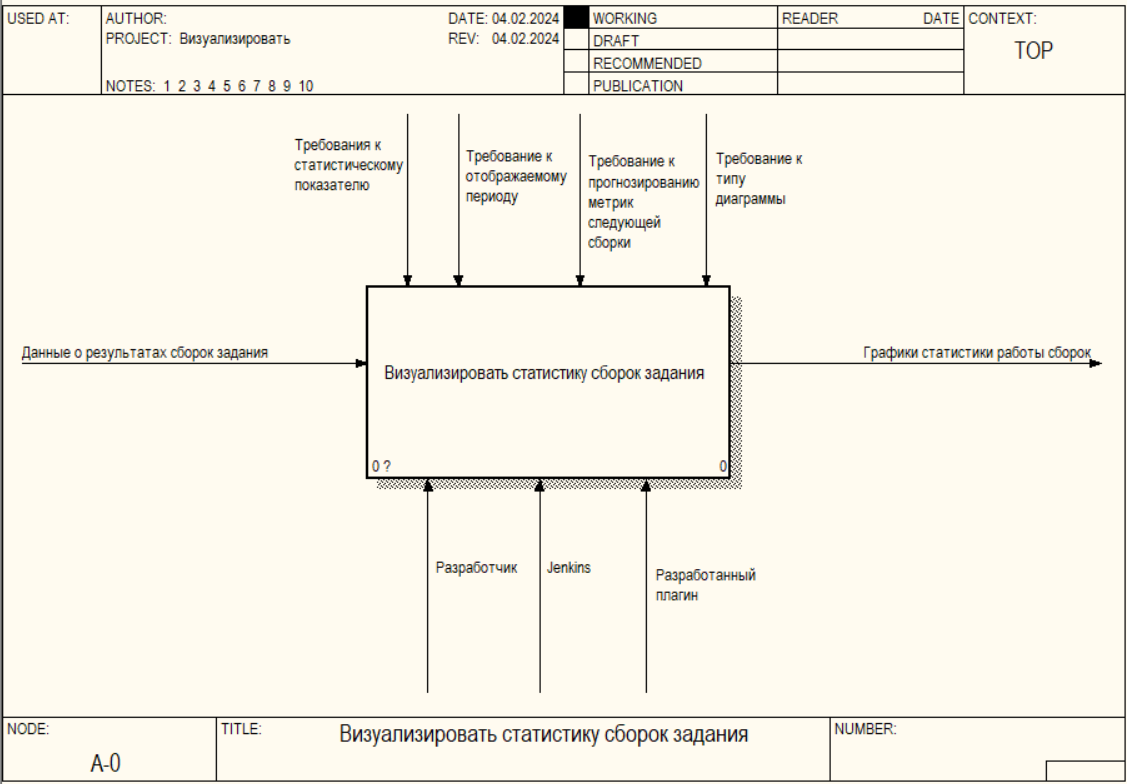
\includegraphics [scale=0.7] {my_folder/images//er1}
	\caption{Процесс визуализации сборок} 
	\label{fig:er1}  
\end{figure}

\begin{figure}[ht!] 
	\center
	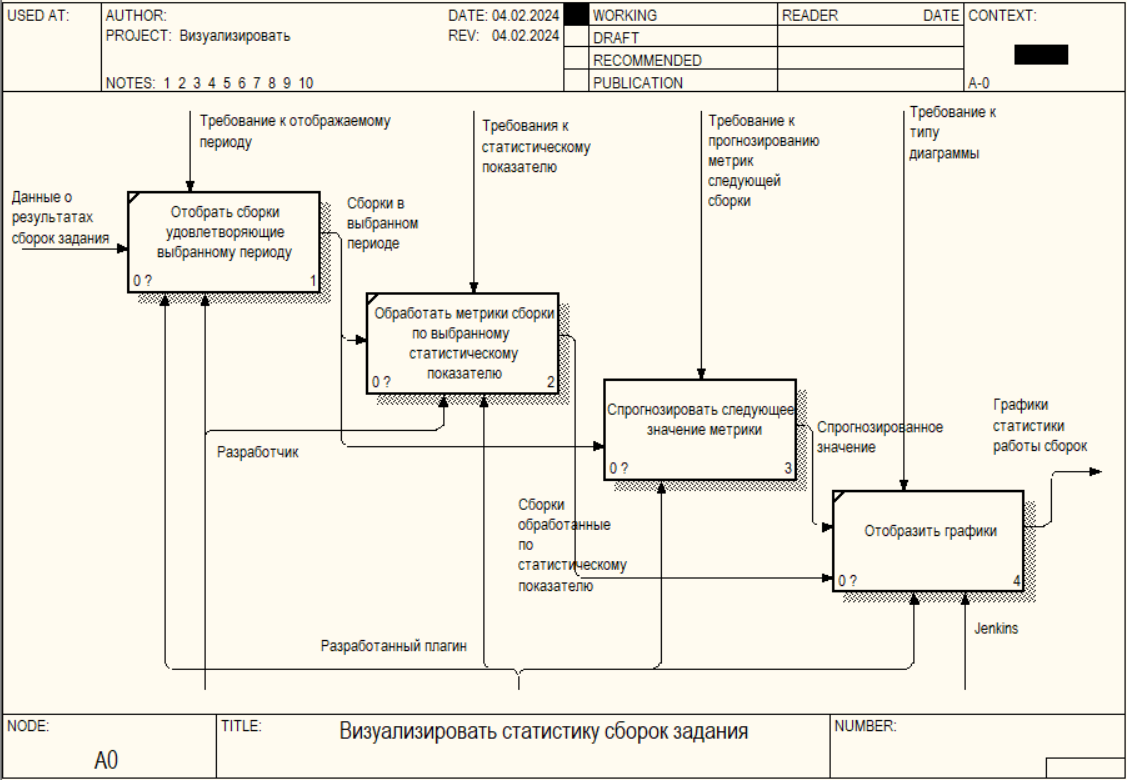
\includegraphics [scale=0.7] {my_folder/images//er2}
	\caption{Детализация процесса визуализации} 
	\label{fig:er2}  
\end{figure}

\begin{figure}[ht!] 
	\center
	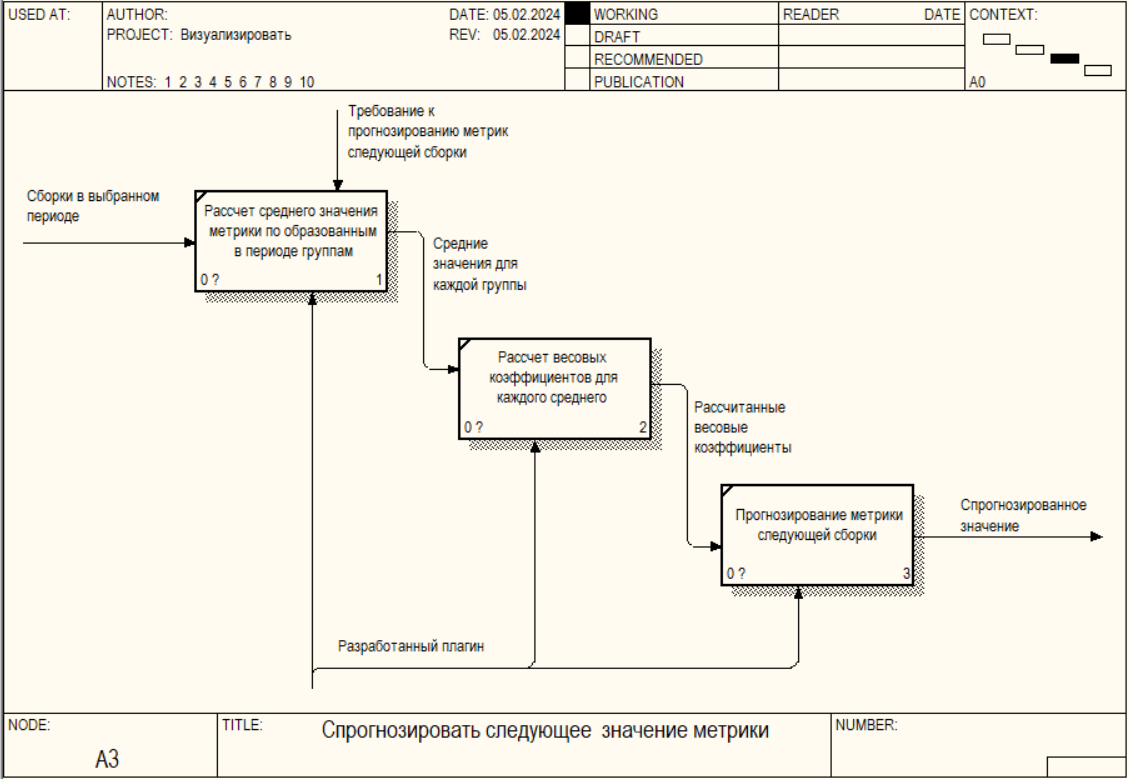
\includegraphics [scale=0.7] {my_folder/images//er3}
	\caption{Процесс прогнозирования метрики} 
	\label{fig:er3}  
\end{figure}

			 	 % Приложение 2


\end{document} % конец документа


%%% Удачной защиты ВКР! - Good luck on the thesis defense!
%%
%%% Поддержать проект
%%
%% Запросы на добавление / изменение просим писать на следующей странице:
%% https://github.com/ParkhomenkoV/SPbPU-student-thesis-template/issues
%%
%% Список пожеланий в файле шаблона <<TO-DO-list.tex>>
%%
%% Благодарности просим указывать в виде 
%%
%% 1. Добавление <<Звезды>> проекту https://github.com/ParkhomenkoV/SPbPU-student-thesis-template/stargazers
%%
%% 2. Добавления <<Сердечка>> и репоста проекта в социальных сетях:
%%		https://vk.com/latex_polytech 
%%		https://www.fb.com/groups/latex.polytech
%%

%%% Support project
%%
%% Requests on adding / modifications is better to be publishen on the following web-page:
%% https://github.com/ParkhomenkoV/SPbPU-student-thesis-template/issues
%%
%% Wishlist is in the template's file called <<TO-DO-list.tex>>
%%
%% Acknowledgements are better to be done in the form of 
%%
%% 1. Adding <<Star>> to the project https://github.com/ParkhomenkoV/SPbPU-student-thesis-template/stargazers
%%
%% 2. Adding <<Likes>> and Project repost in the social networks:
%%		https://vk.com/latex_polytech 
%%		https://www.fb.com/groups/latex.polytech
%% 

% Check list при передаче ВКР:
% - Количество страниц в Задании 2. Если нет, то комментирование последней строки в my_task.tex
% - Зачистка всех вспомогательных файлов (Clear auxilary files) и компиляция ВКР не менее 3х раз